\documentclass[a4paper,11pt,dvipdfmx]{jsarticle}

\usepackage{bm}
\usepackage[dvipdfmx]{graphicx}
\usepackage[dvipdfmx]{color}
\usepackage{ascmac}
\usepackage{siunitx}
\usepackage{otf}
\pagestyle{plain}
\usepackage{float}
\usepackage[dvipdfmx]{hyperref}
\usepackage{pxjahyper}
\usepackage{here}
\usepackage{titlesec}
\usepackage{amsmath,amssymb} %北野加筆
\renewcommand{\bibname}{参考文献} %北野加筆
\titleformat*{\section}{\LARGE\bfseries}
\titleformat*{\subsection}{\normalsize\bfseries}
\usepackage[subrefformat=parens]{subcaption}
\usepackage{url}
\usepackage{comment}
\usepackage{docmute}
\setcounter{page}{0}
\usepackage[table,xcdraw]{xcolor}
\hypersetup{% hyperrefオプションリスト
setpagesize=false,
 bookmarksnumbered=true,%
 bookmarksopen=true,%
 colorlinks=true,%
 linkcolor=blue,
 citecolor=blue,
}
\makeatletter
	\renewcommand{\theequation}{% 式番号の付け方
	\thesection.\arabic{equation}}
	\@addtoreset{equation}{section}

	\renewcommand{\thefigure}{% 図番号の付け方
	\thesection.\arabic{figure}}
	\@addtoreset{figure}{section}

	\renewcommand{\thetable}{% 表番号の付け方
	\thesection.\arabic{table}}
	\@addtoreset{table}{section}
\makeatother


\begin{document}
\documentclass[a4paper,11pt]{jsarticle}
\usepackage{bm}
\usepackage[dvipdfmx]{graphicx}
\usepackage{ascmac}
\usepackage{otf}
\pagestyle{plain}
%\setcounter{page}{}
\usepackage[dvipdfmx]{hyperref}
\usepackage{pxjahyper}

\begin{document}
\begin{center}
{\Large 令和二年度 卒業研究}\\
{\HUGE ポリエチレン標的を用いた\\陽子散乱実験}\\
\vspace*{8cm}
{\LARGE 北野亮輔}\\
{\LARGE 大谷萌}\\
{\LARGE 金\UTF{FA11}奎}\\
{\LARGE 木村将}\\
\vspace*{0.5cm}
{\LARGE 神戸大学理学部物理学科 粒子物理学研究室}\\
\vspace*{2cm}
{\LARGE 2021年 3月19日}
\end{center}
\thispagestyle{empty}

\newpage
\thispagestyle{empty}
 
\newpage
{\LARGE 概要}\\

Ernest Rutherford(1871)は$\alpha$線や$\beta$線の発見、人工的な核変換の成功、など多くの功績を残し、「原子核物理学の父」と呼ばれている。彼の業績の中で最も広く知られているのがRutherfordの散乱実験における原子核の発見であろう。それまで原子の構造については、J.J.Tomsonによるいわゆる「ブドウパンモデル」などが提唱されていたが、広く受け入れられなかった。Rutherfordらは実験の中で$\alpha$線を金原子に照射すると、その一部が大きな偏向角を持って散乱されることを発見した。この結果から、原子の中心に正電荷を持つ小さな核があり、その周囲を電子が回転運動しているという「Rutherfordの原子模型」を提唱した。

本研究では標的にポリエチレンと金を採用し、神戸大学海事科学部にあるタンデム静電加速器を用いて3MeVの陽子を入射した。各散乱角度における微分散乱断面積を求めることによって理論値との比較を行い、原子核の半径やその大きさによるRutherfordの散乱公式の補正や、同種粒子の散乱を見ることを目指した。


\thispagestyle{empty}

\newpage
\thispagestyle{empty}
\setcounter{tocdepth}{3}
\tableofcontents
\thispagestyle{empty}
\thispagestyle{empty}
\end{document}



\documentclass[a4paper,11pt,dvipdfmx]{jsarticle}

\usepackage{bm}
\usepackage[dvipdfmx]{graphicx}
\usepackage[dvipdfmx]{color}
\usepackage{ascmac}
\usepackage{siunitx}
\usepackage{otf}
\pagestyle{plain}
\usepackage{float}
\usepackage[dvipdfmx]{hyperref}
\usepackage{pxjahyper}
\usepackage{here}
\usepackage{titlesec}
\titleformat*{\section}{\LARGE\bfseries}
\titleformat*{\subsection}{\normalsize\bfseries}
\usepackage{url}
\usepackage[table,xcdraw]{xcolor}
\hypersetup{% hyperrefオプションリスト
setpagesize=false,
 bookmarksnumbered=true,%
 bookmarksopen=true,%
 colorlinks=true,%
 linkcolor=blue,
 citecolor=blue,
}

\begin{document}
\newpage
\section{\LARGE{導入と理論(担当:北野)}}

\subsection{実験の目的と概要}
我々は、神戸大学深江キャンパスにあるタンデム加速器を用いてポリエチレン標的を用いた陽子の散乱実験を行った。本実験の目的は、2つの検出器を用いて陽子-陽子散乱(p-p散乱)の同時計測を行うこと、またポリエチレンに含まれる炭素原子核によって散乱される陽子の微分散乱断面積を測定し、炭素の原子核半径を求めることである。

本論文では本実験の理論、実験装置、データ収集と解析、議論と考察について述べる。

\end{document}
\documentclass[a4paper,11pt,dvipdfmx]{jsarticle}

\usepackage{bm}
\usepackage[dvipdfmx]{graphicx}
\usepackage[dvipdfmx]{color}
\usepackage{ascmac}
\usepackage{amsmath}
\usepackage{amssymb}
\usepackage{siunitx}
\usepackage{otf}
\usepackage[dvipdfmx]{graphicx}
\pagestyle{plain}
\usepackage{float}
\usepackage[dvipdfmx]{hyperref}
\usepackage{pxjahyper}
\usepackage{here}
\usepackage{titlesec}
\titleformat*{\section}{\LARGE\bfseries}
\titleformat*{\subsection}{\normalsize\bfseries}
\usepackage{url}
\usepackage[table,xcdraw]{xcolor}
\hypersetup{% hyperrefオプションリスト
setpagesize=false,
 bookmarksnumbered=true,%
 bookmarksopen=true,%
 colorlinks=true,%
 linkcolor=blue,
 citecolor=blue,
}

\begin{document}
\setcounter{page}{1}
\renewcommand\thefootnote{\arabic{footnote})}
\subsection{微分散乱断面積の理論}
本節では今回の散乱実験で重要な物理量となる微分散乱断面積について考える。
ここでは微分散乱断面積を重心系における散乱角$\theta$で定義する。
\subsubsection{異なる2粒子系におけるCoulomb散乱\cite{2017}\cite{ion}}
加速された陽子がターゲットに入射して散乱する主な原因としてCoulomb力による散乱(Rutherford散乱)が考えられる。本節では異なる2粒子系についてRutherford散乱がどのように表されるかを量子論的に考える。

今、中心力が働く場に対する入射粒子の相対運動を考え、入射粒子を平面波、散乱粒子を球状波で表し、図\ref{fig:qmscattering}のように座標を取る。また、異なる2粒子の原子番号を$Z_{1}$,$Z_{2}$とする。
\begin{figure}[hbtp]
\centering
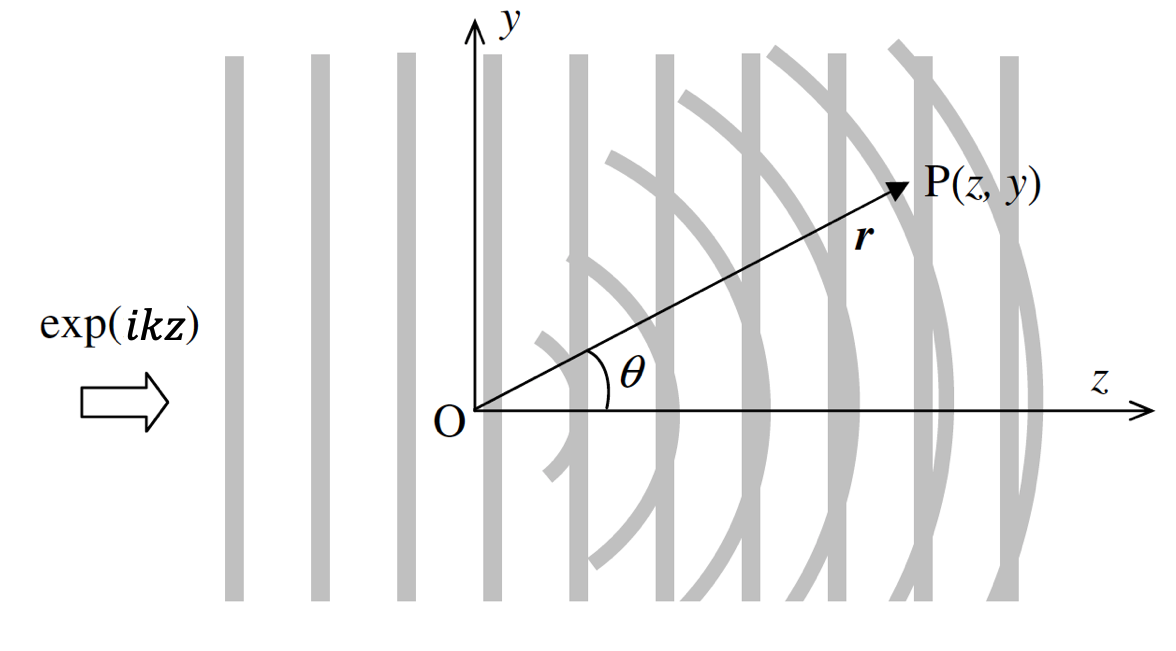
\includegraphics[width=10cm]{picture/cstheory/qmscattering.png}
\caption{散乱角$\theta$、入射方向$z$の散乱の様子(\cite{ion}より引用し、一部改変)}
\label{fig:qmscattering}
\end{figure}

クーロン相互作用している2粒子系のSchrödinger方程式はCoulombポテンシャル
\begin{equation*}
    V(r)=\frac{Z_{1}Z_{2}e^{2}}{4\pi\varepsilon_{0}r} 
\end{equation*}
を用いて
\begin{equation}
\left(-\frac{\hbar^{2}}{2m}\Delta + \frac{Z_{1}Z_{2}e^{2}}{4\pi\varepsilon_{0}r}\right)\Psi =E\Psi
\label{eq:sch}
\end{equation}
のように書くことができる。ここで、
\begin{equation}
E=\frac{\hbar^{2}k^{2}}{2m}=\frac{1}{2}mv^{2}
\end{equation}
は重心系における運動エネルギーである。極座標から放物線座標への変換式
\begin{gather*}     
      \xi\,=\, r - z \,=\, r\left(1 - \cos\theta\right), \\  
      \eta\,=\, r + z \,=\, r\left(1 + \cos\theta\right), \\
      \psi\,=\,\psi. 
\end{gather*}
を用いて式\eqref{eq:sch}を変換すると、
\begin{equation}
-\frac{\hbar^{2}}{2m}\frac{4}{\xi+\eta}\left[\frac{\partial}{\partial\xi}\left(\xi\frac{\partial\Psi}{\partial\xi}\right)+ \frac{\partial}{\partial\eta}\left(\eta\frac{\partial\Psi}{\partial\eta}\right)\right]+ \frac{Z_{1}Z_{2}e^{2}}{2\pi\varepsilon_{0}\left(\xi+\eta\right)}\Psi =E\Psi
\label{eq:sch2}
\end{equation}
となる。

ここで$\Psi$を
\begin{equation}
    \Psi = \exp(ikz)\chi\left(r,\theta\right)=  \exp\left[-ik\left(\xi-\eta\right)/2\right]\chi\left(\xi,\eta\right)
    \label{eq:Psi}
\end{equation}
とする。

今、$\Psi$は遠方では外向きの球状波に漸近すべきなので、式\eqref{eq:Psi}より、$\chi$は遠方で \\*\:$\exp[ik(r-z)] \,=\,\exp(ik\xi)$\,という項に比例するはずである。ところで、式\eqref{eq:sch2}より$\Psi$は$\xi$と$\eta$を交換しても不変なので、$\chi$が変数$\eta$を含むとすれば、$\chi$は遠方では $\exp(ik\eta) \,=\,\exp[(ik(r+z)]$\, \\
という項に比例することになる。しかし、これは逆向きの入射波に相当するものであり、 \\
不適切である。よって、$\chi$は$\eta$を含まない。

式\eqref{eq:Psi}を式\eqref{eq:sch2}に代入し、$\chi$が$\xi$のみの関数であることを考慮して、
\begin{equation}
    \xi\frac{d^{2}\chi}{d\xi^{2}} + \left(1 - ik\xi\right)\frac{d\chi}{d\xi} -\frac{\kappa k}{2}\chi = 0
    \label{eq:tyokika}
\end{equation}
を得る。ここで
\begin{gather*}
\kappa = \frac{Z_{1}Z_{2}e^{2}}{2\pi\varepsilon_{0}\hbar v}
\end{gather*}
であり、BohrのCoulomb散乱パラメータと呼ばれる無次元数である。\footnote{$\dfrac{\kappa}{2}$をBohrのCoulomb散乱パラメータと呼ぶ流儀もある。}

この解を求めるために合流型超幾何関数を考える。一般に$A$,$B$を定数として
\begin{equation}
        X\frac{d^{2}F}{dX^{2}} + \left(B - X\right)\frac{dF}{dX} -AF = 0
        \label{eq:tyo}
\end{equation}
の解$F$を合流型超幾何関数と呼ぶ。$X=0$で正則なものの解は、
\begin{align} 
     F(A,B,X) &= \sum_{j=0}^{\infty}\frac{\Gamma\left(A+j\right)\Gamma\left(B\right)X^{j}}{\Gamma\left(A\right)\Gamma\left(B+j\right)\Gamma\left(1+j\right)} \notag\\
    &= 1+ \frac{A}{B1!}X+\frac{A\left(A+1\right)}{B\left(B+1\right)2!}X^{2}+\frac{A\left(A+1\right)\left(A+2\right)}{B\left(B+1\right)\left(B+2\right)3!}X^{3}+\cdots 
    \label{eq:tyokika2}
  \end{align}

と表される。$\Gamma$はRe$(z)>0$の時
\begin{equation*}
    \Gamma(z)= \int_{0}^{\infty}e^{-t}t^{z-1}dt
\end{equation*}
で定義される$\Gamma$関数である。

式\eqref{eq:tyokika}を
\begin{equation*}
   ik\xi\frac{d^{2}\chi}{d\left(ik\xi\right)^{2}} + \left(1 - ik\xi\right)\frac{d\chi}{d\left(ik\xi\right)} -\frac{-i\kappa}{2}\chi = 0 
\end{equation*}
と変形し、\eqref{eq:tyo}と比較すると、解$\chi$は
\begin{displaymath}
\chi=F\left(\frac{-i\kappa}{2},\,1,\,ik\xi\right)
\end{displaymath}
となる。規格化した式\eqref{eq:sch}の解は、
\begin{align}
     \Psi \,&=\, \exp\left(-\frac{\pi\kappa}{4}+ikz\right)\Gamma\left(1+\frac{i\kappa}{2}\right)F\left(\frac{-i\kappa}{2},\,1,\,ik\xi\right) \notag\\
     &= \,\exp\left(-\frac{\pi\kappa}{4}+ikr\cos\theta\right)\Gamma\left(1+\frac{i\kappa}{2}\right)F\left(\frac{-i\kappa}{2},\,1,\,2ikr\sin^2\frac{\theta}{2}\right) \notag\\
     &= \,\left(1 - \frac{i\kappa^{2}}{8kr\sin^2\frac{\theta}{2}}\right)\exp\left(i[kr\cos\theta+\frac{\kappa}{2}\ln(2kr\sin^2\frac{\theta}{2})]\right) \notag\\
     &+ \,\frac{\kappa}{4kr\sin^2\frac{\theta}{2}}\exp\left(i[kr-\frac{\kappa}{2}\ln(2kr\sin^2\frac{\theta}{2})+\pi+2\eta_{0}]\right)\label{eq:kikakukai}
\end{align}
と表される。ただし、2行目から3行目の変形の際、$kr\gg1$,すなわち入射粒子のde  Broglie波長$(2\pi/k)$に比べて$r$が十分大きいとした。また、$\exp(2i\eta_{0})=\Gamma(1+i\kappa/2)/\Gamma(1-i\kappa/2)$である。

式\eqref{eq:kikakukai}の第一項は透過波、第二項は散乱波とみなせる。$kr\rightarrow \infty$とすると、\\*
$\Psi = \exp(ikr\cos\theta)  =\exp(ikz)$、つまり第一項の入射(透過)波のみとなって、散乱波は無視されてしまうことに注意する。遠方では、$kr\gg\ln{kr}$なので式\eqref{eq:kikakukai}の漸近形は
\begin{equation}
 \Psi \sim \exp(ikz)+f(\theta)\,\frac{\exp(ikr)}{r} 
 \label{eq:zenkinn}
\end{equation}
のようになる。このとき、$\kappa$と$k$を戻して係数比較すれば、
\begin{equation}
    f(\theta)=\frac{Z_{1}Z_{2}e^2}{8\pi\varepsilon_{0}mv^2}\exp\left(i[-\frac{\kappa}{2}\ln(2kr\sin^2\frac{\theta}{2})+\pi+2\eta_{0}]\right)\frac{1}{\sin^2\frac{\theta}{2}}
    \label{eq:sanransinpuku}
\end{equation}
となり、この式\eqref{eq:sanransinpuku}はCoulomb散乱の散乱振幅と呼ばれる。
微分散乱断面積は散乱振幅の絶対値の2乗で表されるので、
\begin{align}
    \frac{d\sigma}{d\Omega} = |f(\theta)|^{2}=\left(\frac{Z_{1}Z_{2}e^2}{8\pi\varepsilon_{0}mv^2}\right)^{2}\frac{1}{\sin^4\frac{\theta}{2}} \notag\\
    = \left(\frac{Z_{1}Z_{2}e^2}{16\pi\varepsilon_{0}E}\right)^{2}\frac{1}{\sin^4\frac{\theta}{2}}\label{eq:Rutherford}
\end{align}
式\eqref{eq:Rutherford}をRutherfordの散乱公式という。

今回の実験では陽子を入射させるので、Rutherfordの散乱公式は以下のように書ける。
\begin{equation}
    \frac{d\sigma}{d\Omega}=\left(\frac{Ze^2}{16\pi\varepsilon_{0}E}\right)^{2}\frac{1}{\sin^4\frac{\theta}{2}}\label{eq:Ruther}
\end{equation}
$Z$はターゲットの原子番号、$E$は入射粒子のエネルギー、$\theta$は重心系における散乱角である。
\eqref{eq:Ruther}を今回の実験で用いる標的ごとにグラフに表すと図\ref{fig:cross}のようになる。
($E=$\;3\;MeV) 
\\
\\
\begin{figure}[htbp]
\centering
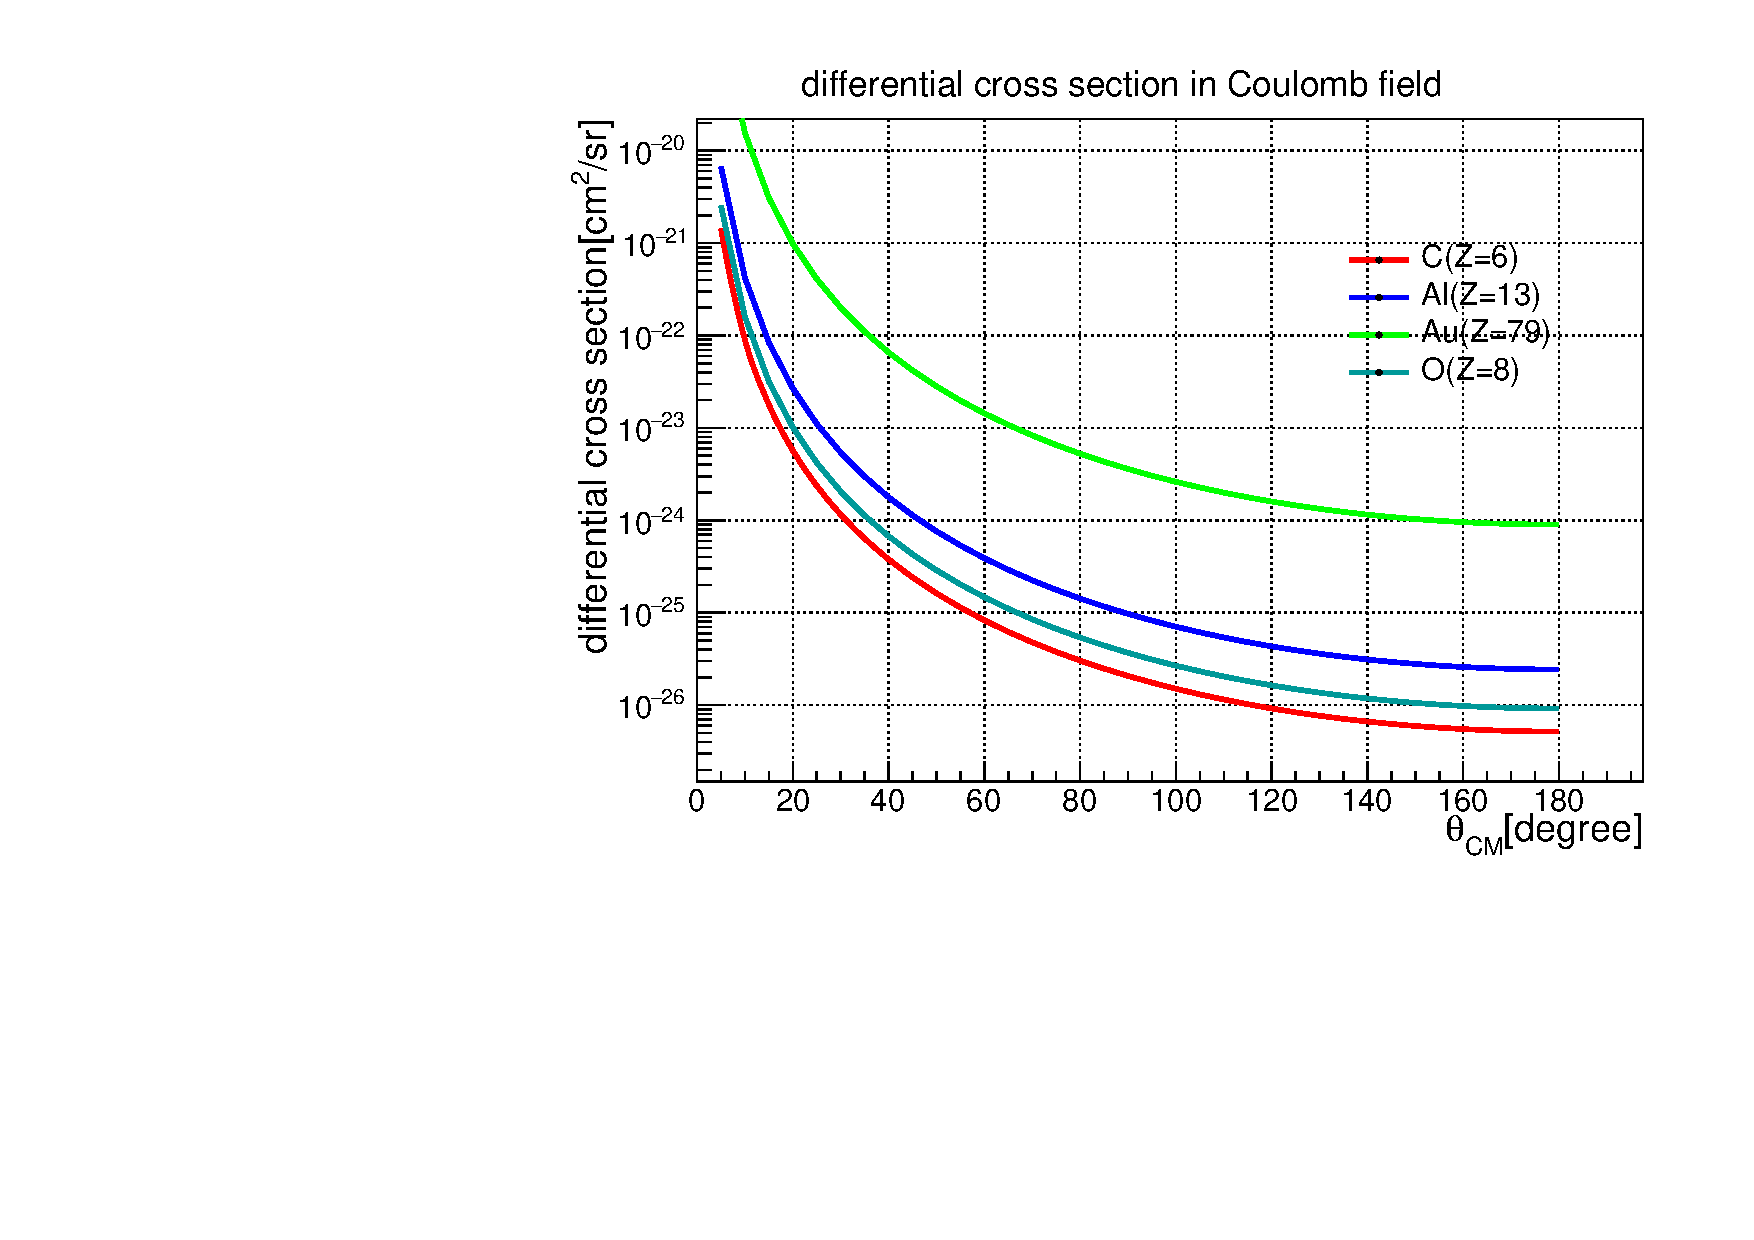
\includegraphics[width=9cm]{picture/cstheory/newcr.pdf}
\caption{クーロン力による微分散乱断面積}
\label{fig:cross}
\end{figure}

\newpage
\subsubsection{同種2粒子系におけるCoulomb散乱\cite{2017}}
以下では、便宜上2つの粒子をそれぞれ粒子1、粒子2と呼称する。

同種粒子の場合、2粒子が異なる場合と比べて以下の2点を修正する必要がある。
\begin{enumerate}
    \item 検出器は粒子1と粒子2を実験的に区別することができないため、断面積$\sigma$を定義し直す必要がある。
    \item 波動関数を定義し直す必要がある。
\end{enumerate}

1つ目については量子力学固有のものではない。p-p散乱では図\ref{fig:ppcm}のような黒と青の2つの経路が考えられる。
今、粒子1の断面積を$\sigma^{(1)}$、粒子2の断面積を$\sigma^{(2)}$とすると、検出器における断面積はそれらの和で書けるため、
\begin{equation*}
    \sigma=\sigma^{(1)}+\sigma^{(2)}
\end{equation*}
と定義できる。ここで$\sigma^{(1)}$は散乱振幅$f(\theta)$を使って、
\begin{equation*}
    \sigma^{(1)}=|f(\theta)|^{2}
\end{equation*}
と表されるとすると、粒子2のほうは重心系で考えているため、
\begin{equation*}
    \sigma^{(2)}=|f(\pi-\theta)|^{2}
\end{equation*}
と表される。
\begin{figure}[htbp]
\centering
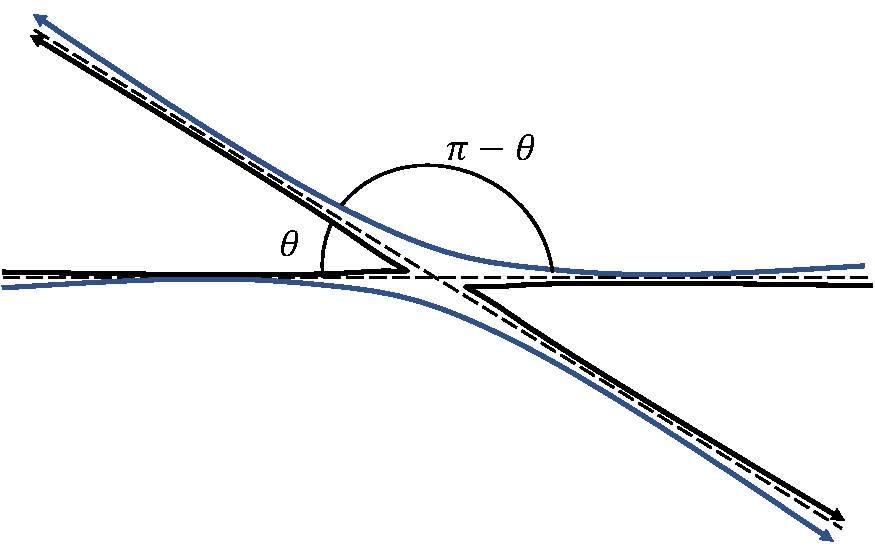
\includegraphics[width=7cm]{picture/cstheory/p-pCM.pdf}
\caption{重心系におけるp-p散乱}
\label{fig:ppcm}
\end{figure}

2つ目については量子力学固有のものである。以下の議論で「対称化する」とは、ボゾンなら完全対称に、フェルミオンなら反対称にすることである。修正前の波動関数の漸近形は\eqref{eq:zenkinn}の形で与えられたが、第一項を$\Psi_{i}$、第二項を$\Psi_{d}$とすると、対称化した波動関数$\Psi'$は
\begin{equation*}
    \Psi'=\Psi_{i}\pm\Psi'_{i}+\Psi_{d}\pm\Psi'_{d}
\end{equation*}
と表せる。$\pm$は$+$がボゾン、$-$がフェルミオンである。ただし、
\begin{align*}
    \Psi'_{i}(\theta)\sim \Psi_{i}(\pi-\theta) \\
    \Psi'_{d}(\theta)\sim \Psi_{d}(\pi-\theta)
\end{align*}
である。よって、$\Psi'$は以下のように表すことができる。
\begin{equation}
    \Psi' \sim \exp(ikz) \pm \exp(-ikz)+f'(\theta)\frac{\exp(ikr)}{r} 
\end{equation}
ただし、
\begin{equation*}
    f'(\theta)=f(\theta)+f(\pi-\theta)
\end{equation*}
であり、対称化振幅と呼ばれる。これで2つの修正ができたことになる。よって、微分散乱断面積は
\begin{equation*}
    \frac{d\sigma}{d\Omega}=|f'(\theta)|^{2}=|f(\theta)+f(\pi-\theta)|^{2}
\end{equation*}
となる。

しかし、今回考える陽子はスピン$\tfrac{1}{2}$を持つのでそのことも考慮しなくてはいけない。そのため、まず一般的にスピンが$s$の同種2粒子の散乱を考える。2粒子の合成スピンの状態の波は全部で\((2s+1)^2\)個あり、1重項状態が1個、3重項状態が3個、$\cdots$、$(4s+1)$重項状態が$(4s+1)$個となっている。$(4t+1)$重項状態に対応する散乱振幅を$f_{4t+1}(\theta)$で表す。
(ただし、$t=0,\tfrac{1}{2},1,\tfrac{3}{2},\cdots,s$) \\*
$t$が整数の時、$(4t+1)$重項に対応する微分散乱断面積は
\begin{equation*}
    \frac{d\sigma}{d\Omega_{4t+1}}=|f_{4t+1}(\theta)+f_{4t+1}(\pi-\theta)|^2
\end{equation*}
であり、$t$が半整数の時、$(4t+1)$重項に対応する微分散乱断面積は
\begin{equation*}
    \frac{d\sigma}{d\Omega_{4t+1}}=|f_{4t+1}(\theta)-f_{4t+1}(\pi-\theta)|^2
\end{equation*}
と表される。

偏りのない粒子同士の衝突において、入射粒子と標的粒子のスピンの方向は偶然に決められるので、微分散乱断面積の計算は重みをつけて考える。だから、
\begin{align}
    \frac{d\sigma}{d\Omega} &= \frac{1}{(2s+1)^{2}}[|f_{1}(\theta)+f_{1}(\pi-\theta)|^{2}+3\,|f_{3}(\theta)-f_{3}(\pi-\theta)|^{2} \notag\\
    &+ \cdots +(4s+1)\,|f_{4s+1}(\theta)+(-1)^{2s}f_{4s+1}(\pi-\theta)|^{2}]\label{eq:spin}
\end{align}
今、クーロン散乱のみを考えているため、散乱振幅にスピンは無関係で、
\begin{equation}
    f_{4t+1}(\theta)=f(\theta) \ \ (t=0,\frac{1}{2},1,\frac{3}{2},\cdots,s)\label{eq:mukankei}
\end{equation}
とできる。

よって、式\eqref{eq:spin}と式\eqref{eq:mukankei}より、
\begin{align}
     \frac{d\sigma}{d\Omega} &= \frac{1}{(2s+1)^{2}}[|f_{1}(\theta)+f_{1}(\pi-\theta)|^{2}+3\,|f_{3}(\theta)-f_{3}(\pi-\theta)|^{2} \notag\\
    &+ \cdots +(4s+1)\,|f_{4s+1}(\theta)+(-1)^{2s}f_{4s+1}(\pi-\theta)|^{2}] \notag\\
 &= |f(\theta)|^2+|f(\pi-\theta)|^2\notag\\
     &+\frac{1}{(2s+1)^{2}}[1-3+5-\cdots+(-1)^{2s}(4s+1)][f(\theta)f^*(\pi-\theta)+f^*(\theta)f(\pi-\theta)] \notag\\
 &= |f(\theta)|^2+|f(\pi-\theta)|^2\notag\\
   &+\frac{1}{(2s+1)^{2}}\,2\,(-1)^{2s}(2s+1)[f(\theta)f^*(\pi-\theta)+f^*(\theta)f(\pi-\theta)] \notag\\
    &= |f(\theta)|^2+|f(\pi-\theta)|^2 +(-1)^{2s}\frac{2}{(2s+1)}[f(\theta)f^*(\pi-\theta)+f^*(\theta)f(\pi-\theta)] 
\end{align}
これに散乱振幅$f(\theta)$の式\eqref{eq:sanransinpuku}を代入すると、
\begin{equation}
   \frac{d\sigma}{d\Omega} = \left(\frac{Z_{1}Z_{2}e^2}{16\pi\varepsilon_{0}E}\right)^{2}\left[\frac{1}{\sin^4\frac{\theta}{2}}+\frac{1}{\cos^4\frac{\theta}{2}}+(-1)^{2s}\frac{2}{2s+1}\frac{\cos[\frac{Z_{1}Z_{2}e^2}{4\pi\varepsilon_{0}\hbar v}\ln(\tan^2\frac{\theta}{2})]}{\sin^2\frac{\theta}{2}\cos^2\frac{\theta}{2}}\right]
   \label{eq:dousyucs}
\end{equation}
今回はp-p散乱(陽子-陽子散乱)なので、$Z_{1}=Z_{2}=1,s=\frac{1}{2}$を\eqref{eq:dousyucs}に代入すると、
\begin{equation}
   \frac{d\sigma}{d\Omega} = \left(\frac{e^2}{16\pi\varepsilon_{0}E}\right)^{2}\left[\frac{1}{\sin^4\frac{\theta}{2}}+\frac{1}{\cos^4\frac{\theta}{2}}-\frac{\cos[\frac{e^2}{4\pi\varepsilon_{0}\hbar v}\ln(\tan^2\frac{\theta}{2})]}{\sin^2\frac{\theta}{2}\cos^2\frac{\theta}{2}}\right]
   \label{eq:Mott}
\end{equation}
となる。式\eqref{eq:Mott}をMottの散乱公式という。

本実験では$E=$\;3\;MeVなので、この場合の式\eqref{eq:Mott}のグラフは図\ref{fig:Mott}のようになる。図\ref{fig:Mott}より、微分散乱断面積は散乱角$90^{\circ}$を境に対称的な形をとることがわかる。
\begin{figure}[htbp]
\centering
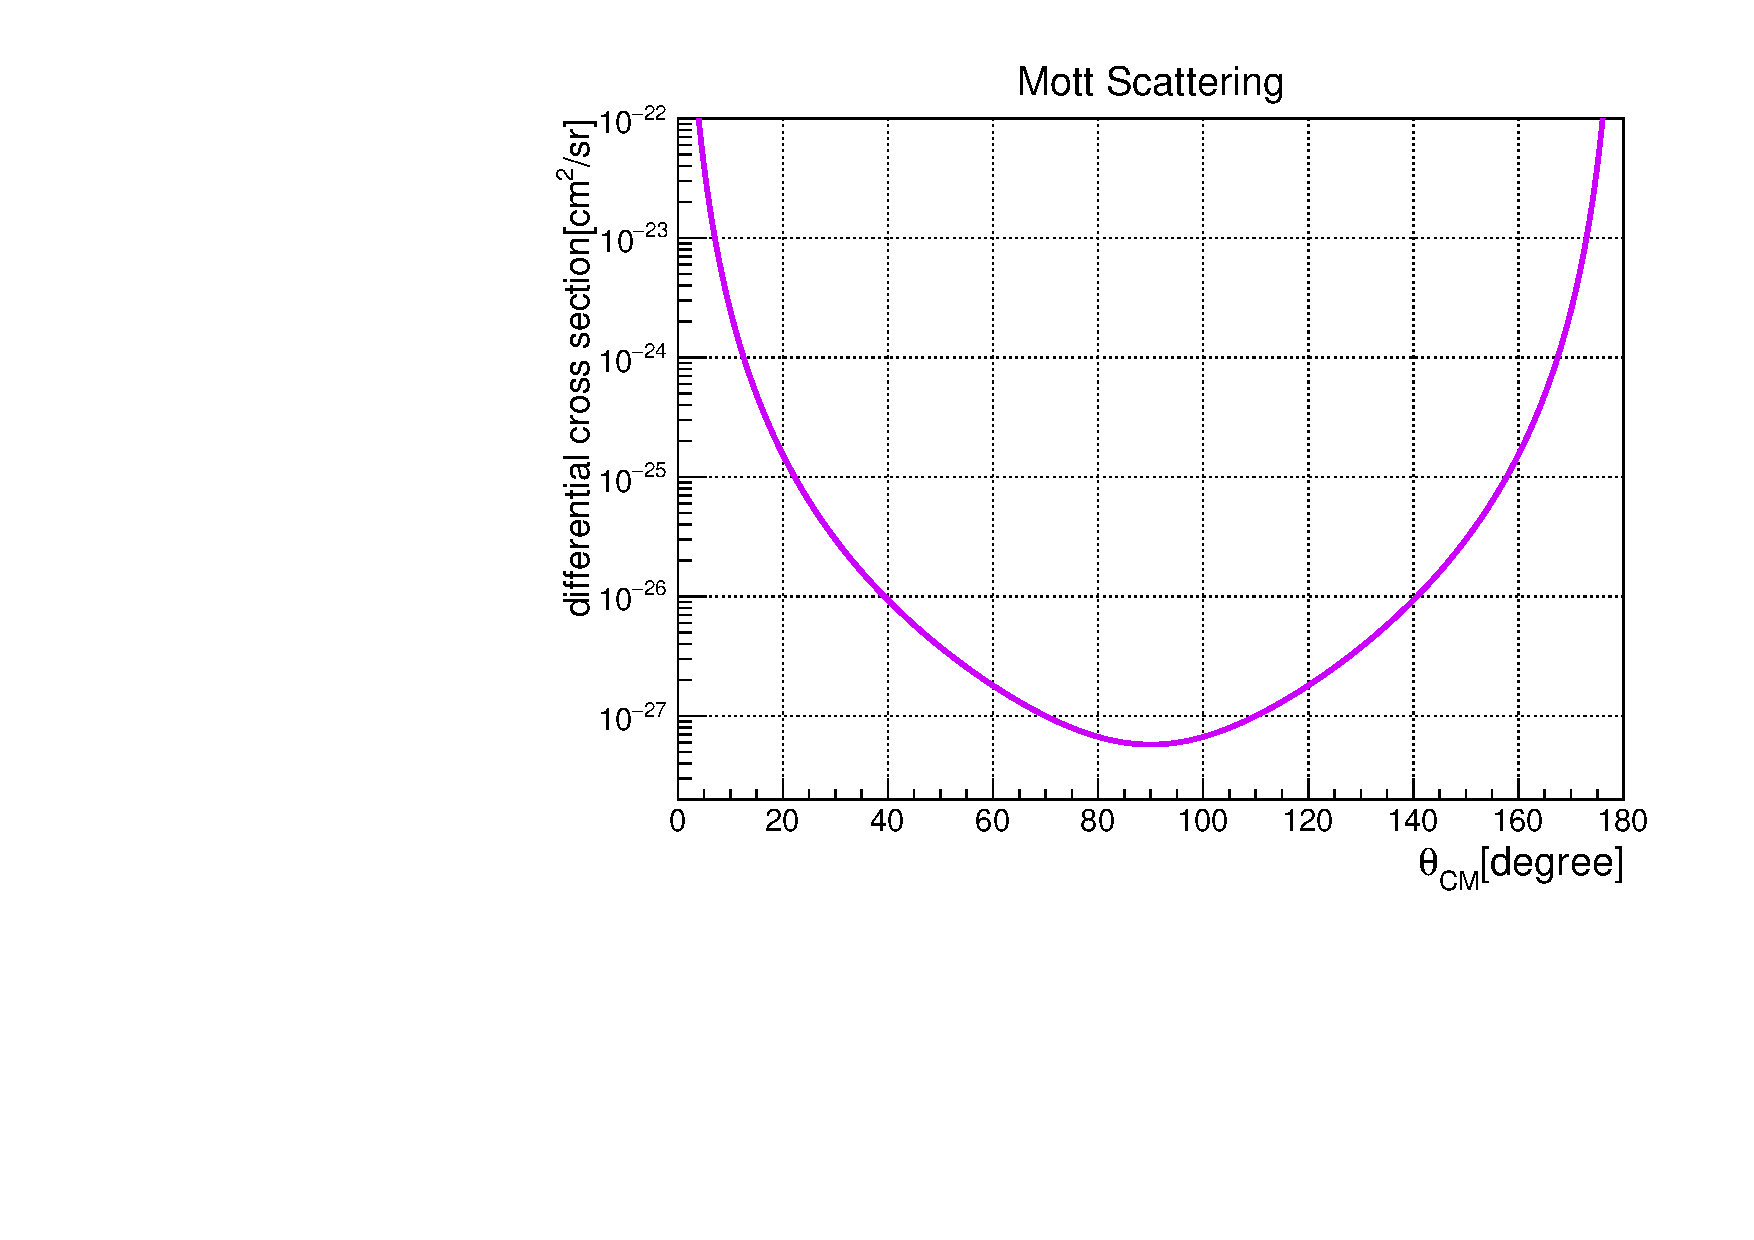
\includegraphics[width=9cm]{picture/cstheory/Mott_revise.pdf}
\caption{Mott散乱による微分散乱断面積}
\label{fig:Mott}
\end{figure}

\newpage
\subsubsection{核力による散乱}\label{NF}
加速された陽子が標的となる試料に入射したときに散乱される要因として、核力による散乱も考えられる。ここでは古典的に、陽子と標的原子核の衝突を剛体球による散乱と近似し、剛体球による微分断面積を考える。

\begin{figure}[htbp]
\centering
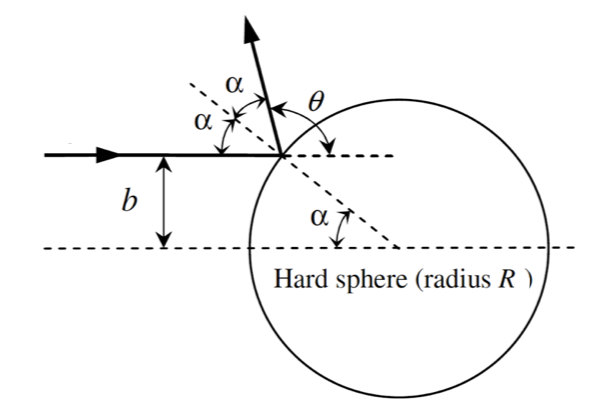
\includegraphics[width=7cm]{picture/cstheory/NF.png}
\caption{剛体球による散乱の様子(\cite{ion}より引用し、一部改変)}
\label{fig:NF}
\end{figure}

図\ref{fig:NF}のような状況を考える。この場合の微分散乱断面積は、全立体角$4\pi$に対して陽子から見た球のシルエットの面積の比をとればよく、その面積は$\pi R^{2}$なので、 \\
求める微分散乱断面積は、
\begin{equation}
    \frac{d\sigma}{d\Omega}=\frac{R^{2}}{4}
    \label{eq:nfcr1}
\end{equation}
となる。

陽子半径$r$を考慮する場合は、\eqref{eq:nfcr1}右辺の$R$を$R+r$に書き換えればよく\cite{ion}、この場合の剛体球による微分散乱断面積は、
\begin{equation}
    \frac{d\sigma}{d\Omega}=\frac{(R+r)^{2}}{4}
    \label{eq:nfcr2}
\end{equation}
と表される。

本研究では、核力による散乱を式\eqref{eq:nfcr2}で表される剛体球による散乱として解析を行う。



\end{document}
\documentclass[a4paper,11pt,dvipdfmx]{jsarticle}

\usepackage{bm}
\usepackage[dvipdfmx]{graphicx}
\usepackage[dvipdfmx]{color}
\usepackage{ascmac}
\usepackage{amsmath}
\usepackage{amssymb}
\usepackage{siunitx}
\usepackage{otf}
\usepackage[dvipdfmx]{graphicx}
\pagestyle{plain}
\usepackage{float}
\usepackage[dvipdfmx]{hyperref}
\usepackage{pxjahyper}
\usepackage{here}
\usepackage{titlesec}
\titleformat*{\section}{\LARGE\bfseries}
\titleformat*{\subsection}{\normalsize\bfseries}
\usepackage{url}
\usepackage[table,xcdraw]{xcolor}
\hypersetup{% hyperrefオプションリスト
setpagesize=false,
 bookmarksnumbered=true,%
 bookmarksopen=true,%
 colorlinks=true,%
 linkcolor=blue,
 citecolor=blue,
}

\begin{document}
\renewcommand\thefootnote{\arabic{footnote})}
\newpage
\subsection{原子核半径推定の理論}
前節では本実験において重要な物理量である微分散乱断面積について議論したが、本節ではそれらの議論を元に、本研究の目的である、炭素原子核半径の推定を行うのに必要な理論について論ずることにする。
\subsubsection{最近接距離と原子核半径}
3\;MeVに加速された陽子が標的原子核の中心までどれだけ近づけるのか考える。
式\eqref{eq:saikinsetu}に標的の原子番号$Z$、入射陽子のエネルギー$E=$\;3\;MeV\;$=4.8\times10^{-13}\;$J\,を代入することで最近接距離$r_{min}$を求められる。
\begin{equation}
    r_{min}=\frac{Ze^{2}}{4\pi\varepsilon_{0}E}
    \label{eq:saikinsetu}
\end{equation}

次にターゲットの原子核半径を求める。原子核半径$R$は質量数$A$の1/3乗に比例することが分かっており、以下の式\eqref{eq:radius}で表される。\footnote{本来は近似式であるが、本研究では等式として扱う。}ただし、水素の原子核半径は陽子半径と等しいとみなせるので、式\eqref{eq:radius}には従わない。
\begin{equation}
    R=1.3\times A^{\frac{1}{3}}
    \label{eq:radius}
\end{equation}

表\ref{table:gensi}に各標的ごとに計算された最近接距離と原子核半径を示す。

\begin{table}[htbp]
 \centering
  \begin{tabular}{clll}
   \hline 
   \  & \,Au & \;\,C & \;\,H \\
   \hline \hline
   最近接距離(fm) & 38.7 & 2.94 & 0.49 \\
   原子核半径(fm) & 7.56 & 2.97 & 0.88 \\
   \hline    
  \end{tabular}
  \caption{最近接距離と原子核半径}
   \label{table:gensi}
\end{table}

表\ref{table:gensi}から、炭素原子核と水素原子核(陽子)についてはCoulomb力による散乱だけでなく、核力による散乱を考慮する必要があると分かる。

\subsubsection{炭素の原子核半径}
以上の議論から、炭素原子核についてCoulomb力による散乱と核力による散乱の場合の微分散乱断面積を比較したものが図\ref{fig:hikaku}になる。

図\ref{fig:hikaku}において、青色の線は核力、赤色の線はCoulomb力、水色の線はCoulomb力と核力を足し合わせたものである。

図\ref{fig:hikaku}から、散乱角$80^{\circ}$付近から核力による影響がCoulomb力による影響より大きくなり、より大角度では核力による影響が支配的になると言える。
よって、大角度での微分散乱断面積の測定値から炭素の原子核半径を推定することができる。
\begin{figure}[htbp]
\centering
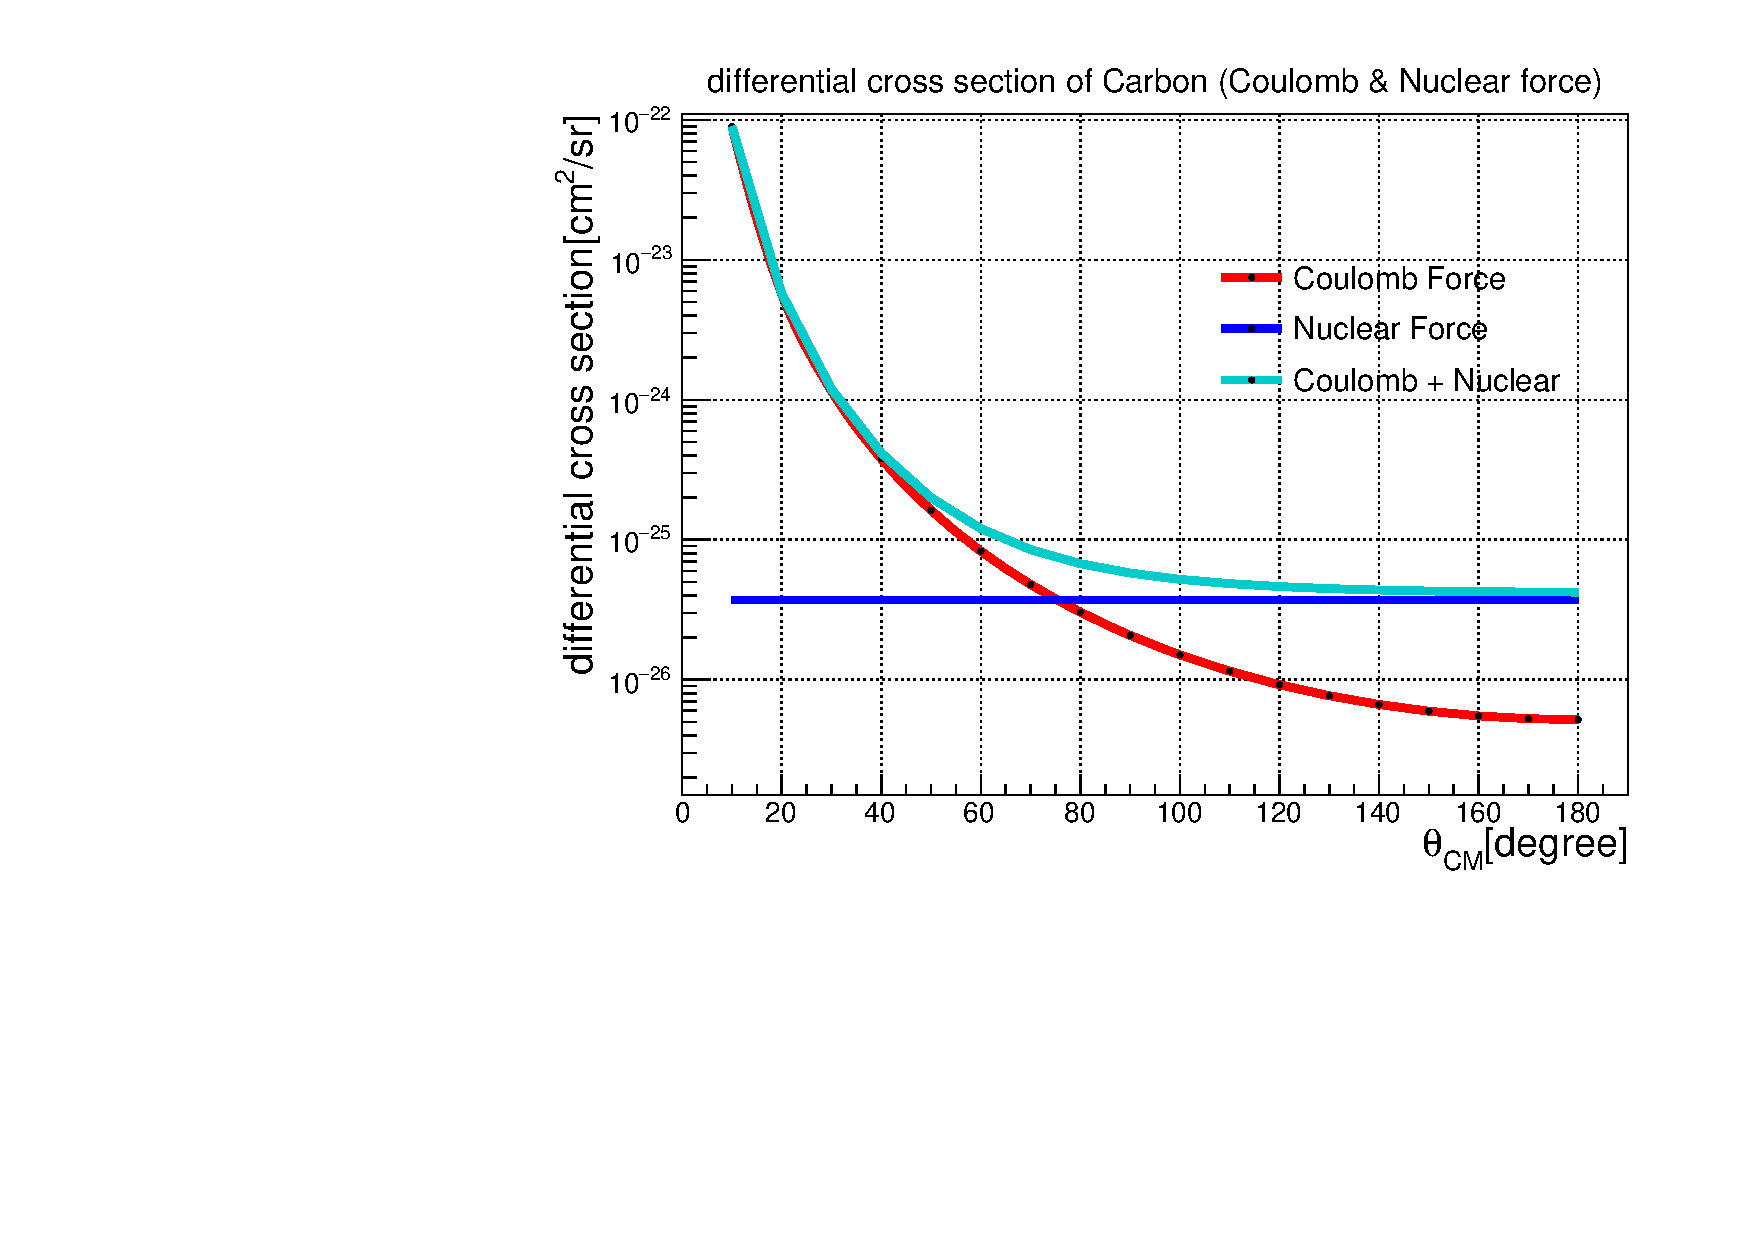
\includegraphics[width=9cm]{picture/radiustheory/kakutei.pdf}
\caption{炭素の微分散乱断面積}
\label{fig:hikaku}
\end{figure}

\end{document}
\documentclass[a4paper,11pt,dvipdfmx]{jsarticle}

\usepackage{bm}
\usepackage[dvipdfmx]{graphicx}
\usepackage[dvipdfmx]{color}
\usepackage{ascmac}
\usepackage{amsmath}
\usepackage{amssymb}
\usepackage{siunitx}
\usepackage{otf}
\usepackage[dvipdfmx]{graphicx}
\pagestyle{plain}
\usepackage{float}
\usepackage[dvipdfmx]{hyperref}
\usepackage{pxjahyper}
\usepackage{here}
\usepackage{titlesec}
\titleformat*{\section}{\LARGE\bfseries}
\titleformat*{\subsection}{\normalsize\bfseries}
\usepackage{url}
\usepackage[table,xcdraw]{xcolor}
\hypersetup{% hyperrefオプションリスト
setpagesize=false,
 bookmarksnumbered=true,%
 bookmarksopen=true,%
 colorlinks=true,%
 linkcolor=blue,
 citecolor=blue,
}

\begin{document}
\renewcommand\thefootnote{\arabic{footnote})}
\subsection{非相対論の運動学}
微分散乱断面積は全て重心系で定義されるが、実際に測定が行われるのは実験室系である。以下では、実験室系における散乱の運動学及び実験室系と重心系の間の変換式について議論する。
\subsubsection{散乱の古典力学}
本節では散乱現象を弾性散乱と仮定する。今、以下のように実験室系において入射粒子と反跳粒子の2体の衝突を考える。

\begin{figure}[tbh]
\centering
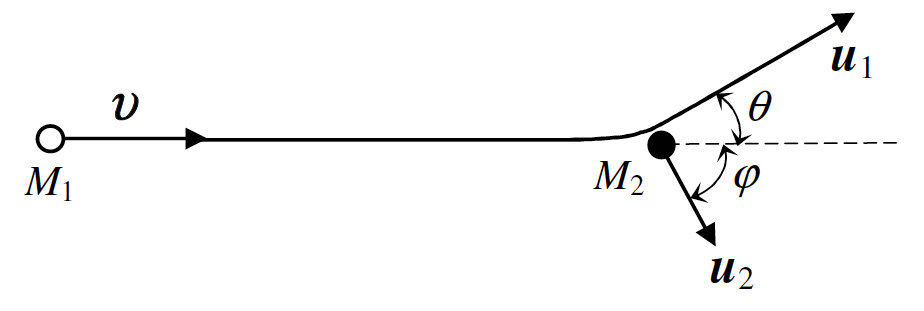
\includegraphics[width=8cm]{picture/nonrelativity/syototu.png}
\caption{実験室系における2体の衝突(\cite{ion}より引用し、一部改変)}
\label{fig:syototu}
\end{figure}

上の図\ref{fig:syototu}において入射粒子の質量を$M_{1}$、反跳粒子の質量を$M_{2}$とする。また、入射粒子の衝突前の速度を$\bm{v}$、衝突後の速度を$\bm{u_{1}}$、反跳粒子の速度を$\bm{u_{2}}$とする。この時、運動量保存とエネルギー保存を考えると、
\begin{equation}
\frac{1}{2}M_{1}v^{2} = \frac{1}{2}M_{1}u_{1}^{2} + \frac{1}{2}M_{2}u_{2}^{2}
\end{equation}
\begin{equation}
M_{1}v = M_{1}u_{1}\cos\theta+M_{2}u_{2}\cos\varphi
\end{equation}
\begin{equation}
0 = M_{1}u_{1}\sin\theta-M_{2}u_{2}\sin\varphi
\end{equation}
が成り立つ。3つの式に対して、4つの未知数$u_{1}$、$u_{2}$、$\theta$、$\varphi$があるので、連立することで以下の関係式が得られる。
\begin{equation}\label{eq:kakudo}
\tan\theta = \frac{M_{2}\sin2\varphi}{M_{1}-M_{2}\cos2\varphi}   
\end{equation}
\begin{equation}
E = \frac{1}{2}M_{1}u_{1}^{2} = \left(\frac{M_{1}\cos\theta + \sqrt{M_{2}^{2} - M_{1}^{2}\sin^2\theta}}{M_{1}+M_{2}}\right)^{2}E_{0}
\label{eq:energy}
\end{equation}
\begin{equation}\label{eq:recoil}
T = \frac{1}{2}M_{2}u_{2}^{2} = \frac{4M_{1}M_{2}}{\left(M_{1}+M_{2}\right)^{2}}E_{0}\cos^2\varphi
\end{equation}
ただし、$E_{0} = \frac{1}{2}M_{1}v^{2}$である。ここで、$E$は散乱陽子のエネルギーである。
また、(\ref{eq:kakudo})~(\ref{eq:recoil})式を $A = \frac{M_{2}}{M_{1}}$を用いて書き直すと、以下のようになる。
\begin{equation}\label{eq:kakudokai}
\tan\theta = \frac{A\sin2\varphi}{1 - A\cos2\varphi}   
\end{equation}
\begin{equation}
E  = \left(\frac{\cos\theta + \sqrt{\cos^2\theta + A^{2} -1}}{A + 1}\right)^{2}E_{0}
\label{eq:energykai}
\end{equation}
\begin{equation}\label{eq:recoilkai}
T = \frac{4A}{\left(A + 1\right)^{2}}E_{0}\cos^2\varphi
\end{equation}

\eqref{eq:energykai}、\eqref{eq:recoilkai}をグラフにすると、図\ref{fig:scaene}、図\ref{fig:recoil}のようになる。ただし、$E_{0}=$\;3\;MeVである。

\begin{figure}[bhtp]
  \begin{minipage}{0.5\hsize}
    \begin{center}
      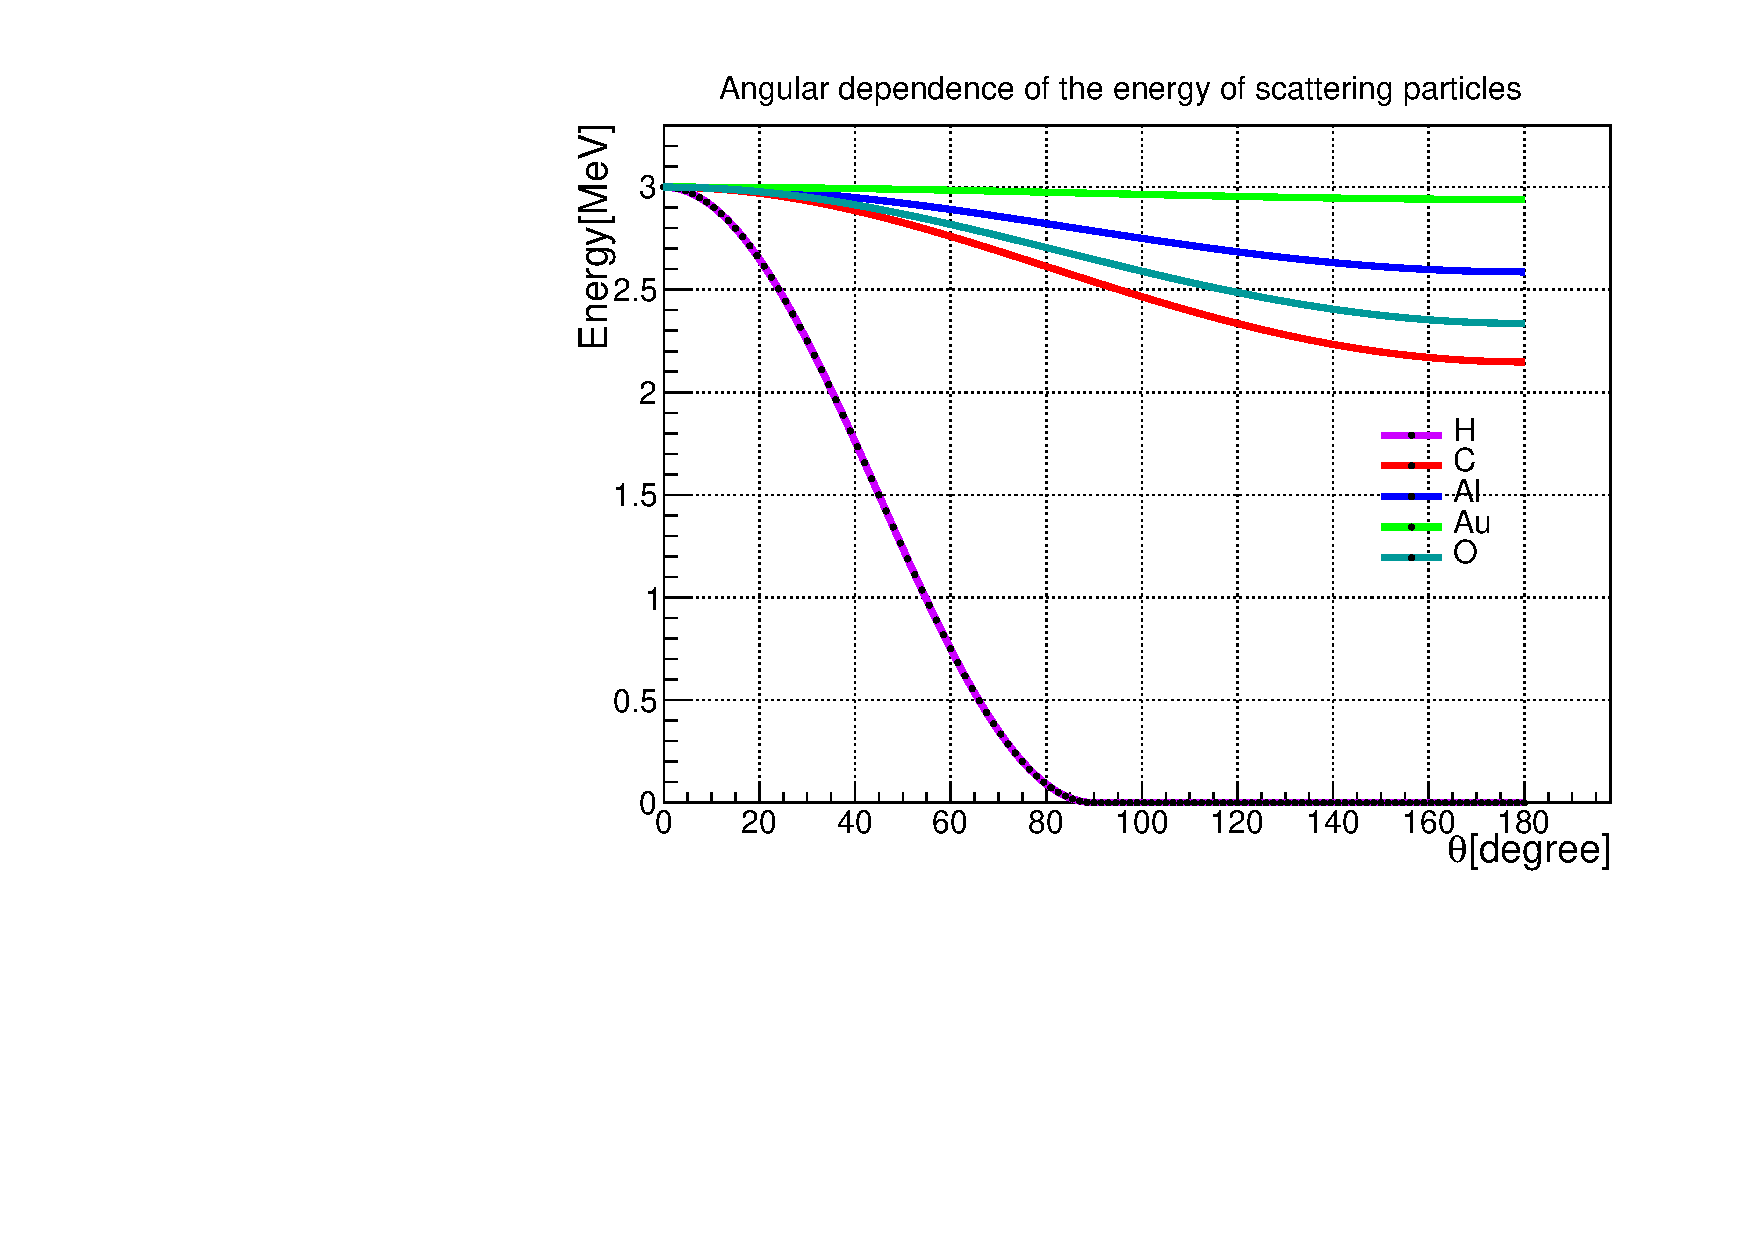
\includegraphics[width=73mm]{picture/nonrelativity/newsca.pdf}
    \end{center}
    \caption{散乱陽子のエネルギー}
    \label{fig:scaene}
  \end{minipage}
  \begin{minipage}{0.5\hsize}
    \begin{center}
      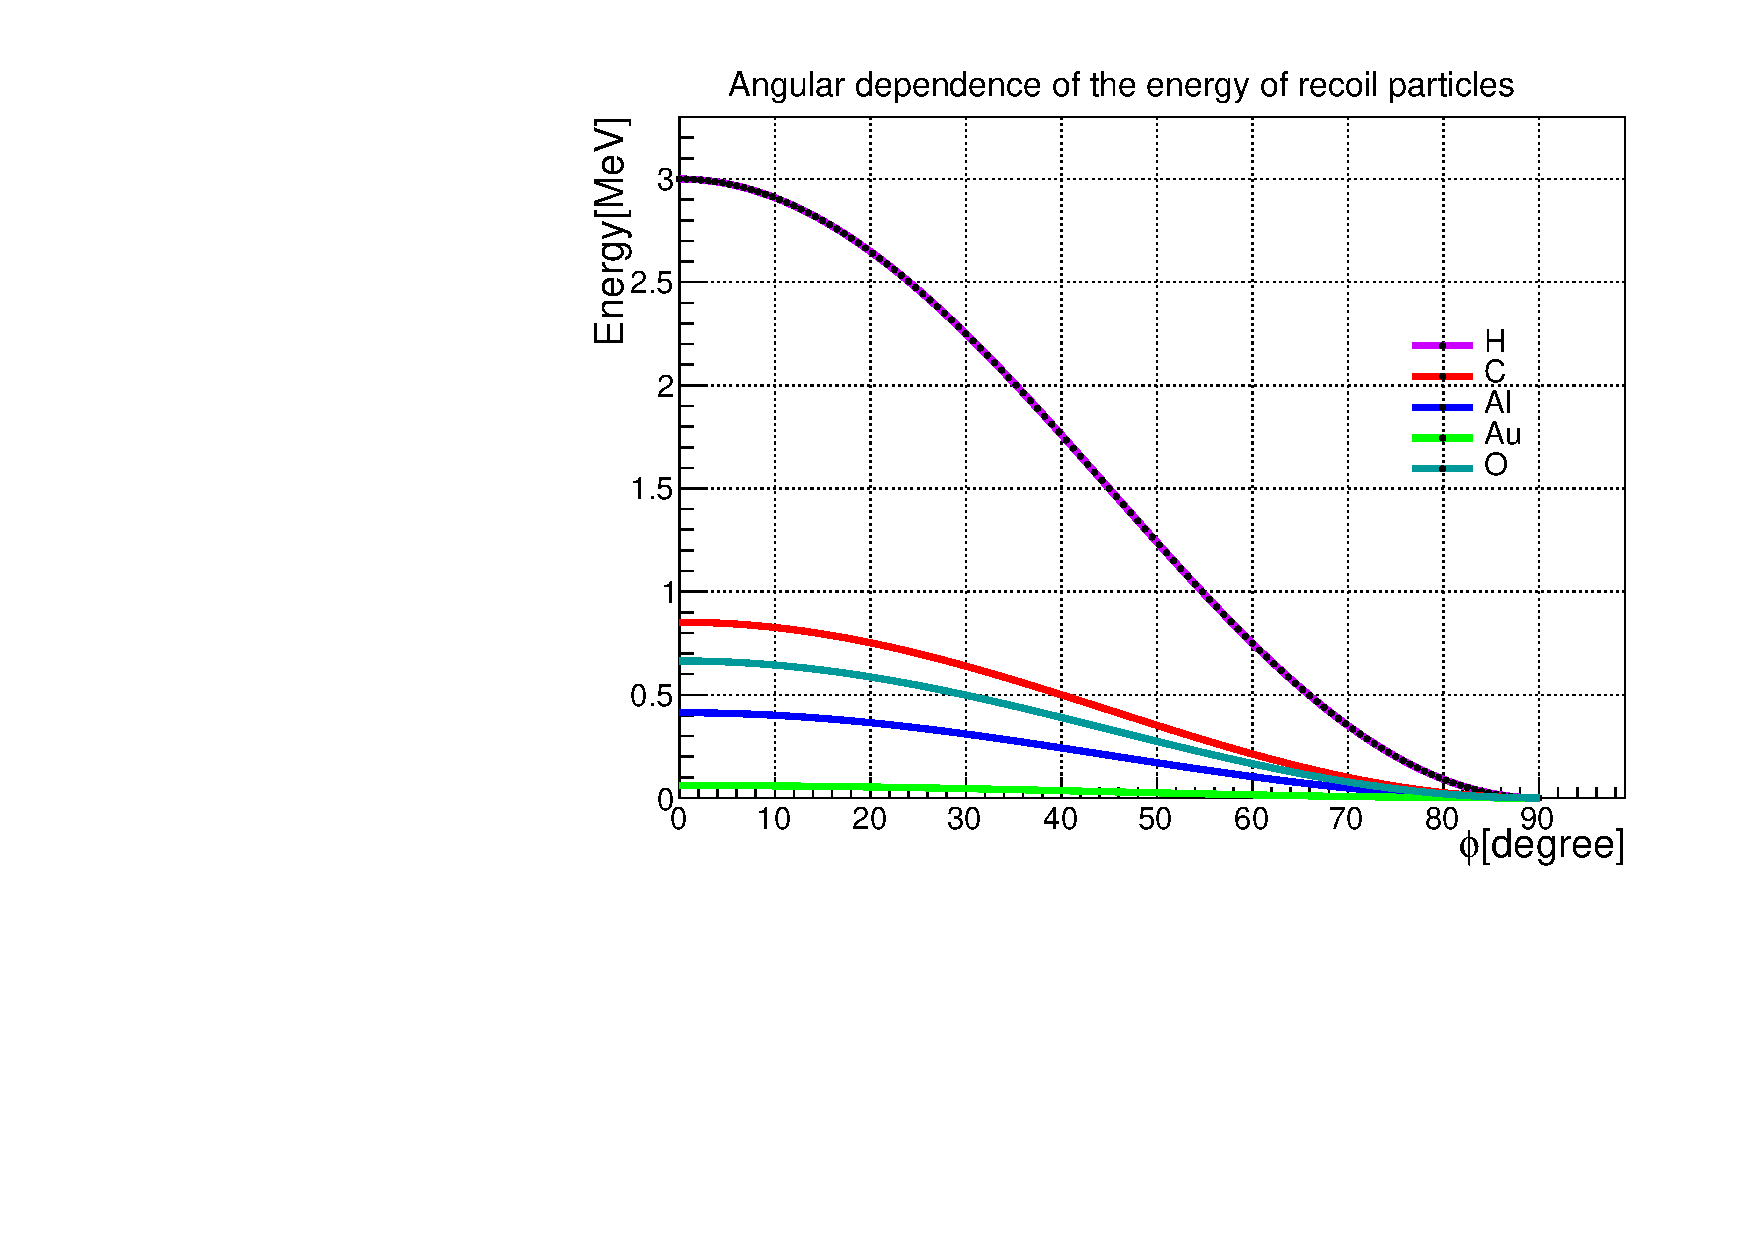
\includegraphics[width=73mm]{picture/nonrelativity/recoil.pdf}
    \end{center}
    \caption{反跳粒子のエネルギー}
    \label{fig:recoil} 
  \end{minipage}
\end{figure}
\newpage
\subsubsection{p-p散乱のopening angle}\label{opening}
次にp-p散乱(陽子-陽子散乱)のopening angleについて考える。

p-p散乱の場合$A = 1$なので、(\ref{eq:kakudokai})式から以下の式が導かれる。
\begin{equation}\label{eq:ten}
\tan\theta = \frac{\sin2\varphi}{1 - \cos2\varphi} =\frac{1}{\tan\varphi}
\end{equation}
(\ref{eq:ten})の方程式を解くことで、
\begin{equation}
\theta + \varphi = 90^{\circ}
\end{equation}
となるので、p-p散乱のopening angleは $90^{\circ}$になる。

\subsubsection{実験室系、重心系間の変換式}
前述の通り微分散乱断面積は重心系で定義されるが、実際には実験室系で測定されるので実験室系における物理量を重心系に変換する必要が出てくる。

後述する相対論の影響がないとすると、実験室系での散乱角$\theta$と重心系での散乱角$\theta_{cm}$の間に成り立つ関係式は、
\begin{equation}
    \tan\theta = \frac{\sin\theta_{cm}}{\cos\theta_{cm}+\frac{1}{n}}\label{eq:henkan1}
\end{equation}
となる\cite{kyodai}。ただし、$n=m_{2}/m_{1}$である。

p-p散乱の場合、$n=1$なので
\begin{equation}
    \theta=\frac{\theta_{cm}}{2}
\end{equation}
が成り立つ。

また、実験室系と重心系における微分散乱断面積をそれぞれ$\left(\frac{d\sigma}{d\Omega}\right)_\text{lab}$,$\left(\frac{d\sigma}{d\Omega}\right)_\text{cm}$とすると、これらの間の関係式は
\begin{equation}
    \left(\frac{d\sigma}{d\Omega}\right)_\text{cm} = \frac{1+\frac{\cos\theta_{cm}}{n}}{\left(1+\frac{2}{n}\cos\theta_{cm}+\frac{1}{n^2}\right)^{\frac{3}{2}}}\left(\frac{d\sigma}{d\Omega}\right)_\text{lab}\label{eq:henkan2}
\end{equation}
で表される\cite{kyodai}。


\end{document}
\documentclass[a4paper,11pt,dvipdfmx]{jsarticle}

\usepackage{bm}
\usepackage[dvipdfmx]{graphicx}
\usepackage[dvipdfmx]{color}
\usepackage{ascmac}
\usepackage{amsmath}
\usepackage{amssymb}
\usepackage{siunitx}
\usepackage{otf}
\usepackage[dvipdfmx]{graphicx}
\pagestyle{plain}
\usepackage{float}
\usepackage[dvipdfmx]{hyperref}
\usepackage{pxjahyper}
\usepackage{here}
\usepackage{titlesec}
\titleformat*{\section}{\LARGE\bfseries}
\titleformat*{\subsection}{\normalsize\bfseries}
\usepackage{url}
\usepackage[table,xcdraw]{xcolor}
\hypersetup{% hyperrefオプションリスト
setpagesize=false,
 bookmarksnumbered=true,%
 bookmarksopen=true,%
 colorlinks=true,%
 linkcolor=blue,
 citecolor=blue,
}

\begin{document}
\renewcommand\thefootnote{\arabic{footnote})}
\newpage
\subsection{相対論の運動学\cite{kyodai}}
本実験では最大でも$\beta=0.08$なので十分非相対論の領域として扱えるが、高エネルギー領域で散乱実験を行う際には相対論で取り扱わなければならない場合もある。本節ではそのような相対論の運動学について議論する。

以下では入射粒子を粒子1、標的粒子を粒子2と呼称する。

図\ref{fig:initial}のように、実験室系において静止している粒子2(質量$m_{2}$)に粒子1(質量$m_{1}$)を打ち込む状況を考える。このとき重心系の始状態における粒子1、2の運動量を$\bm{p}^{cm}$,$-\bm{p}^{cm}$、終状態における粒子1、2の運動量を$\bm{p}^{cm'}$,$-\bm{p}^{cm'}$とし、実験室系の始状態における粒子1の運動量を$\bm{p}_{1}$、終状態における各粒子の運動量を$\bm{p}'_{1}$,\,$\bm{p}'_{2}$とする。散乱がxy平面上で起こるという仮定の下で実験室系と重心系における4元運動量の保存則を考えると、次頁の式\eqref{eq:yogen1},\eqref{eq:yogen2}が成り立つ。
\\
\\
\\
\begin{figure}[htbp]
\centering
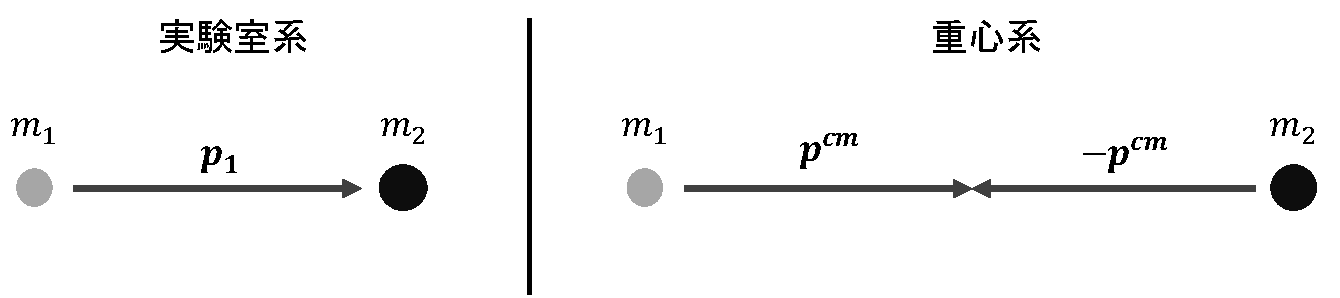
\includegraphics[width=12cm]{picture/relativity/initial.pdf}
\caption{始状態}
\label{fig:initial}
\end{figure}
\\
\\
\begin{figure}[htbp]
\centering
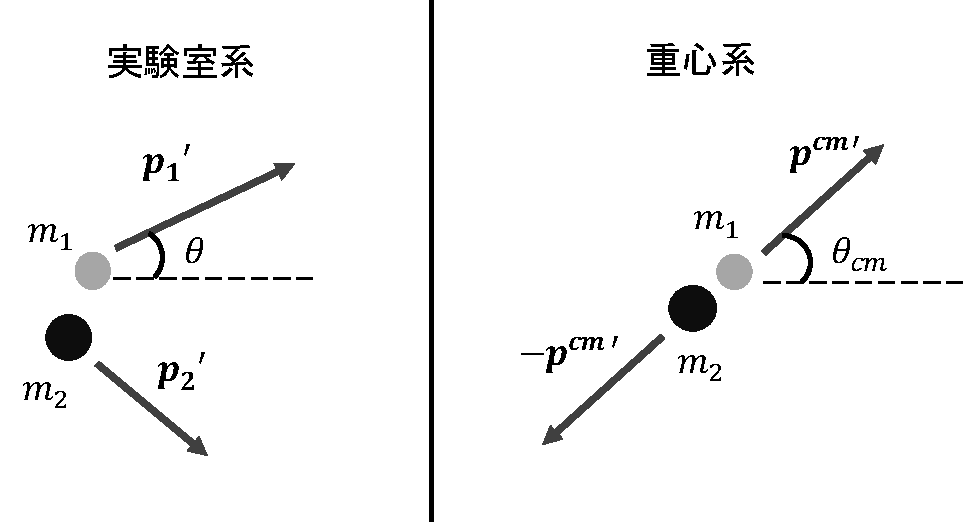
\includegraphics[width=9cm]{picture/relativity/final1.pdf}
\caption{終状態}
\label{fig:final}
\end{figure}
\newpage
\begin{equation}
    \left(
    \begin{array}{c}
     \frac{\varepsilon_{1}}{c}  \\
      p_{1}\\
      0 \\
      0
    \end{array}
  \right)  + \left(
    \begin{array}{c}
      m_{2}c \\
      0\\
      0 \\
      0
    \end{array}
  \right)=
      \left(
    \begin{array}{c}
     \frac{\varepsilon'_{1}}{c}  \\
      p'_{1x}\\
      p'_{1y}\\
      0
    \end{array}
  \right) +
    \left(
    \begin{array}{c}
     \frac{\varepsilon'_{2}}{c}  \\
      p'_{2x}\\
      p'_{2y}\\
      0
    \end{array}
  \right) \label{eq:yogen1}
\end{equation}
\begin{equation}
    \left(
    \begin{array}{c}
     \frac{\varepsilon_{1}^{cm}}{c}  \\
      p^{cm}\\
      0 \\
      0
    \end{array}
  \right)  + \left(
    \begin{array}{c}
      \frac{\varepsilon_{2}^{cm}}{c}  \\
      -p^{cm}\\
      0 \\
      0
    \end{array}
  \right)=
      \left(
    \begin{array}{c}
     \frac{\varepsilon^{cm'}_{1}}{c}  \\
      p^{cm'}_{x}\\
      p^{cm'}_{y}\\
      0
    \end{array}
  \right) +
    \left(
    \begin{array}{c}
     \frac{\varepsilon^{cm'}_{2}}{c}  \\
      -p^{cm'}_{x}\\
      -p^{cm'}_{y}\\
      0
    \end{array}
  \right) \label{eq:yogen2}
\end{equation}

また、この散乱は弾性散乱であり、
\begin{equation}
   s=\left(\frac{\varepsilon}{c}\right)^2-p^2=(mc)^2
\end{equation}
で表される$s$は散乱の前後で保存されるので、各粒子における$s$の保存より、
\begin{align}
     \left(\frac{\varepsilon'_{1}}{c}\right)^2-(\bm{p}'_{1})^2 = \left(\frac{\varepsilon^{cm}_{1}}{c}\right)^2-(\bm{p}^{cm})^2 =\left(\frac{\varepsilon^{cm'}_{1}}{c}\right)^2-(\bm{p}^{cm'})^2 \notag\\*
     =\left(\frac{\varepsilon_{1}}{c}\right)^2-(\bm{p}_{1})^2 = (m_{1}c)^2 \label{eq:snohozon}
\end{align}
\begin{equation}
    \left(\frac{\varepsilon'_{2}}{c}\right)^2-(\bm{p}'_{2})^2 = \left(\frac{\varepsilon^{cm}_{2}}{c}\right)^2-(\bm{p}^{cm})^2= 
     \left(\frac{\varepsilon^{cm'}_{2}}{c}\right)^2-(\bm{p}^{cm'})^2 =
     (m_{2}c)^2
\end{equation}

また、4元運動量の保存より
\begin{alignat}{3}
    \frac{\varepsilon^{cm}_{1}}{c} &= \frac{\varepsilon^{cm'}_{1}}{c}, &\qquad \frac{\varepsilon^{cm}_{2}}{c} &= \frac{\varepsilon^{cm'}_{2}}{c}, & \qquad 
    |\bm{p}^{cm}|&=|\bm{p}^{cm'}|
\end{alignat}
が言える。
次に、重心系での全エネルギーを$E^{cm}$とすると、始状態における全系のローレンツ不変量から、
\begin{equation*}
    \left(\frac{E^{cm}}{c}\right)^2 - 0 = \left(\frac{\varepsilon_{1}}{c} + m_{2}c\right)^{2} -(\bm{p_{1}})^2
\end{equation*}
\begin{equation}
   \therefore \left(\frac{E^{cm}}{c}\right)^2 = (m_{1}c)^{2} + (m_{2}c)^{2} + 2\frac{\varepsilon_{1}}{c}m_{2}c \qquad (\,\because\eqref{eq:snohozon})
\end{equation}

次にローレンツ変換のパラメータ$\beta$を求める。始状態の全系の変換は
\begin{equation}
    \left(
    \begin{array}{c}
     \frac{\varepsilon_{1}}{c} +m_{2}c \\
      p_{1}\\
      0 \\
      0
    \end{array}
  \right)  = \left(
    \begin{array}{cccc}
      \gamma & \beta\gamma & 0 & 0 \\
      \beta\gamma & \gamma & 0 & 0 \\
      0 & 0 & 1 & 0 \\
      0 & 0 & 0 & 1
    \end{array}
    \right) 
      \left(
    \begin{array}{c}
     \frac{E^{cm}}{c}  \\
      0\\
      0\\
      0
    \end{array}
  \right) =
    \left(
    \begin{array}{c}
     \gamma\frac{E^{cm}}{c}  \\
      \beta\gamma\frac{E^{cm}}{c}\\
      0\\
      0
    \end{array}
  \right) 
\end{equation}
\begin{equation}
    \therefore \gamma=\frac{\frac{\varepsilon_{1}}{c} +m_{2}c}{\frac{E^{cm}}{c}}
\end{equation}
また\;$\gamma=1/\sqrt{1-\beta^2}$より、
\begin{equation}
    \beta=\frac{\sqrt{\gamma^{2}-1}}{\gamma}=\frac{\sqrt{\left(\frac{\varepsilon_{1}}{c}\right)^2-(m_{1}c)^2}}{\frac{\varepsilon_{1}}{c} +m_{2}c}=\frac{p_{1}}{\frac{\varepsilon_{1}}{c} +m_{2}c}
\end{equation}
となる。
次に始状態、終状態それぞれにおける粒子1についての変換から、
\begin{equation}
    \left(
    \begin{array}{c}
     \frac{\varepsilon^{cm}_{1}}{c}  \\
      p^{cm}\\
      0 \\
      0
    \end{array}
  \right)  = \left(
    \begin{array}{cccc}
      \gamma & -\beta\gamma & 0 & 0 \\
      -\beta\gamma & \gamma & 0 & 0 \\
      0 & 0 & 1 & 0 \\
      0 & 0 & 0 & 1
    \end{array}
    \right) 
      \left(
    \begin{array}{c}
     \frac{\varepsilon_{1}}{c}  \\
      p_{1}\\
      0\\
      0
    \end{array}
  \right) =
    \left(
    \begin{array}{c}
     \gamma\left(\frac{\varepsilon_{1}}{c} -\beta p_{1}\right)  \\
      \gamma\left(p_{1}-\beta\frac{\varepsilon_{1}}{c}\right)\\
      0\\
      0
    \end{array}
  \right) 
\end{equation}
\begin{equation}
    \left(
    \begin{array}{c}
     \frac{\varepsilon'_{1}}{c}  \\
      p'_{1x}\\
      p'_{1y} \\
      0
    \end{array}
  \right)  = \left(
    \begin{array}{cccc}
      \gamma & \beta\gamma & 0 & 0 \\
      \beta\gamma & \gamma & 0 & 0 \\
      0 & 0 & 1 & 0 \\
      0 & 0 & 0 & 1
    \end{array}
    \right) 
      \left(
    \begin{array}{c}
     \frac{\varepsilon^{cm'}_{1}}{c}  \\
      p^{cm'}_{x}\\
      p^{cm'}_{y}\\
      0
    \end{array}
  \right) =
    \left(
    \begin{array}{c}
     \gamma\left(\frac{\varepsilon^{cm'}_{1}}{c} +\beta p^{cm'}_{x}\right)  \\
      \gamma\left(p^{cm'}_{x}+\beta\frac{\varepsilon^{cm'}_{1}}{c}\right)\\
      p^{cm'}_{y}\\
      0
    \end{array}
  \right) 
\end{equation}
よって、
\begin{align}
    \frac{p'_{1x}}{\gamma} &= p^{cm'}_{x}+ \beta\frac{\varepsilon^{cm'}_{1}}{c} = p^{cm'}_{x}+ \beta\frac{\varepsilon^{cm}_{1}}{c} \notag\\
    &= p^{cm'}_{x} + \beta\gamma\left(\frac{\varepsilon_{1}}{c}-\beta p_{1}\right) \notag\\
    &= p^{cm'}_{x} + \left[\frac{\frac{\varepsilon_{1}}{c}\left(\frac{\varepsilon_{1}}{c}+m_{2}c\right)}{\left(\frac{E^{cm}}{c}\right)^2}-\frac{\left(\frac{\varepsilon_{1}}{c}\right)^2-(m_{1}c)^2}{\left(\frac{E^{cm}}{c}\right)^2}\right]\frac{p_{1}}{\gamma} \notag\\
    &=  p^{cm'}_{x} +\frac{\frac{\varepsilon_{1}}{c}m_{2}c+(m_{1}c)^2}{\left(\frac{E^{cm}}{c}\right)^2}\frac{p_{1}}{\gamma} 
\end{align}
ここで、$x$成分のみを$\tfrac{1}{\gamma}$倍したベクトルを「$\;\Bar{}\;$」をつけて表すと、
\begin{alignat*}{2}
    \Bar{\bm{p}'_{1}} &= \left(\frac{p'_{1x}}{\gamma} \quad p'_{1y} \quad 0\right), &\quad  \Bar{\bm{p}_{1}} &= \left(\frac{p_{1x}}{\gamma} \quad 0 \quad 0\right) 
\end{alignat*}
であり、
\begin{equation}
     \Bar{\bm{p}'_{1}} = \bm{p}^{cm'} +\frac{\frac{\varepsilon_{1}}{c}m_{2}c+(m_{1}c)^2}{\left(\frac{E^{cm}}{c}\right)^2}\Bar{\bm{p}_{1}}\label{eq:p1}
\end{equation}
が成り立つ。粒子2についても同様に、
\begin{equation}
    \left(
    \begin{array}{c}
     \frac{\varepsilon^{cm}_{2}}{c}  \\
      -p^{cm}\\
      0 \\
      0
    \end{array}
  \right)  = \left(
    \begin{array}{cccc}
      \gamma & -\beta\gamma & 0 & 0 \\
      -\beta\gamma & \gamma & 0 & 0 \\
      0 & 0 & 1 & 0 \\
      0 & 0 & 0 & 1
    \end{array}
    \right) 
      \left(
    \begin{array}{c}
     m_{2}c\\
      0\\
      0\\
      0
    \end{array}
  \right) =
    \left(
    \begin{array}{c}
     \gamma m_{2}c\\
      -\beta\gamma m_{2}c\\
      0\\
      0
    \end{array}
  \right) 
\end{equation}
\begin{equation}
    \left(
    \begin{array}{c}
     \frac{\varepsilon'_{2}}{c}  \\
      p'_{2x}\\
      p'_{2y} \\
      0
    \end{array}
  \right)  = \left(
    \begin{array}{cccc}
      \gamma & \beta\gamma & 0 & 0 \\
      \beta\gamma & \gamma & 0 & 0 \\
      0 & 0 & 1 & 0 \\
      0 & 0 & 0 & 1
    \end{array}
    \right) 
      \left(
    \begin{array}{c}
     \frac{\varepsilon^{cm'}_{2}}{c}  \\
      -p^{cm'}_{x}\\
      -p^{cm'}_{y}\\
      0
    \end{array}
  \right) =
    \left(
    \begin{array}{c}
     \gamma\left(\frac{\varepsilon^{cm'}_{2}}{c} -\beta p^{cm'}_{x}\right)  \\
      \gamma\left(-p^{cm'}_{x}+\beta\frac{\varepsilon^{cm'}_{2}}{c}\right)\\
      -p^{cm'}_{y}\\
      0
    \end{array}
  \right) 
\end{equation}
より
\begin{align}
    \frac{p'_{2x}}{\gamma} &= -p^{cm'}_{x}+ \beta\frac{\varepsilon^{cm'}_{2}}{c} = -p^{cm'}_{x}+ \beta\frac{\varepsilon^{cm}_{2}}{c} \notag\\
    &= -p^{cm'}_{x} + \beta\gamma m_{2}c \notag\\
    &= -p^{cm'}_{x} +\frac{\left(\frac{\varepsilon_{1}}{c}+m_{2}c\right)m_{2}c}{\left(\frac{E^{cm}}{c}\right)^2}\frac{p_{1}}{\gamma} 
\end{align}
だから、
\begin{equation*}
    \Bar{\bm{p}'_{2}} = \left(\frac{p'_{2x}}{\gamma} \quad p'_{2y} \quad 0\right)
\end{equation*}
として
\begin{equation}
     \Bar{\bm{p}'_{2}} = -\bm{p}^{cm'} +\frac{\left(\frac{\varepsilon_{1}}{c}+m_{2}c\right)m_{2}c}{\left(\frac{E^{cm}}{c}\right)^2}\Bar{\bm{p}_{1}}\label{eq:p2}
\end{equation}
となる。

ここで、 $\Bar{\bm{p}_{1}}$と$\Bar{\bm{p}'_{1}}$ のなす角を$\Bar{\theta}$とすると、
\begin{equation}
    \tan\Bar{\theta}=\frac{p'_{1y}}{p'_{1x}/\gamma}=\gamma\tan\theta \label{eq:bartheta}
\end{equation}
また、$n=\left(\frac{\varepsilon_{1}}{c}m_{2}c + (m_{2}c)^2\right)/\left(\frac{\varepsilon_{1}}{c}m_{2}c + (m_{1}c)^2\right)$とすれば以前の結果を用いて、
\begin{equation}
    \tan\Bar{\theta} = \frac{\sin\theta_{cm}}{\cos\theta_{cm}+\frac{1}{n}} \label{eq:barcm}
\end{equation}
となる。
よって、式\eqref{eq:bartheta}と\eqref{eq:barcm}より
\begin{equation}
    \tan\theta = \frac{\sin\theta_{cm}}{\gamma\left(\cos\theta_{cm}+\frac{1}{n}\right)} \label{eq:henkan3}
\end{equation}
これが相対論における実験室系での散乱角$\theta$と重心系での散乱角$\theta_{cm}$を関係づける式である。

例えばp-p散乱の場合、$m_{1}=m_{2}$より$n=1$となり、式\eqref{eq:barcm}から
\begin{equation}
    \Bar{\theta}=\frac{\theta_{cm}}{2}
\end{equation}
となる。よって、
\begin{equation}
    \theta=\arctan\left(\frac{\tan\frac{\theta_{cm}}{2}}{\gamma}\right)
\end{equation}
となる。

また、実験室系と重心系における微分散乱断面積をそれぞれ$\left(\frac{d\sigma}{d\Omega}\right)_\text{lab}$,$\left(\frac{d\sigma}{d\Omega}\right)_\text{cm}$とすると、これらの間の関係式は、相対論の効果を考慮すると
\begin{equation}
    \left(\frac{d\sigma}{d\Omega}\right)_\text{cm} = \frac{\gamma\left(1+\frac{\cos\theta_{cm}}{n}\right)}{\left(\sin^2\theta_{cm}+\gamma^2\left(\cos\theta_{cm}+\frac{1}{n}\right)^2\right)^{\frac{3}{2}}}\left(\frac{d\sigma}{d\Omega}\right)_\text{lab}\label{eq:henkan4}
\end{equation}
と書ける。

以上から、相対論を考慮する場合は非相対論の変換式\eqref{eq:henkan1},\eqref{eq:henkan2}はそれぞれ\eqref{eq:henkan3},\eqref{eq:henkan4}に変化することがわかる。

\end{document}
\documentclass[a4paper,11pt,dvipdfmx]{jsarticle}

\usepackage{bm}
\usepackage[dvipdfmx]{graphicx}
\usepackage[dvipdfmx]{color}
\usepackage{ascmac}
\usepackage{amsmath}
\usepackage{amssymb}
\usepackage{siunitx}
\usepackage{otf}
\usepackage[dvipdfmx]{graphicx}
\pagestyle{plain}
\usepackage{float}
\usepackage[dvipdfmx]{hyperref}
\usepackage{pxjahyper}
\usepackage{here}
\usepackage{titlesec}
\titleformat*{\section}{\LARGE\bfseries}
\titleformat*{\subsection}{\normalsize\bfseries}
\usepackage{url}
\usepackage[table,xcdraw]{xcolor}
\hypersetup{% hyperrefオプションリスト
setpagesize=false,
 bookmarksnumbered=true,%
 bookmarksopen=true,%
 colorlinks=true,%
 linkcolor=blue,
 citecolor=blue,
}

\begin{document}
\renewcommand\thefootnote{\arabic{footnote})}
\subsection{用いる標的とエネルギー損失}
\label{tarandloss}
ラザフォードの散乱公式より、微分散乱断面積は標的の原子番号に依存することがわかる。今回の実験ではポリエチレン(PE)、金の2種類の標的を使用した。

実験で用いる標的には厚さがあるため、入射陽子及び反跳粒子に対して標的内でのエネルギー損失を考える必要がある。そこで、本節では以下のBethe-Blochの式\eqref{eq:bethe}\cite{introto}を用いて標的内でのエネルギー損失が元の入射陽子のエネルギー$E=$\;3\;MeV\;の$5\%$未満になる厚さを算出する。
\begin{equation}
    -\frac{1}{\rho}\frac{dE}{dx}=K\frac{Z}{A}\frac{1}{\beta^2}\left[\ln\left(\frac{2m_{e}c^2\beta^2}{I\left(1-\beta^2\right)}\right)-\beta^2\right]\label{eq:bethe}
\end{equation}

式\eqref{eq:bethe}の各パラメータは以下の通り。
\begin{alignat*}{3}
    K &= \frac{4\pi N_{A}}{m_{e}c^2}\cdot\left(\frac{e^2}{4\pi\varepsilon_{0}}\right)^{2} \sim0.3071\;[\text{MeV}\cdot\text{cm}^2\cdot\text{g}^{-1}], & \;\; m_{e}c^2 &= 0.511\;[\text{MeV}]
\end{alignat*}
\centerline{$I\;$:平均イオン化エネルギー[MeV],\;\;$Z\;$:標的原子核の原子番号,\;\;$A\;$:標的原子核の質量数,}\\
\centerline{$N_{A}$:アボガドロ定数,\;\;$\rho\;$:標的の密度[g/{cm}$^3$],\;\;$\beta=v(陽子の速度)/c$ }




\begin{table}[htbp]
 \centering
  \begin{tabular}{ccc}
   \hline 
   \  & \,理論値($\mu$m)  & \;\,実験値($\mu$m)  \\
   \hline \hline
   ポリエチレン & 14.0 & 11.5  \\
   金 & 1.91 & 0.17  \\
   \hline    
  \end{tabular}
  \caption{標的の厚さ}
   \label{table:loss}
\end{table}

$E=$\;3\;MeV\;の陽子を用いるとき、$\beta=0.08$であることに注意すると、$5\%$未満になる標的の厚さと実際の厚さは表\ref{table:loss}のように示される。

なおポリエチレンの$\tfrac{dE}{dx}$を考える際は、構成元素の重量比も加味して\cite{eneloss}
\begin{equation}
    \left(\frac{dE}{dx}\right)_{total}=\frac{12}{14}\left(\frac{dE}{dx}\right)_\text{C} + \frac{2}{14}\left(\frac{dE}{dx}\right)_\text{H}
    \label{eq:dedxtot}
\end{equation}
とした。
式\eqref{eq:dedxtot}右辺の添字付きの$\tfrac{dE}{dx}$は、各元素単体で考えたときのエネルギー損失を表している。

\end{document}
\documentclass[a4paper,11pt,dvipdfmx]{jsarticle}

\usepackage{bm}
\usepackage[dvipdfmx]{graphicx}
\usepackage[dvipdfmx]{color}
\usepackage{ascmac}
\usepackage{siunitx}
\usepackage{otf}
\pagestyle{plain}
\usepackage{float}
\usepackage[dvipdfmx]{hyperref}
\usepackage{pxjahyper}
\usepackage{here}
\usepackage{titlesec}
\titleformat*{\section}{\LARGE\bfseries}
\titleformat*{\subsection}{\normalsize\bfseries}
\usepackage{url}
\usepackage[table,xcdraw]{xcolor}
\hypersetup{% hyperrefオプションリスト
setpagesize=false,
 bookmarksnumbered=true,%
 bookmarksopen=true,%
 colorlinks=true,%
 linkcolor=blue,
 citecolor=blue,
}


\begin{document}
\newpage
\section{\LARGE{実験装置(担当:大谷)}}

\subsection{加速器}
今回の実験は、神戸大学深江キャンパスの敷地内にあるタンデム静電加速器を用いて行った。ペレットチェーンに電荷を乗せて高電圧ターミナルに運び上げ高電圧を発生させてイオンを加速する装置で、一つの高電圧で加速イオンの電荷を負から正へ変換して2回加速する装置を総称してタンデム加速器という。\cite{tandemu}タンデム加速器を用いて計測を行ったのは2020年1月4日$\sim$2020年1月11日である。今回の実験では最大エネルギー3MeVの陽子ビームを利用する。表\ref{aclgaiyou}に加速器の使用を、図\ref{aclphoto}に加速器の写真を、図\ref{aclkouzou}に加速器の構図を示す。

\begin{figure}[H]
    \centering
    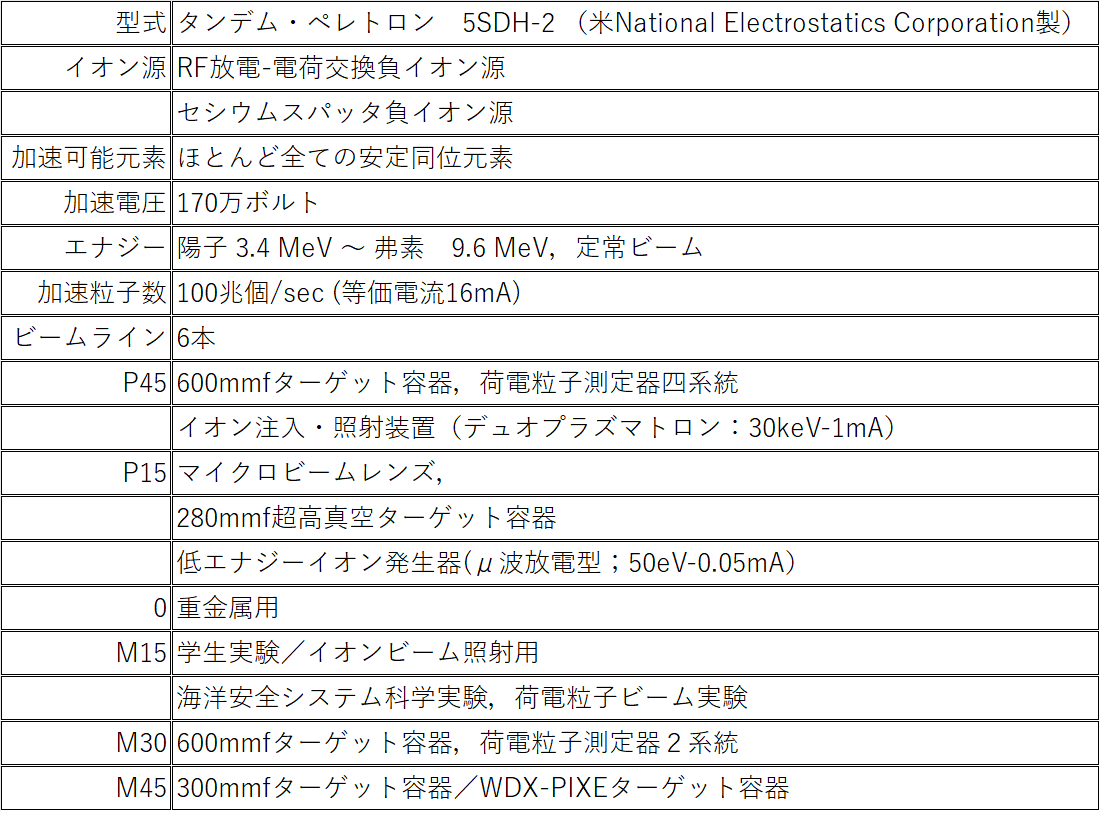
\includegraphics[width=90mm]{picture/setup/aclgaiyou.png}
    \caption{加速器の概要\cite{kasokukishiyou}}
    \label{aclgaiyou}
\end{figure}

\begin{figure}[H]
    \centering
    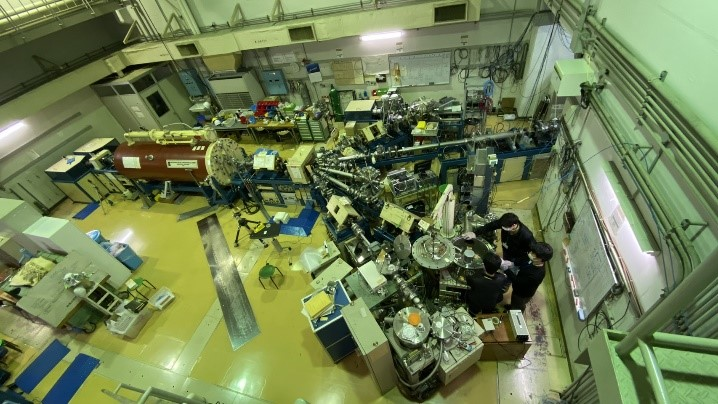
\includegraphics[width=90mm]{picture/setup/aclphoto.jpg}
    \caption{加速器の写真}
    \label{aclphoto}
\end{figure}

\begin{figure}[H]
    \centering
    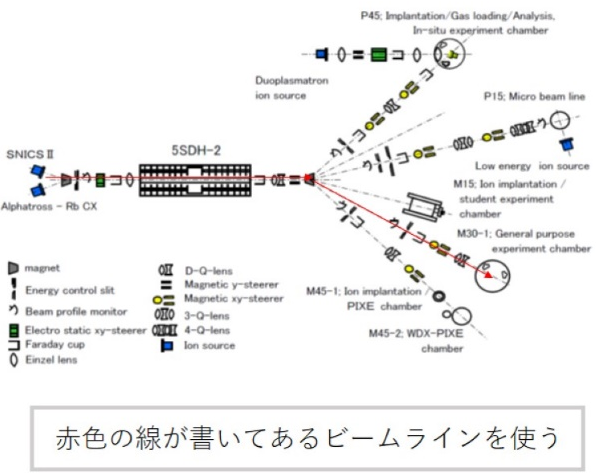
\includegraphics[width=80mm]{picture/setup/aclkouzou.png}
    \caption{加速器の構造\cite{beam}}
    \label{aclkouzou}
\end{figure}

\subsubsection{加速器本体}
加速器本体は、直径1.07m、長さ3.94mの円柱型である。負イオン源では原子に電子を結合させ負イオンを生成する。これを加速するため超高真空に保たれた初段加速管に入射し負イオン加速管入口まで到達させる。生成した負イオンは加速器タンクに入射し、タンク中央の正の電位を持った1.5MVの高電圧ターミナルと入射電極との電位差によって生成した電界によって加速される。このとき負イオンは1.5MeVに加速される。高電圧ターミナルに到達した負イオンは電子ストリッパー(窒素ガス層)で多数の電子がはぎ取られ正イオン(陽子)に変換される。生成した陽子は高電圧ターミナルと出口電極の間に生成した電界により再び加速される。ここで陽子はさらに1.5MeVに加速され、合計3MeVのエネルギーを持った陽子ビームとなる。加速されたビームは、二連四重極磁石によって収束された後、分析・振分電磁石により各ビームラインに偏光される。図\ref{aclmoshi}に加速器本体の模式図を示す。\cite{syousen}

\begin{figure}[H]
    \centering
    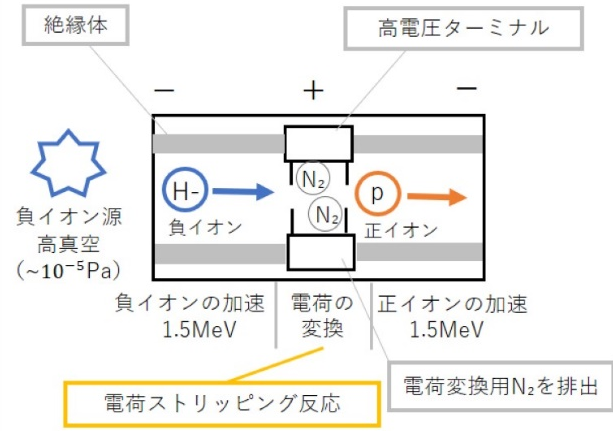
\includegraphics[width=70mm]{picture/setup/aclhonmoshi.png}
    \caption{加速器本体の模式図}
    \label{aclmoshi}
\end{figure}

\end{document}
\documentclass[a4paper,11pt,dvipdfmx]{jsarticle}

\usepackage{bm}
\usepackage[dvipdfmx]{graphicx}
\usepackage[subrefformat=parens]{subcaption}
\usepackage[dvipdfmx]{color}
\usepackage{ascmac}
\usepackage{siunitx}
\usepackage{otf}
\pagestyle{plain}
\usepackage{float}
\usepackage[dvipdfmx]{hyperref}
\usepackage{pxjahyper}
\usepackage{here}
\usepackage{titlesec}
\titleformat*{\section}{\LARGE\bfseries}
\titleformat*{\subsection}{\normalsize\bfseries}
\usepackage{url}
\usepackage{comment}
\usepackage[table,xcdraw]{xcolor}
\hypersetup{% hyperrefオプションリスト
setpagesize=false,
 bookmarksnumbered=true,%
 bookmarksopen=true,%
 colorlinks=true,%
 linkcolor=blue,
 citecolor=blue,
}

\begin{document}


\subsection{セットアップ}


\subsubsection{真空チェンバー}
加速器から送られてきた陽子ビームは、真空チェンバー内に誘導しターゲットに衝突させる。真空チェンバーの写真を図\ref{chanber}に、真空チェンバー内の模式図を図\ref{chanbermoshi}に示す。ターゲットは、アルミ板に張り付け又は挟まれて設置されている。真ん中にある円柱管は二次電子抑制管である。検出器には2.3節で記載するPINフォトダイオードをチャージアンプに付けたものをPINフォト台に設置し利用する。今回の研究では散乱陽子と反跳粒子の両方を検出したいため、検出器を2つ設置した。図\ref{chanbermoshi}の赤矢印のように加速器で加速した陽子を真空チェンバー内に誘導し、ターゲットに衝突させる。二次電子抑制管とビームストッパーは導通しており、電流値を測定することが出来る。また、ターゲットホルダーに当たったビームによる電流値も測定できるようになっている。真空チェンバーは真空ポンプに接続されており、10$^\text{-5}$Paの真空状態を作れるようになっている。
 
 
  \begin{figure}[H]
    \centering
    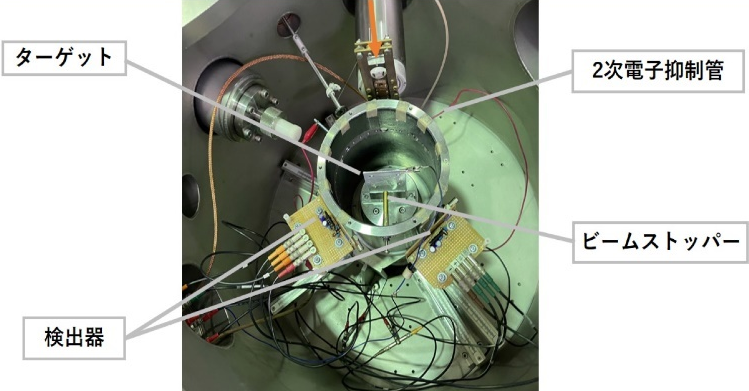
\includegraphics[width=80mm]{picture/setup/chanber.png}
    \caption{真空チェンバーの写真}
    \label{chanber}
  \end{figure}
  
  \begin{figure}[H]
    \centering
    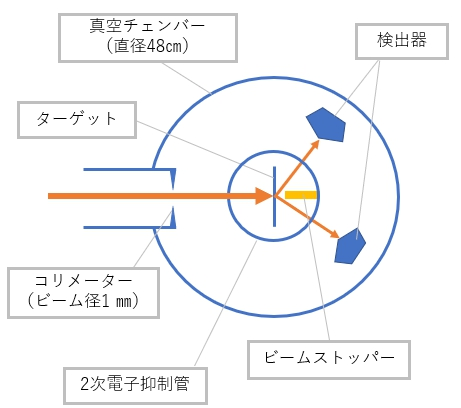
\includegraphics[width=70mm]{picture/setup/chanbermoshi.jpg}
    \caption{真空チェンバー内の模式図}
    \label{chanbermoshi}
  \end{figure}
  
\subsubsection{二次電子抑制管}
真空チェンバーの真ん中にある円柱管を二次電子抑制管という。二次電子抑制管の直径は12cmであり、10度ごとに直径3mmのネジ穴があいている。そのため10度ずつ検出器を動かして実験を行うことができる。今回利用する二次電子抑制管には、ビームストッパーの位置を軸として45度の部分に穴が開いていたため、測定の際の40度・50度への影響を考えてネジで穴を塞いでいる。また140度の穴は大きいものになっている。図\ref{yokokan}に横から見た二次電子抑制管の写真を示す。
 
  \begin{figure}[H]
    \centering
    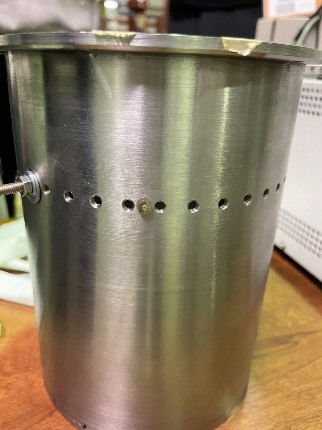
\includegraphics[width=35mm]{picture/setup/yokokan.jpg}
    \caption{横から見た二次電子抑制管の写真}
    \label{yokokan}
  \end{figure}
  
\subsubsection{ビームストッパー}
ラザフォード散乱の微分散乱断面積は、散乱の角度が小さくなるにつれて急速に増大する。そのため、散乱角$\theta=30^{\circ}$未満の散乱が二次電子抑制管で再び散乱してしまうと大きなバックグラウンドになりかねない。これを防ぐためにビームストッパーを設置する。

\par
ビームストッパーは市販の真鍮パイプを切断したものであり、これにネジを付け2次電子抑制管に設置する。長さは43mm、内径は4.5mm、厚さは1mmである。利用したビームストッパーは先行研究\cite{2019}で実績が証明されていたものを利用している。図\ref{stphoto}にビームストッパーの写真を、図\ref{stsekkei}にビームストッパーの設計図を示す。ビームストッパーは真鍮製で、厚さが1mmあるため、図\ref{stmoshi1}のようにビームを十分に止めることが出来る。図\ref{stmoshi2}のようにねじで反射したとしても、反射したビームの反射角は約3度になるため今回の測定範囲に関しては影響がない。

\begin{figure}[H]
 \begin{minipage}{0.5\hsize}
  \begin{center}
   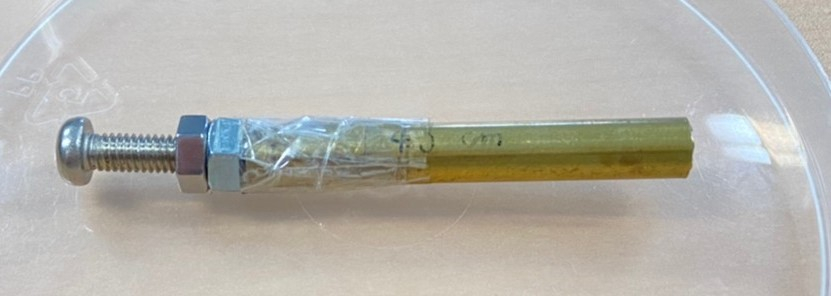
\includegraphics[width=50mm]{picture/setup/stopperphoto.jpg}
  \end{center}
  \caption{ビームストッパーの写真}
  \label{stphoto}
 \end{minipage}
 \begin{minipage}{0.5\hsize}
  \begin{center}
   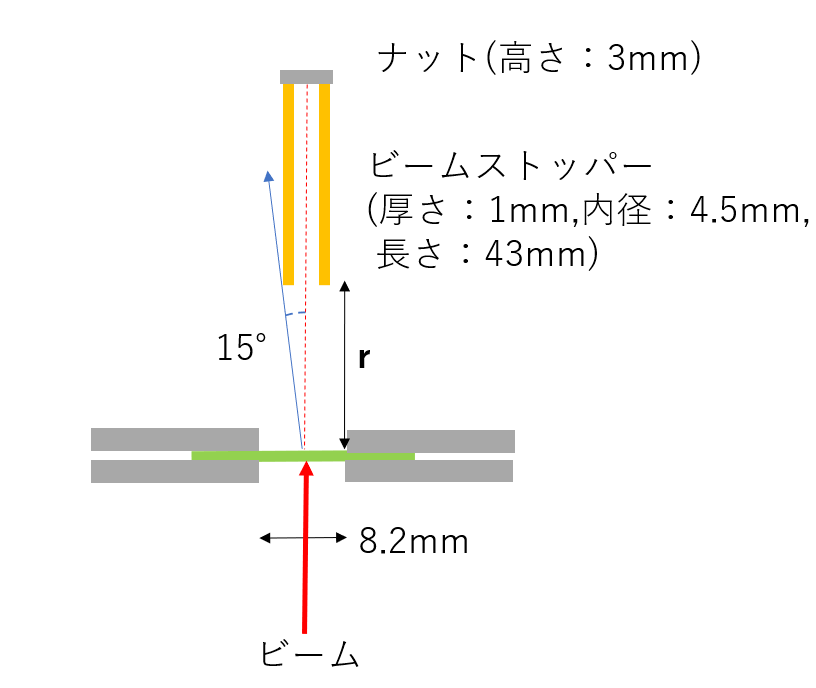
\includegraphics[width=40mm]{picture/setup/stoppersekkei.png}
  \end{center}
  \caption{ビームストッパーの設計図\cite{2019}}
  \label{stsekkei}
 \end{minipage}
\end{figure}

\begin{figure}[H]
  \begin{minipage}{0.5\hsize}
    \centering
    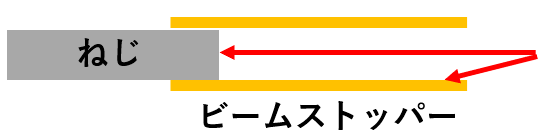
\includegraphics[width=50mm]{picture/setup/stoppermoshi1.png}\\
    \subcaption{ビームを止めるイメージ}
    \label{stmoshi1}
  \end{minipage}
  \begin{minipage}{0.5\hsize}
    \centering
    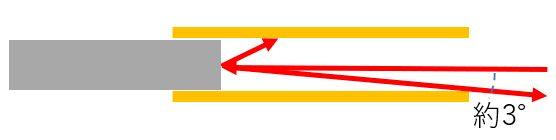
\includegraphics[width=50mm]{picture/setup/stoppermoshi2.png}\\
    \subcaption{ビームストッパー内で反射した場合}
    \label{stmoshi2}
  \end{minipage}
  \caption{ビームストッパーの模式図\cite{2019}}
\end{figure}


\end{document}
\documentclass[a4paper,11pt,dvipdfmx]{jsarticle}

\usepackage{bm}
\usepackage[dvipdfmx]{graphicx}
\usepackage[subrefformat=parens]{subcaption}
\usepackage[dvipdfmx]{color}
\usepackage{ascmac}
\usepackage{siunitx}
\usepackage{otf}
\pagestyle{plain}
\usepackage{float}
\usepackage[dvipdfmx]{hyperref}
\usepackage{pxjahyper}
\usepackage{here}
\usepackage{titlesec}
\titleformat*{\section}{\LARGE\bfseries}
\titleformat*{\subsection}{\normalsize\bfseries}
\usepackage{url}
\usepackage{comment}
\usepackage[table,xcdraw]{xcolor}
\hypersetup{% hyperrefオプションリスト
setpagesize=false,
 bookmarksnumbered=true,%
 bookmarksopen=true,%
 colorlinks=true,%
 linkcolor=blue,
 citecolor=blue,
}

\begin{document}


\subsection{検出過程}
散乱した粒子はPINフォトダイオードに入射しエネルギーを落として電流に変換される。本研究ではPINフォトダイオードからの電流がチャージアンプ・オペアンプに入り、シェーパーに入ることによって散乱粒子・反跳粒子を検出した。本研究ではADCとMCAを利用して波高を読むためチャージアンプ出力をシェーピングする必要があった。そのためシェーパーを利用した。利用したシェーパーは豊伸電子製N012である。

\subsubsection{PINフォトダイオード}
一般的にフォトダイオードというのは、半導体のPN接合部に光を照射すると電流や電圧を発生する受光素子である。検出から電気信号への変換効率が良いため、エネルギー分解能が良いという利点がある。PINフォトダイオードは、PN接合部の間にI型半導体を挟んだ検出器である。外部からの逆バイアス電圧が必要だが、空乏層が広くなるため、陽子のエネルギーを確実に落とし切れるという利点がある。\cite{pin}

 \begin{figure}[H]
    \centering
    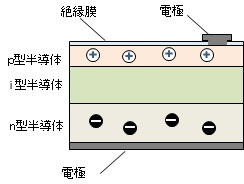
\includegraphics[width=50mm]{picture/setup/pinmoshi.png}
    \caption{PINフォトダイオードの模式図\cite{pin}}
    \label{pin1}
  \end{figure}

逆バイアス電圧がかけられたPINフォトダイオードに、陽子が入射すると、そのエネルギーによってI型半導体内で電離が発生する。I型半導体に電圧をかけることによってできた電界によって図\ref{pin2}のように電子とホールが移動し、電流が流れる仕組みとなっている。この電荷量の測定を行い入射粒子のエネルギーを推定できる。I型半導体の部分がSiの場合、電離する電子-ホール対を1組作成するには300Kで3.62eV必要なため、3MeV程度の散乱陽子ならば、およそ10$^\text{6}$組の対を生成することになる。よって、測定される電荷量が素電荷の値に生成される電子-ホール対の数をかけて、およそ0.16pCになる\cite{2019}。

\par
本実験で用いたPINフォトダイオードは、浜松ホトニクス製のS3590-09である。

 \begin{figure}[H]
    \centering
    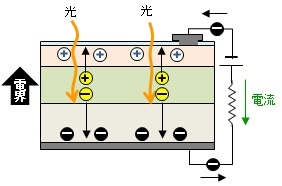
\includegraphics[width=50mm]{picture/setup/pinmoshi2.png}
    \caption{PINフォトダイオードによるエネルギー測定\cite{pin}}
    \label{pin2}
  \end{figure}

\subsubsection{チャージアンプ・オペアンプ}
PINフォトダイオードから流れた電荷信号は、オペアンプによって増幅され、チャージアンプによって電圧信号に変換される。チャージアンプの回路図を図\ref{kairo}に、チャージアンプの写真を図\ref{tya-jianpu}に示す。オペアンプはチャージアンプ回路に含まれており、クリアパルス製CS-515を利用している。本実験では、散乱粒子と反跳粒子の両方を観測したいため、先行研究\cite{2019}で利用していたチャージアンプ回路をもう1つ作成した。また、チャージアンプ回路単体では真空チェンバー内に置くことが不可能であるため、先行研究で利用していたPINフォトダイオード固定台をもう1つ作成し、利用した。PINフォト固定台の写真を図\ref{koteidai}に示す。

 \begin{figure}[H]
    \centering
    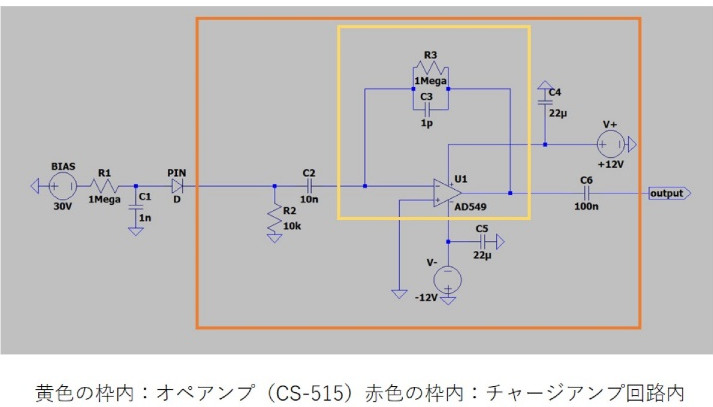
\includegraphics[width=80mm]{picture/setup/kairo.png}
    \caption{チャージアンプ回路図}
    \label{kairo}
  \end{figure}
  
  \begin{figure}[H]
   \begin{minipage}{0.32\linewidth}
    \centering
    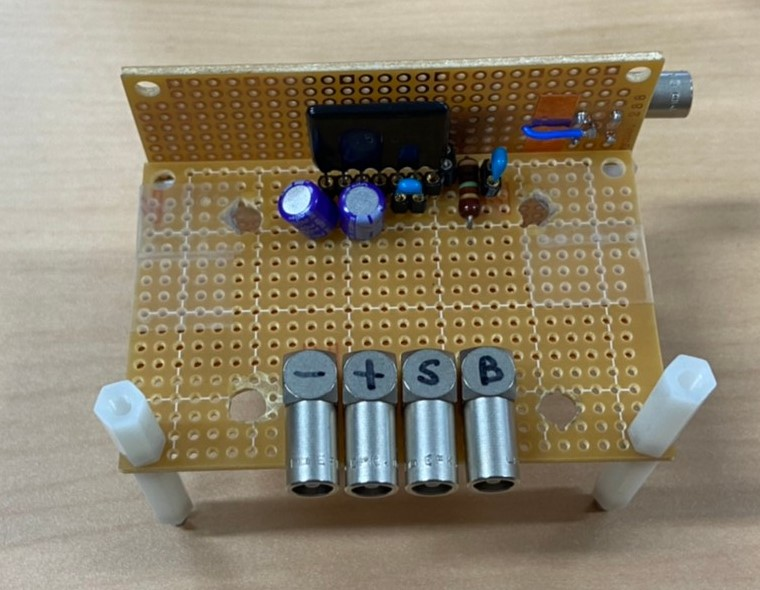
\includegraphics[width=30mm]{picture/setup/omote.jpg}
    \label{omote}
   \end{minipage}
   \begin{minipage}{0.32\linewidth}
    \centering
    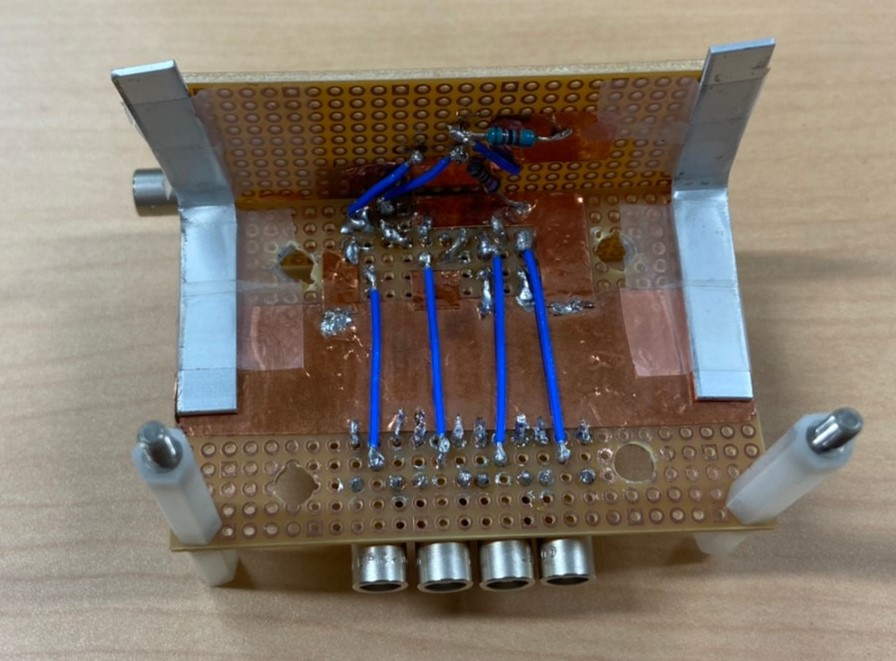
\includegraphics[width=30mm]{picture/setup/ura.jpg}
    \label{ura}
   \end{minipage}
   \begin{minipage}{0.32\linewidth}
    \centering
    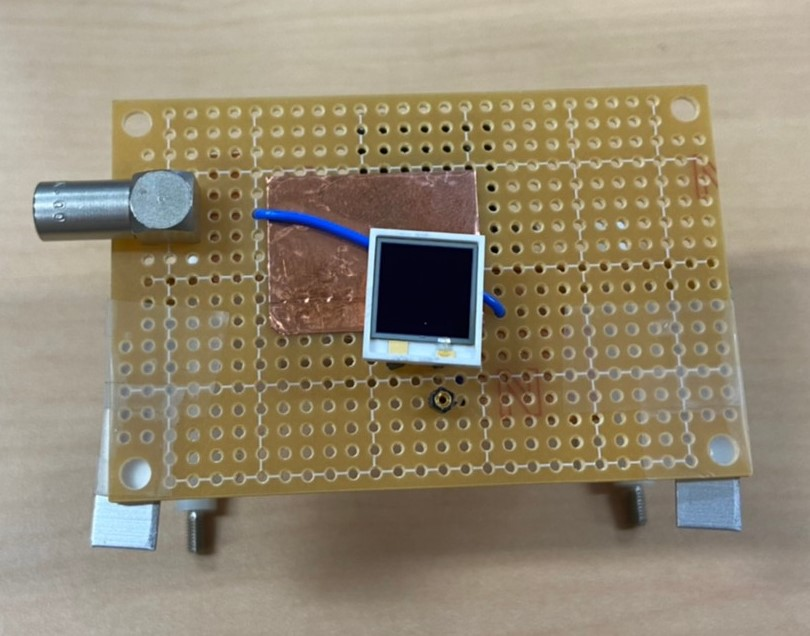
\includegraphics[width=30mm]{picture/setup/sokumen.jpg}
    \label{sokumen}
   \end{minipage}
  \caption{チャージアンプの写真}
  \label{tya-jianpu}
\end{figure}

 \begin{figure}[H]
    \centering
    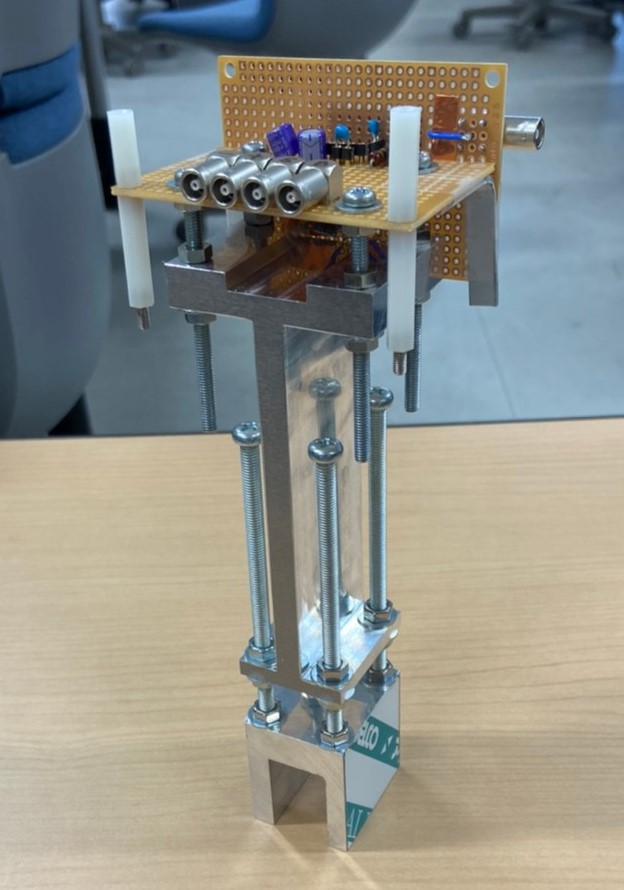
\includegraphics[width=40mm]{picture/setup/koteidai.jpg}
    \caption{PINフォト固定台の写真}
    \label{koteidai}
  \end{figure}
  
\end{document}
\documentclass[a4paper,11pt,dvipdfmx]{jsarticle}

\usepackage{bm}
\usepackage[dvipdfmx]{graphicx}
\usepackage[subrefformat=parens]{subcaption}
\usepackage[dvipdfmx]{color}
\usepackage{ascmac}
\usepackage{siunitx}
\usepackage{otf}
\pagestyle{plain}
\usepackage{float}
\usepackage[dvipdfmx]{hyperref}
\usepackage{pxjahyper}
\usepackage{here}
\usepackage{titlesec}
\titleformat*{\section}{\LARGE\bfseries}
\titleformat*{\subsection}{\normalsize\bfseries}
\usepackage{url}
\usepackage{comment}
\usepackage[table,xcdraw]{xcolor}
\hypersetup{% hyperrefオプションリスト
setpagesize=false,
 bookmarksnumbered=true,%
 bookmarksopen=true,%
 colorlinks=true,%
 linkcolor=blue,
 citecolor=blue,
}

\begin{document}


\subsection{ターゲット}
1.6節より陽子ビームを当てるターゲットにポリエチレンと金を利用する。ポリエチレンにはコープキッチン用ポリ袋を、金にはカタニ産業の金箔24Kを利用する。

\subsubsection{ターゲットの厚さ}
各社の出すターゲットの厚さの精度が低いため、ポリエチレンはµメーターで計測し、金は密度と体積が分かった状態で質量を計測し厚さを求めた。それぞれの表記値と計測値を表\ref{thickness}に示す。

\begin{table}[H]
 \centering
 \begin{tabular}{cccll}
 \cline{1-3}
  \multicolumn{1}{|c|}{}       & \multicolumn{1}{c|}{表記値}    & \multicolumn{1}{c|}{計測値}           &  &  \\ \cline{1-3}
  \multicolumn{1}{|c|}{ポリエチレン} & \multicolumn{1}{c|}{10µm}   & \multicolumn{1}{c|}{11.5±0.2µm}    &  &  \\ \cline{1-3}
  \multicolumn{1}{|c|}{金}      & \multicolumn{1}{c|}{約0.1µm} & \multicolumn{1}{c|}{0.161±0.006µm} &  &  \\ \cline{1-3}
  \multicolumn{1}{l}{}         & \multicolumn{1}{l}{}        & \multicolumn{1}{l}{}               &  & 
 \end{tabular}
 \caption{ターゲットの厚さの表記値と計測値}
 \label{thickness}
\end{table}

\subsubsection{ターゲットホルダー}
ポリエチレンはセロハンテープでアルミ板に張り付け、ターゲットに水平方向から検出器の角度が小さい場合にも測定できるように固定した。金に関しては非常に薄くセロハンテープ等で固定することは不可能であるため、先行研究と同様に2枚のアルミ板でターゲットを挟み、ネジで固定した。このターゲットホルダーはターゲットが露出す津中心部が削られているため、なるべく大きな散乱角に対応することが可能である。図\ref{poli}にポリエチレンのターゲットを、図\ref{gold}に金のターゲットを、図\ref{goldtokutyou}に金のターゲットホルダーの特徴を示す。
\par
ターゲットをポリエチレンにして強いビームを一定時間当てると焦げが出来る、この焦げに合わせてターゲットとビームストッパーの位置調整を行った。焦げが出来たポリエチレンのターゲットを図\ref{koge}に示す。

  \begin{figure}[H]
    \centering
    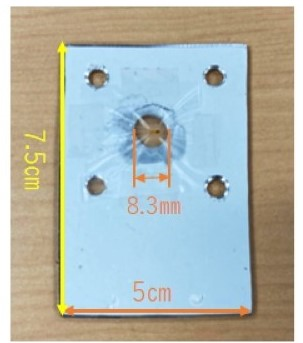
\includegraphics[width=35mm]{picture/setup/poli.jpg}
    \caption{ポリエチレンのターゲット}
    \label{poli}
  \end{figure}
  
  \begin{figure}[H]
    \begin{minipage}{0.5\hsize}
     \begin{center}
      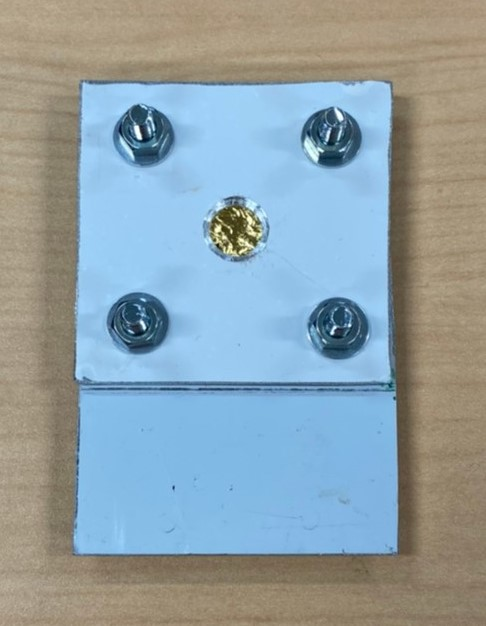
\includegraphics[width=30mm]{picture/setup/gold.jpg}
     \end{center}
     \caption{金のターゲット}
     \label{gold}
    \end{minipage}
    \begin{minipage}{0.5\hsize}
     \begin{center}
      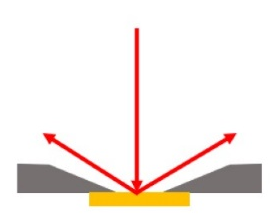
\includegraphics[width=40mm]{picture/setup/goldtokutyou.png}
     \end{center}
     \caption{金のターゲットホルダーの特徴}
     \label{goldtokutyou}
    \end{minipage}
  \end{figure}
  
  \begin{figure}[H]
    \centering
    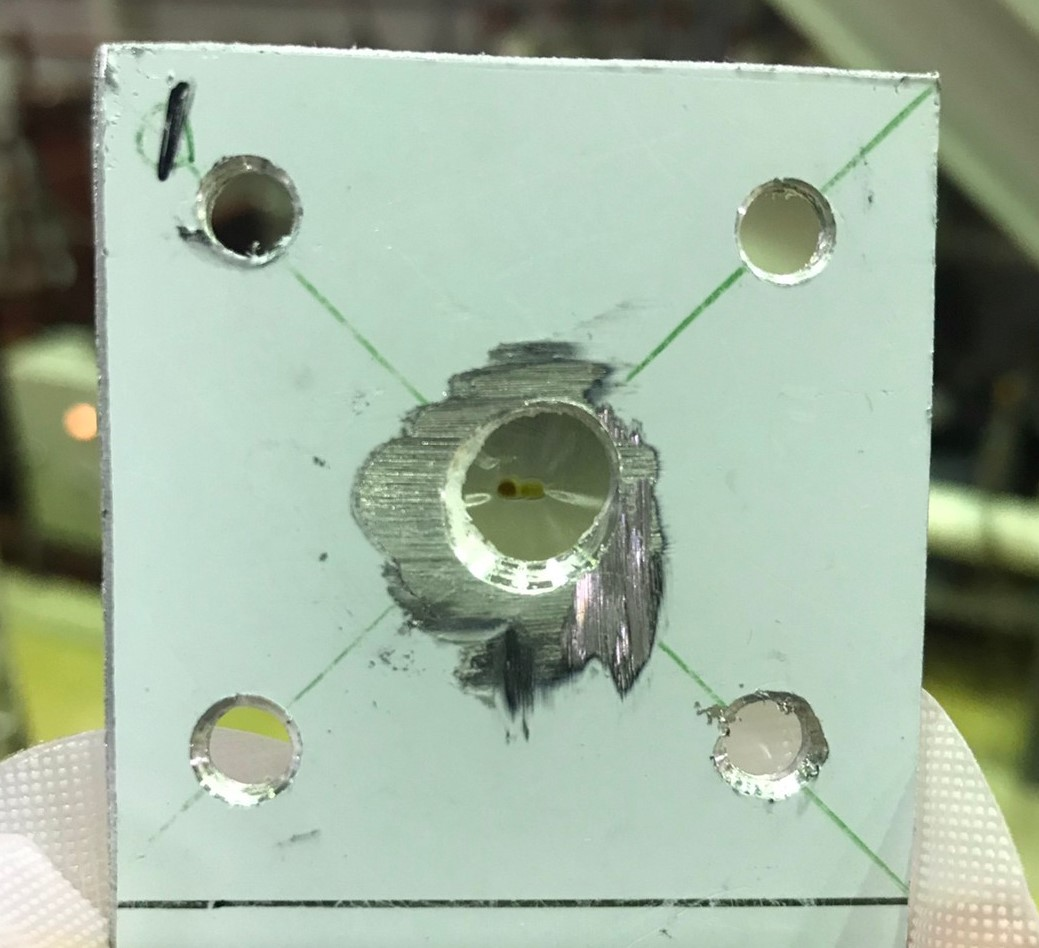
\includegraphics[width=35mm]{picture/setup/koge.jpg}
    \caption{焦げができたポリエチレンのターゲット}
    \label{koge}
  \end{figure}

\subsection{まとめ}
精度の良いピークを得るために、ビームストッパーを設置しバックグラウンドを防ぐこと、ターゲット(ポリエチレン)を直接アルミ板に貼り付け、ターゲットに水平方向から検出器の角度が小さい場合も測定できるようにしたこと。ポリエチレンにできたビームによるこげからビームストッパーの位置を決定することをした。また、散乱粒子と反跳粒子の両方を観測するため、検出回路をもう1台制作した。さらにターゲットの厚さを自ら計測することで精度の良い実験を行う工夫をした。

\end{document}
\documentclass[a4paper,11pt,dvipdfmx]{jsarticle}

\usepackage{bm}
\usepackage[dvipdfmx]{graphicx}
\usepackage[dvipdfmx]{color}
\usepackage[subrefformat=parens]{subcaption}
\usepackage{ascmac}
\usepackage{siunitx}
\usepackage{otf}
\pagestyle{plain}
\usepackage{float}
\usepackage[dvipdfmx]{hyperref}
\usepackage{pxjahyper}
\usepackage{here}
\usepackage{titlesec}
\titleformat*{\section}{\LARGE\bfseries}
\titleformat*{\subsection}{\normalsize\bfseries}
\usepackage{url}
\usepackage[table,xcdraw]{xcolor}
\hypersetup{% hyperrefオプションリスト
setpagesize=false,
 bookmarksnumbered=true,%
 bookmarksopen=true,%
 colorlinks=true,%
 linkcolor=blue,
 citecolor=blue,
}


\begin{document}
\newpage
\section{\LARGE{データ収集と解析(担当:金\UTF{FA11})}}

\subsection{DAQ systemの構築}
本節ではDAQ system(Data AcQuition system:データ収集系)について述べる。本研究ではターゲット原子核へ陽子を入射し、散乱後の粒子のエネルギースペクトルを得ることで、散乱断面積を求める。検出器であるPINフォトダイオードの出力信号の波高から、スペクトルを得るためのDAQ systemの構築を目指した。
\subsubsection{手段の検討}
昨年度のラザフォード散乱実験\cite{2019}では波高データの読み出しにはMCA(Multi Channel Analyzer)を使用していた。以下にその検出回路を示す。

\vspace*{5mm}

\begin{figure}[H]
\centering
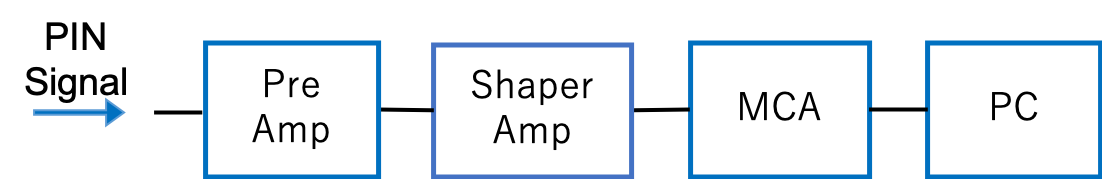
\includegraphics[width=100mm]{picture/daq/MCA.png}
%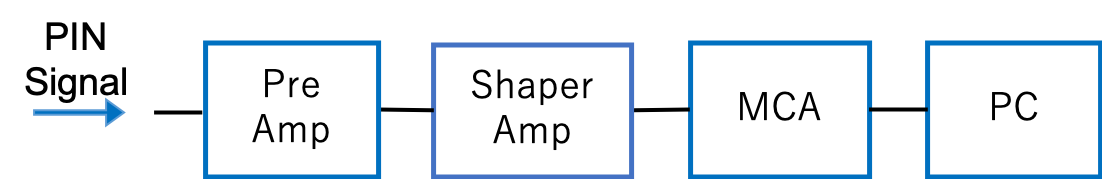
\includegraphics[bb=0 0 1102 179,width=100mm]{picture/daq/MCA.png}
\caption{MCAを用いた検出回路}
\label{MCA}
\end{figure}

\vspace*{5mm}

本年度の新たな試みとして、p-p散乱の観測を目指したことが挙げられる。昨年度使用していたMCAでは、同じ散乱イベント由来の波高データを時間同期しながら得ることができなかった。そこでVME busモジュールを用いた2ch同時計測回路の構築を行うこととした。

\subsubsection{VME bus}
VME bus(Versa Module Eurocard bus)とは1981年に開発されたコンピュータのバス規格の一つである。同じく高エネルギー物理学実験などに用いられるCAMAC 規格と比べてデータ転送が速いという特徴を持つ。VMEクレートに挿入されたモジュールはバックブレーンを介してデータの通信を行う。本研究ではピークホールド型のADCと、SiTCP VME Masterの2つのモジュールを用いた。以下その役割や性能を述べる。

\newpage
\begin{description}
   \item[● ピークホールド型ADC]\mbox{}\\
   ADC(Analog-to-Digital Converter)とはアナログ信号をデジタル値に変換するシステムである。信号の波高分布を得るため、本研究ではピークホールド型のADC(以降PHADC)を用いた。PHADCのGate入力端子に信号が与えられている間のピーク電圧をデジタル変換する。\\

   \item[● SiTCP VME Master]\mbox{}\\
   Eathernet経由でVME busを制御するためのMaster Moduleである。同一のクレートに挿入されている VME Slave Moduleへのアクセスが可能。PHADCの制御・データ読み出しに用いた。
   
\vspace*{5mm}
   
 \begin{figure}[H]
    \begin{tabular}{cc}
      \begin{minipage}[t]{0.45\hsize}
        \centering
        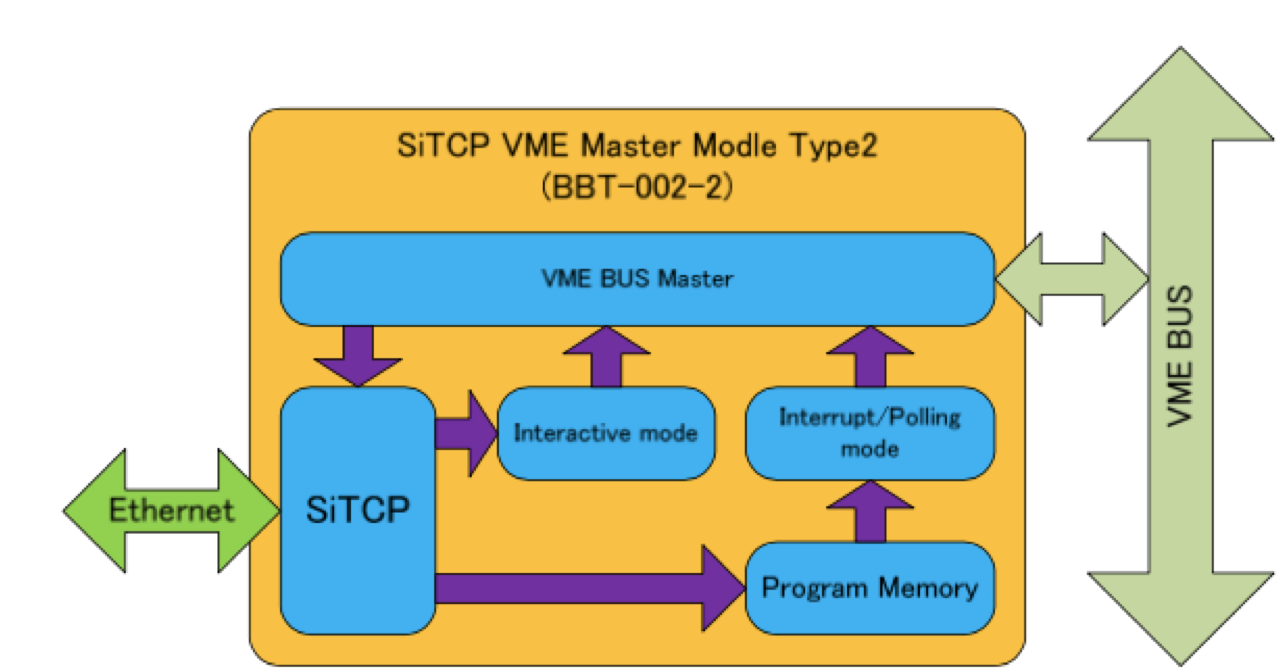
\includegraphics[width=62mm,height=50mm]{picture/daq/SiTCP.png}
        \caption{SiTCP 全体ブロック図\cite{BBT}}
        \label{SiTCP1}
      \end{minipage} &
      \begin{minipage}[t]{0.45\hsize}
        \centering
        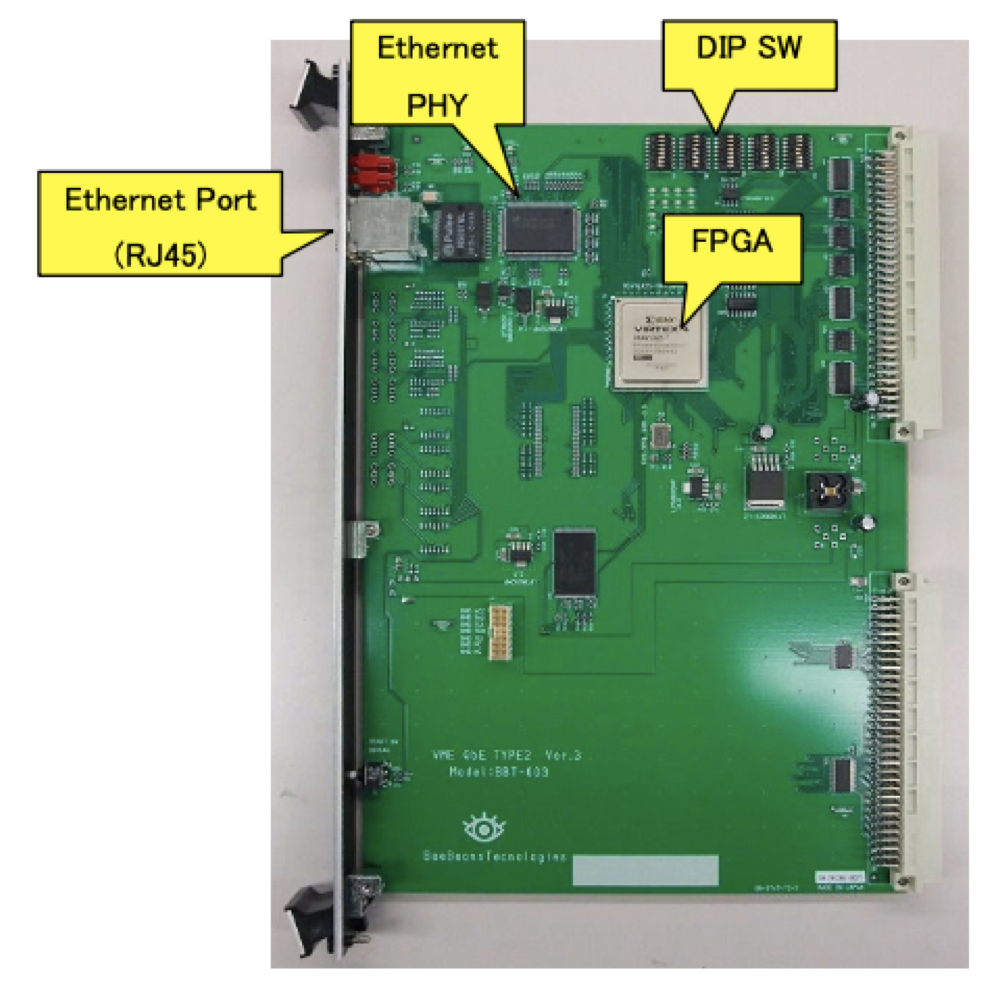
\includegraphics[width=64mm,height=70mm]{picture/daq/SiTCP2.png}
        \caption{SiTCP 全体写真\cite{BBT}}
        \label{SiTCP2}
      \end{minipage}
    \end{tabular}
  \end{figure}
  
\end{description}

\vspace*{5mm}

\begin{table}[h]
   \caption{使用したVMEモジュール\cite{BBT}\cite{hoshin}}
   \centering
   
  \begin{tabular}{ccc} \hline
  モジュール名 & 制作元:型番 & スペック等 \\ \hline \hline
  PHADC & 豊伸電子:8ch PHADC V006 & 
  \begin{tabular}{c}
    最大入力:4V\\
    逐次14bit変換\\
    入力インピーダンス:1k$\Omega$ \\
    最小Gate幅:500ns
   \end{tabular} \\ \hline
    SiTCP VME Master & BeeBeansTechnologies:BBT-002-2 &
    \begin{tabular}{c}
    通信プロトコル:TCP
   \end{tabular} \\ \hline

  \end{tabular}
  \centering
\end{table}

\newpage
\subsubsection{2ch同時計測回路の構築}
前節で述べたように、PHADCにはTrigger信号としてGate入力を与える必要がある。入射陽子と反跳水素原子核は、散乱イベント発生からおよそ同じ時間で検出器に到達すると予想される。(散乱後の二粒子のエネルギー差を考慮した理論的な到達時間の最大差 < 10ns )。したがって2つの信号を同時計数回路(コインシデンス)へ入力すれば、適切なタイミングでTriggerをかけることができると考えた。以下に2ch同時計測回路のブロック図[図\ref{coin}]と使用したNIMモジュール[表\ref{NIM}]を示す。ルーターにはbuffalo社のWSR-1800AX4-BKを用いた。

\vspace*{7mm}

\begin{figure}[H]
\centering
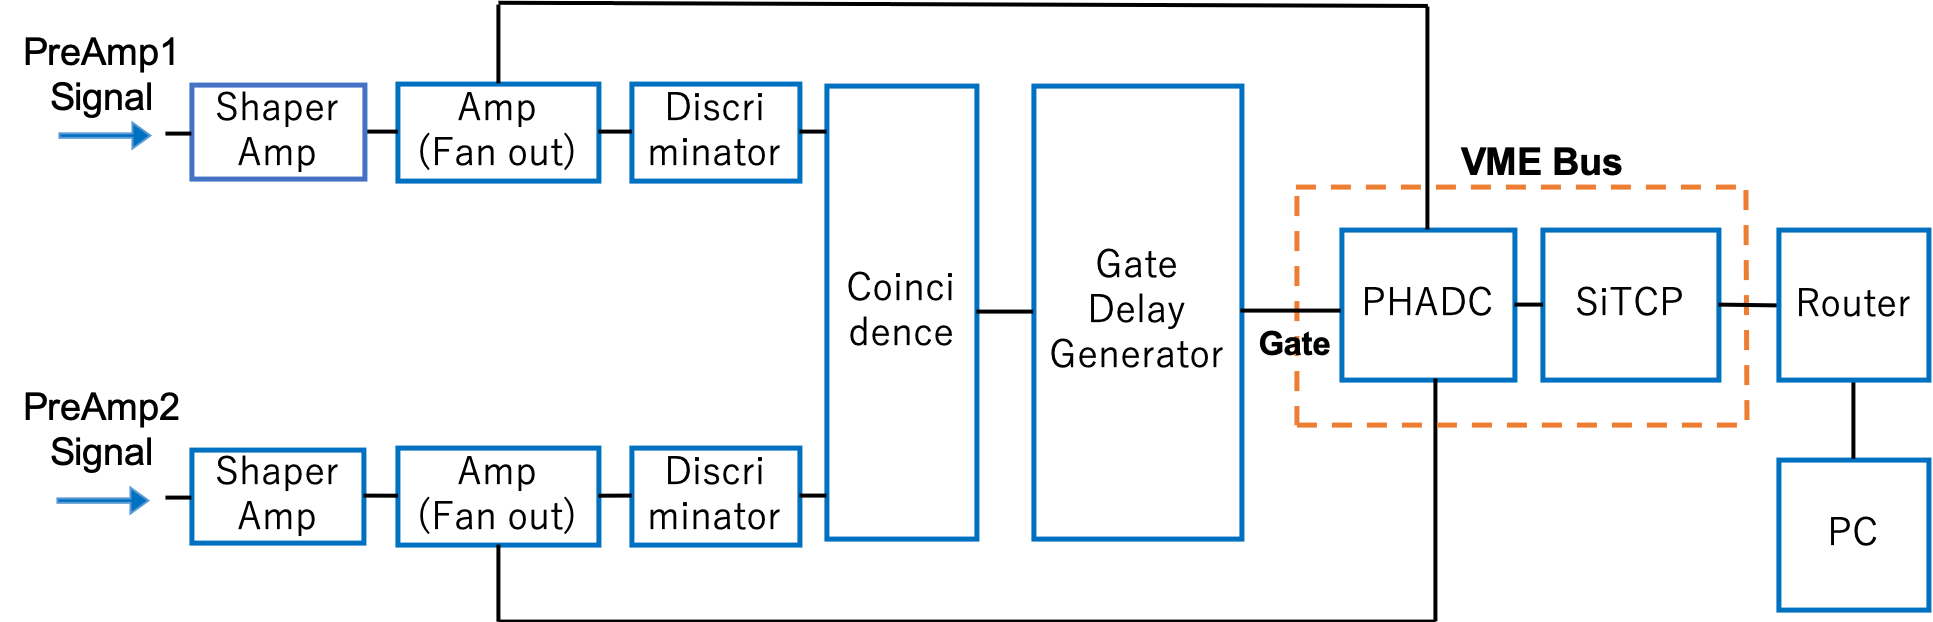
\includegraphics[width=150mm,height=60mm]{picture/daq/PHADC.png}
\caption{2ch同時計測回路}
\label{coin}
\end{figure}

\vspace*{5mm}

\begin{table}[h]
   \caption{使用したNIMモジュール\cite{hoshin}\cite{repic}}
   \centering
   
\begin{tabular}{ccc} \hline
  モジュール名 & 制作元:型番 & スペック、実験時の設定等 \\ \hline \hline
  アンプ & 豊伸電子:N018 & 出力gain:10 \\ \hline
  コインシデンス & 豊伸電子:N017 & 
  \begin{tabular}{c}
    応答速度:2ns~ \\
    アナログ加算式(ANY1$\sim$4)
   \end{tabular} \\ \hline
    ゲートジェネレーター & 豊伸電子:N014 & Gate幅:約1$\mu$s \\ \hline
    ディスクリミネーター & ハヤシレピック:RPN-110 & 最小Threshold:-20mV \\ \hline
    シェーパーアンプ & 豊伸電子:N012 &
    \begin{tabular}{c}
    時定数:0.15$\mu$s \\
    出力gain:ADC$\rightarrow$10、MCA$\rightarrow$20
    \end{tabular} \\ \hline
  \label{NIM}
  \end{tabular}
  \centering
\end{table}

\newpage
\subsubsection{Trigger Logic}\label{logic}
ここではTriggerシステムについて述べる。まずは使用したモジュールの説明を行う。\\
\begin{description}
   \item[● ディスクリミネーター(波高弁別回路)]\mbox{}\\
   Threshold電圧より大きい入力信号が与えられたとき、矩形波を出力する\\
   \item[● コインシデンス(同時計数回路)]\mbox{}\\
   4つの入力チャンネルを持つ。本論文では4つのうちいずれか1つ以上に信号が入力されたときに矩形波を出力するモードがANY1、2つ以上に入力があったときに矩形波を出力するモードをANY2と定義する。\\
   \item[● ゲートディレイジェネレーター]\mbox{}\\
   信号入力があったとき、任意の時間幅の矩形波を出力する。出力時間にディレイをかけることもできるが、本実験ではディレイ機能は用いていない。\\
\end{description}

\noindent
本実験で用いたTriggerシステムの概略を図\ref{Logic}に示す。
ディスクリミネーターにはプリアンプ・シェイパーアンプ・アンプを通した信号を入力している。この入力に対してディスクリミネーターが矩形波を出力し、2チャンネルで同時に出力されたときにコインシデンスが矩形波を出力する。その信号をゲートジェネレーターに入力することで、TriggerとなるGate信号を作成した。

\vspace*{5mm}

\begin{figure}[H]
\centering
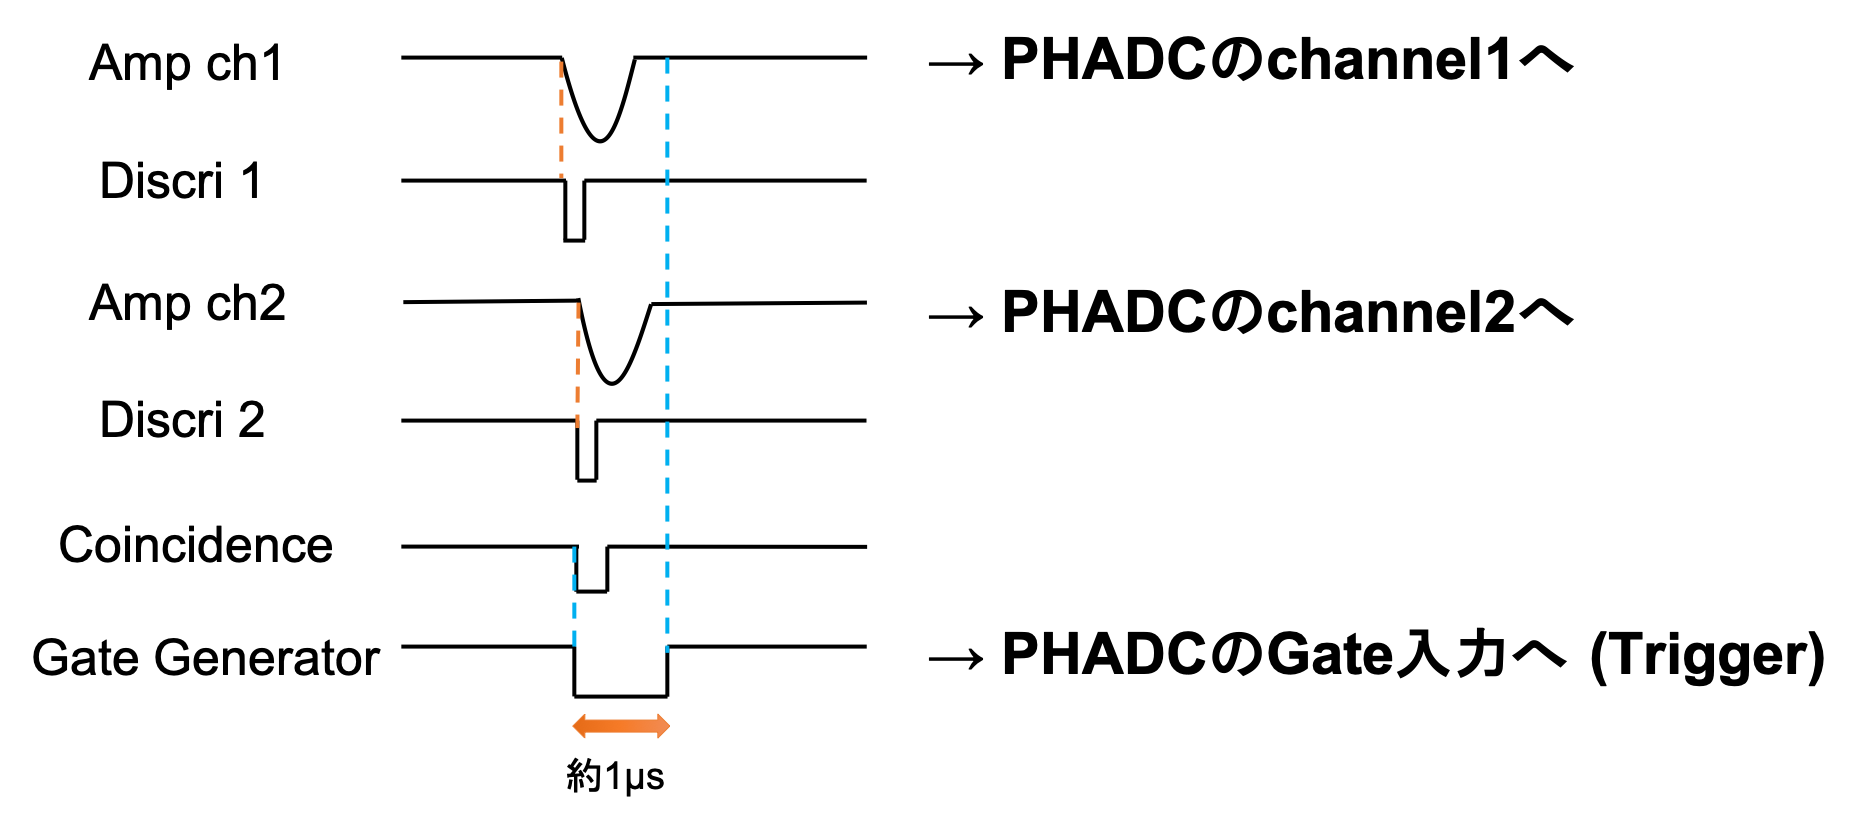
\includegraphics[width=150mm,height=65mm]{picture/daq/Trigger.png}
\caption{Trigger Logic}
\label{Logic}
\end{figure}

\newpage
\subsubsection{その他の設定}
ディスクリミネーターのThresholdは、真空チェンバー内でのノイズを拾わないレベルの電圧値で設定を行なった。パルスジェネレーターでその電圧値を確認したところ、およそ-100mVであった。

ゲートジェネレーターの出力の時間幅は、PINフォトダイオードに $\alpha$ 線($^{241}\mathrm{Am}$線源)を照射したときの信号を用いておよそ1$\mu$sに設定した。またPHADCは正負のどちらでもピーク電圧をデジタル変換するようになっているが、負の電圧に比べて正の電圧を入力した方がデータ収集が安定したため負の信号から正の信号へと変換を行なった。変換にはPulse Electronis社のPE-62245を用いた。[図\ref{Gate}]

\vspace*{5mm}

 \begin{figure}[H]
    \begin{tabular}{cc}
      \begin{minipage}[t]{0.50\hsize}
        \centering
        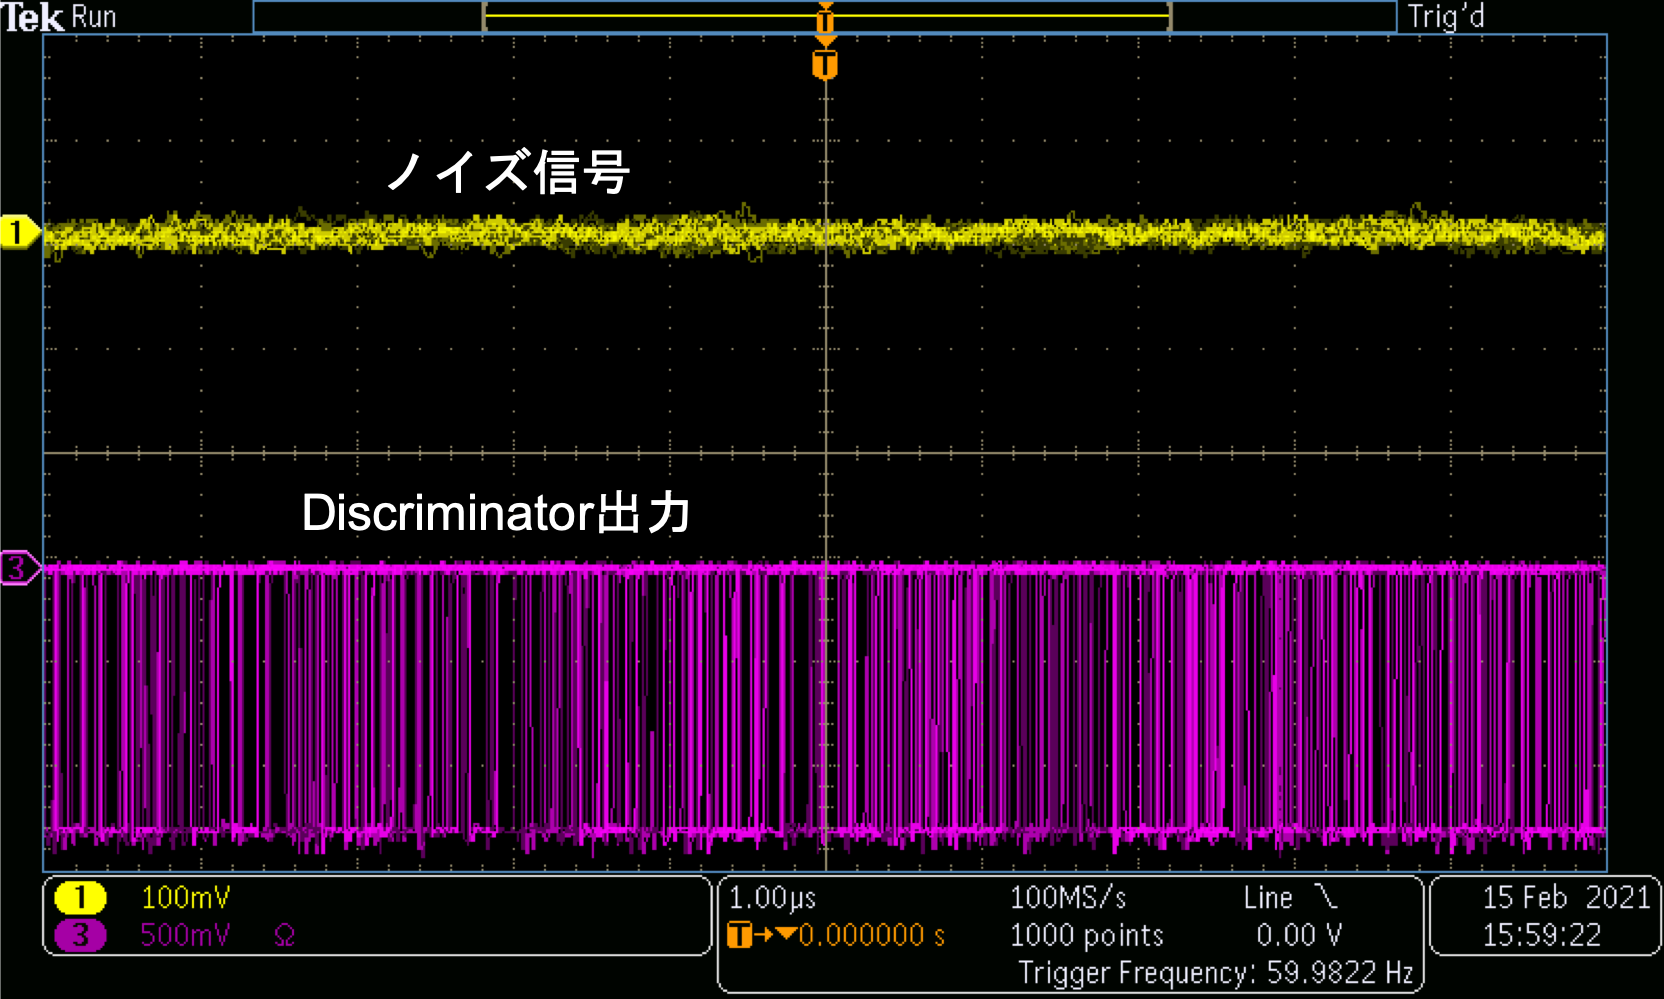
\includegraphics[width=65mm,height=42mm]{picture/daq/noise.png}
        \caption{ノイズ信号にディスクリミネーターが反応している様子}
        \label{noise}
      \end{minipage} &
      \begin{minipage}[t]{0.50\hsize}
        \centering
        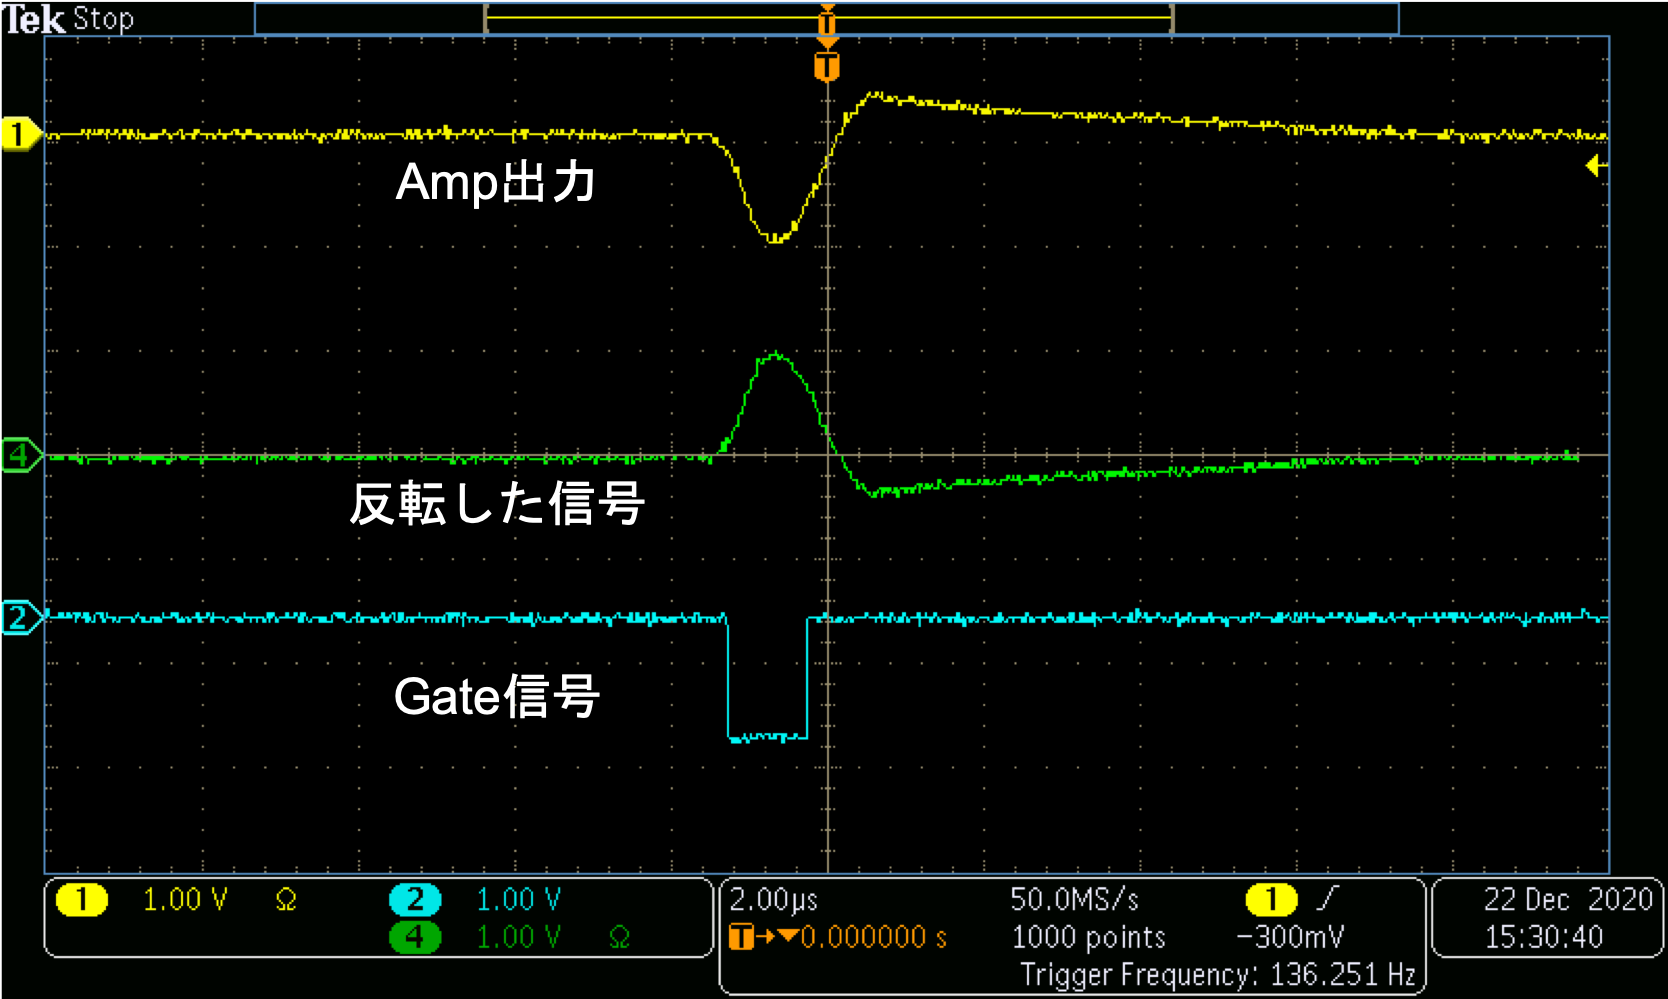
\includegraphics[width=65mm,height=42mm]{picture/daq/Gate.png}
        \caption{信号の反転とGate信号}
        \label{Gate}
      \end{minipage}
    \end{tabular}
  \end{figure}

\vspace*{3mm}

\begin{figure}[H]
\centering
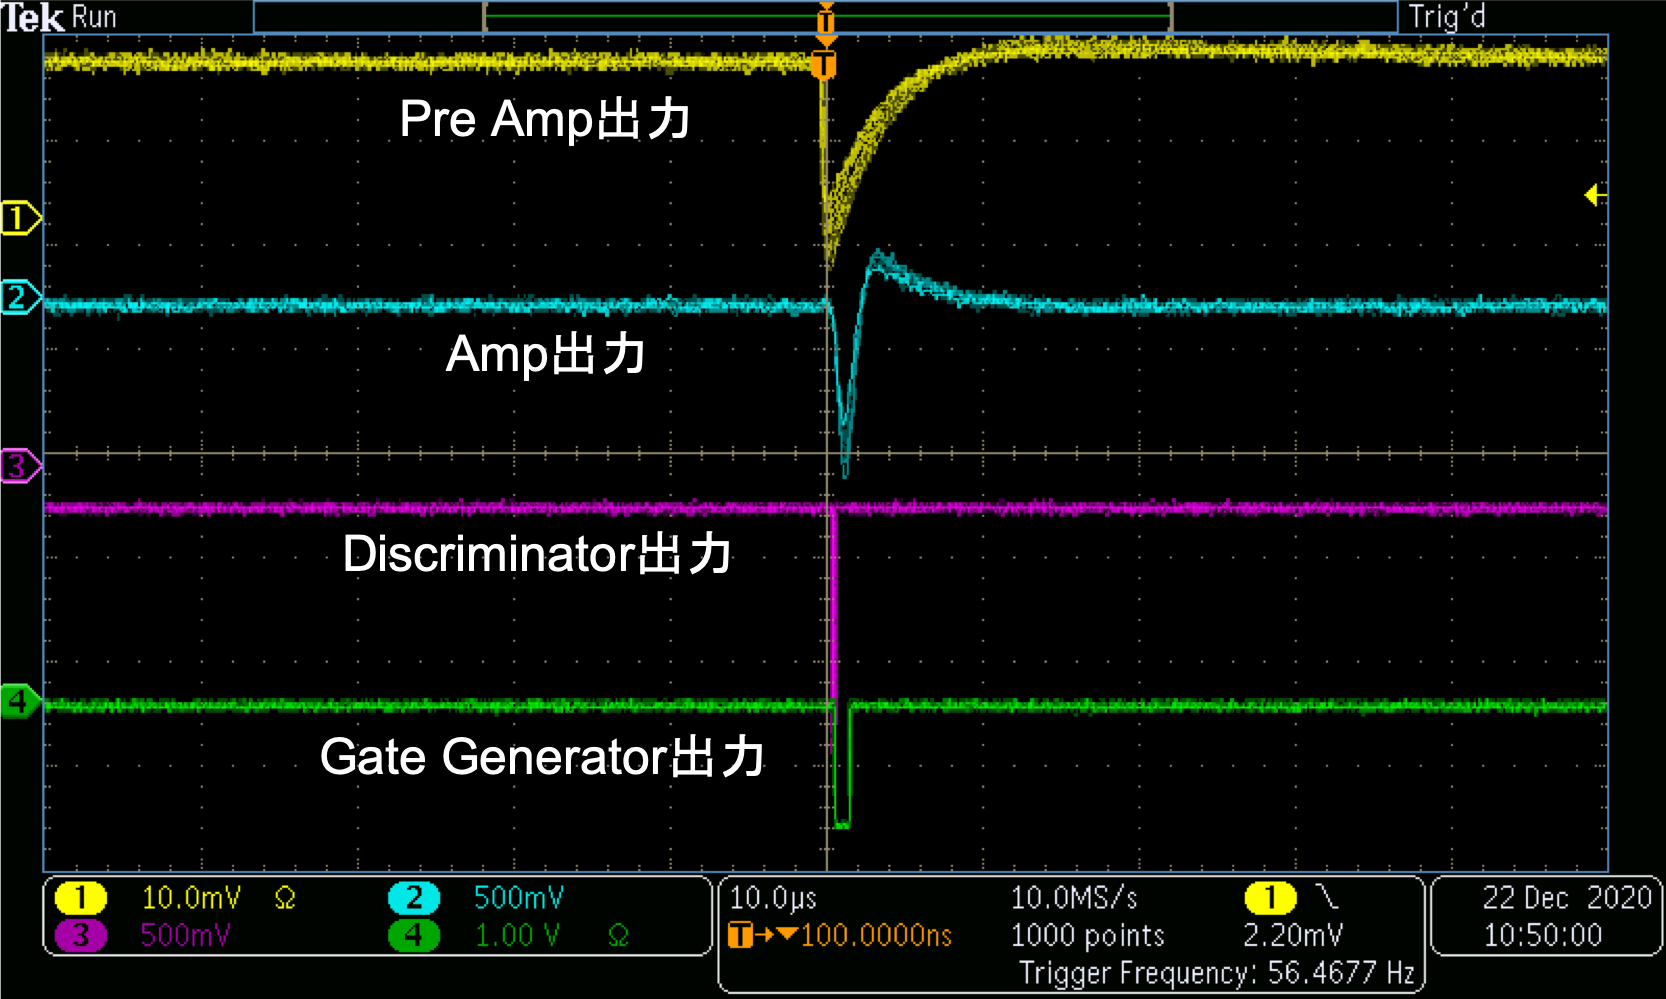
\includegraphics[width=100mm,height=60mm]{picture/daq/signal.png}
\caption{適切な各モジュールの出力}
\label{signal}
\end{figure}

\newpage
\subsection{DAQ systemの動作確認}
海事科学部での本実験の前に、DAQ systemの動作確認を行なった。確認事項としては、得られるエネルギースペクトルおよびその解析プログラム、2ch同時計測回路の動作、そしてトリガーレート等が挙げられる。本節ではその試験結果を述べる。

\subsubsection{エネルギースペクトル}
正しいエネルギースペクトルが得られているかは、PINフォトダイオードに$\alpha$ 線($^{241}\mathrm{Am}$線源)を照射することで確認した。$\alpha$線源とPINフォトダイオードとの距離を0$\sim$2cmの1cmごとに設定し、計測を行うことで空気中でのエネルギー損失の要素を含んだエネルギースペクトルが得られるかを試みた。$\alpha$線や陽子線などの重荷電粒子は物質中を透過するとき、進行方向の物質を励起しながらエネルギーを失っていく。図\ref{Bragg}に、5.49 MeVの$\alpha$線の空気中でのBragg曲線を示す。$^{241}\mathrm{Am}$線源における$\alpha$線のエネルギーは5.4 MeVであるが、エネルギー損失の過程は同様なBragg曲線 に従うと考えられる。図\ref{0to2}に得られたエネルギースペクトルを示す。距離が大きくなるにつれて、波高が小さくなっていく様子が見られる。この結果から正常に動作していると評価した。\\

%\vspace*{5mm}
\begin{figure}[H]
\centering
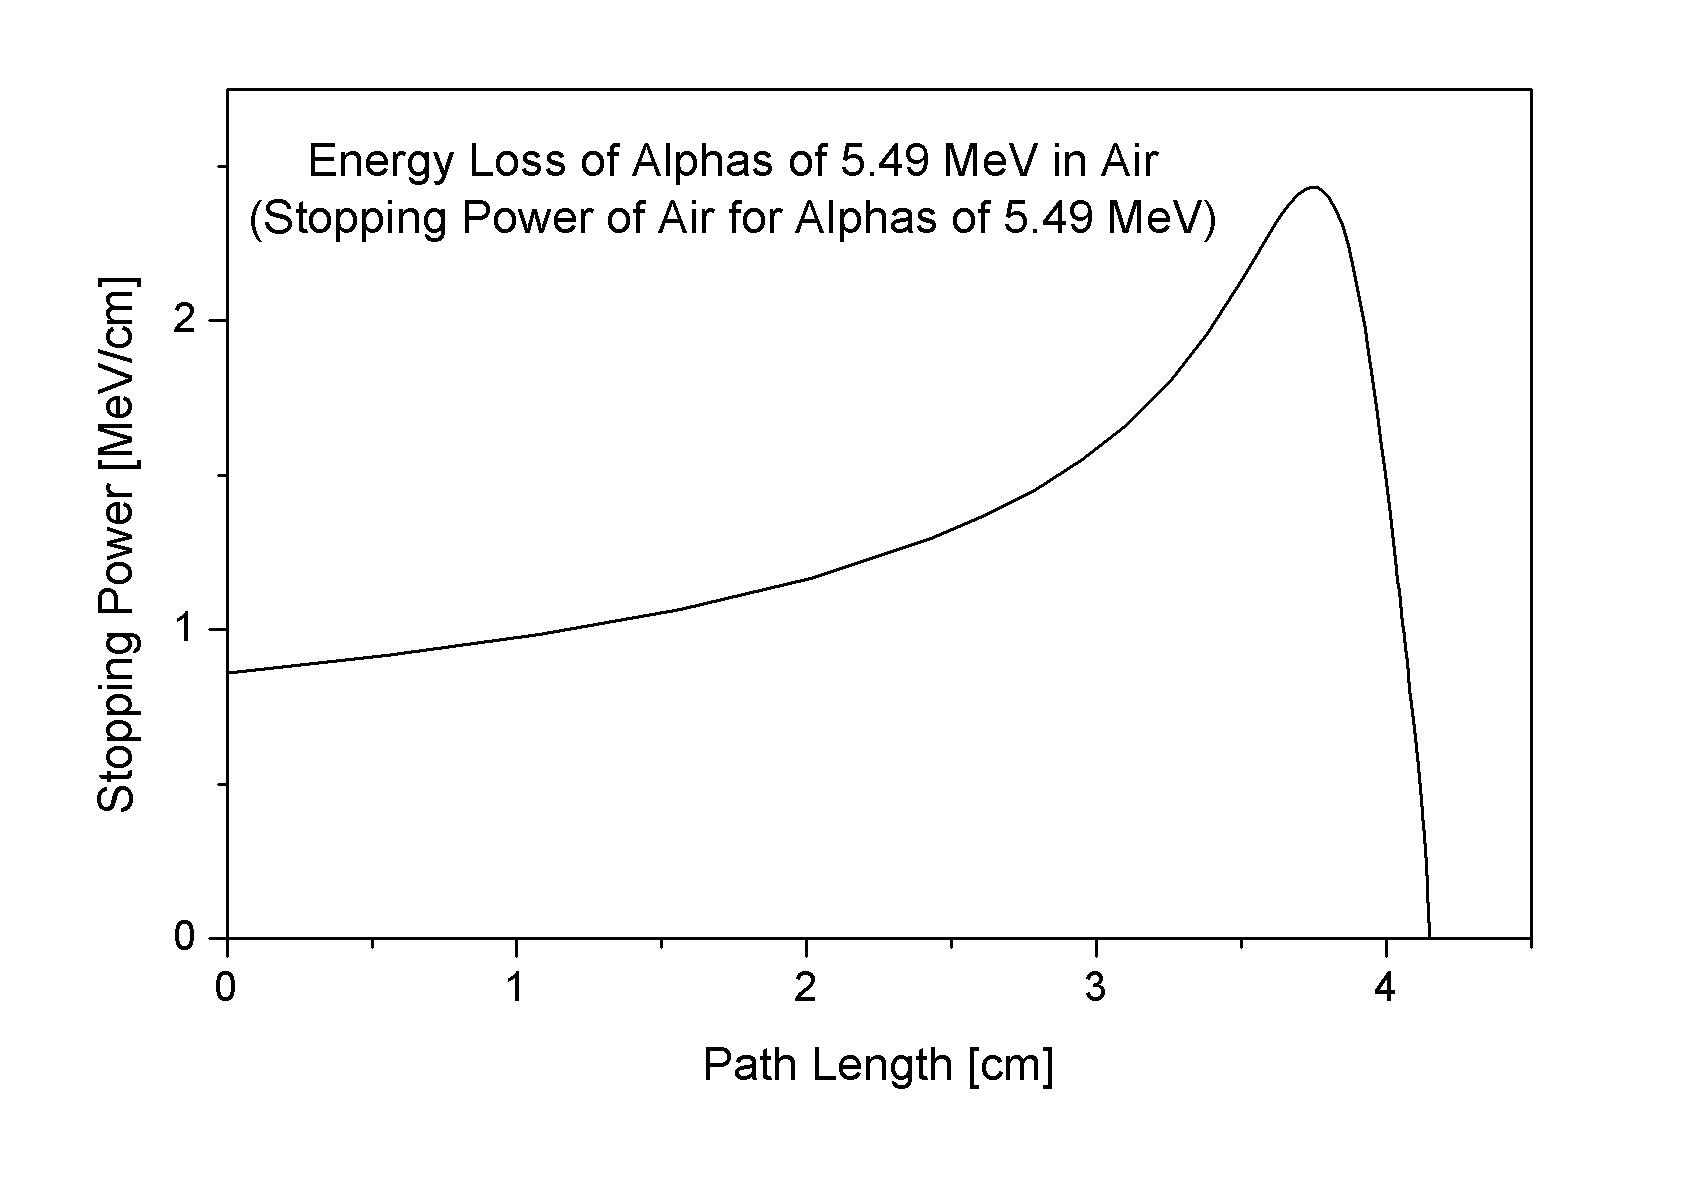
\includegraphics[width=120mm]{picture/daq/Bragg.png}
\caption{5.49 MeVの$\alpha$線に対するBragg曲線\cite{braggpeak}}
\label{Bragg}
\end{figure}

\begin{figure}[H]
\centering
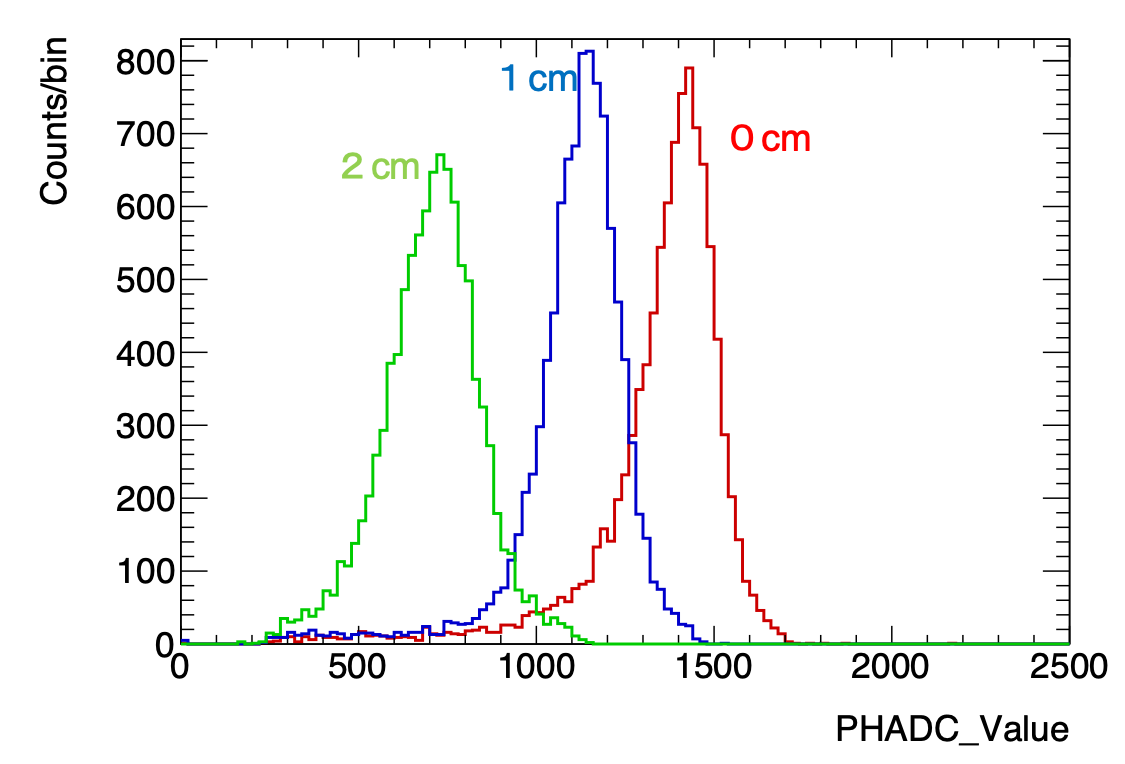
\includegraphics[width=110mm]{picture/daq/0to2cm.png}
\caption{3つの検出距離におけるエネルギースペクトル}
\label{0to2}
\end{figure}
\begin{figure}[H]
\centering
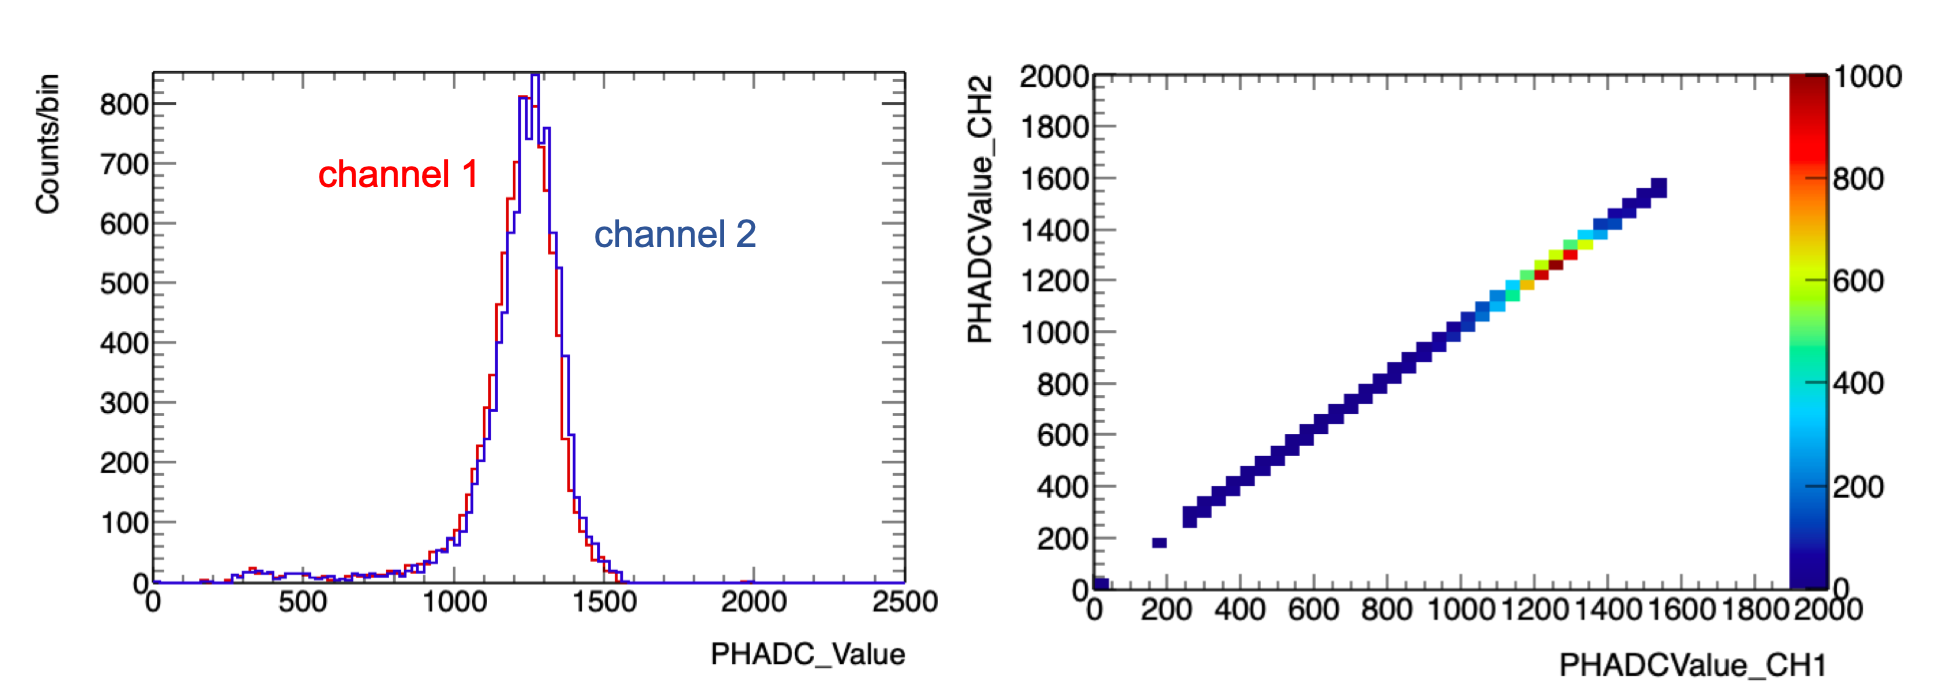
\includegraphics[width=155mm]{picture/daq/2ch.png}
\caption{2ch同時計測回路の試験結果}
\label{2ch}
\end{figure}

\subsubsection{2ch同時計測回路の確認}
2ch同時計測回路の動作確認は、$\alpha$線の信号を並列回路を用いて2つに増やしそれぞれPHADCに入力して行なった。2つのチャンネルで得られたエネルギースペクトルと二次元ヒストグラムを図\ref{2ch}に示す。

二次元ヒストグラムから、2つのチャンネルの値が等しくなっていることが分かる。この結果から2ch同時計測回路が正常に動作していると判断した。

\subsubsection{トリガーレートの考慮}
強い陽子ビームを照射すると、高いレートでトリガーがかかることが予想される。そこで事前にトリガーレートの上限値を検証する必要があった。PHADCのGate入力に、パルスジェネレーターを用いて指定したレートでパルスを入力し、1000イベント計測終了までの時間を記録し理論値との比較を行った。[図\ref{trigger}]

理論上では計測にかかる時間はパルスのレートと反比例の関係にあるが、図\ref{trigger}にあるように、1ch計測回路では90Hz、2ch同時計測回路では70Hzあたりを境に計測時間は理論の値よりも大きくなっている。

\begin{figure}[H]
\centering
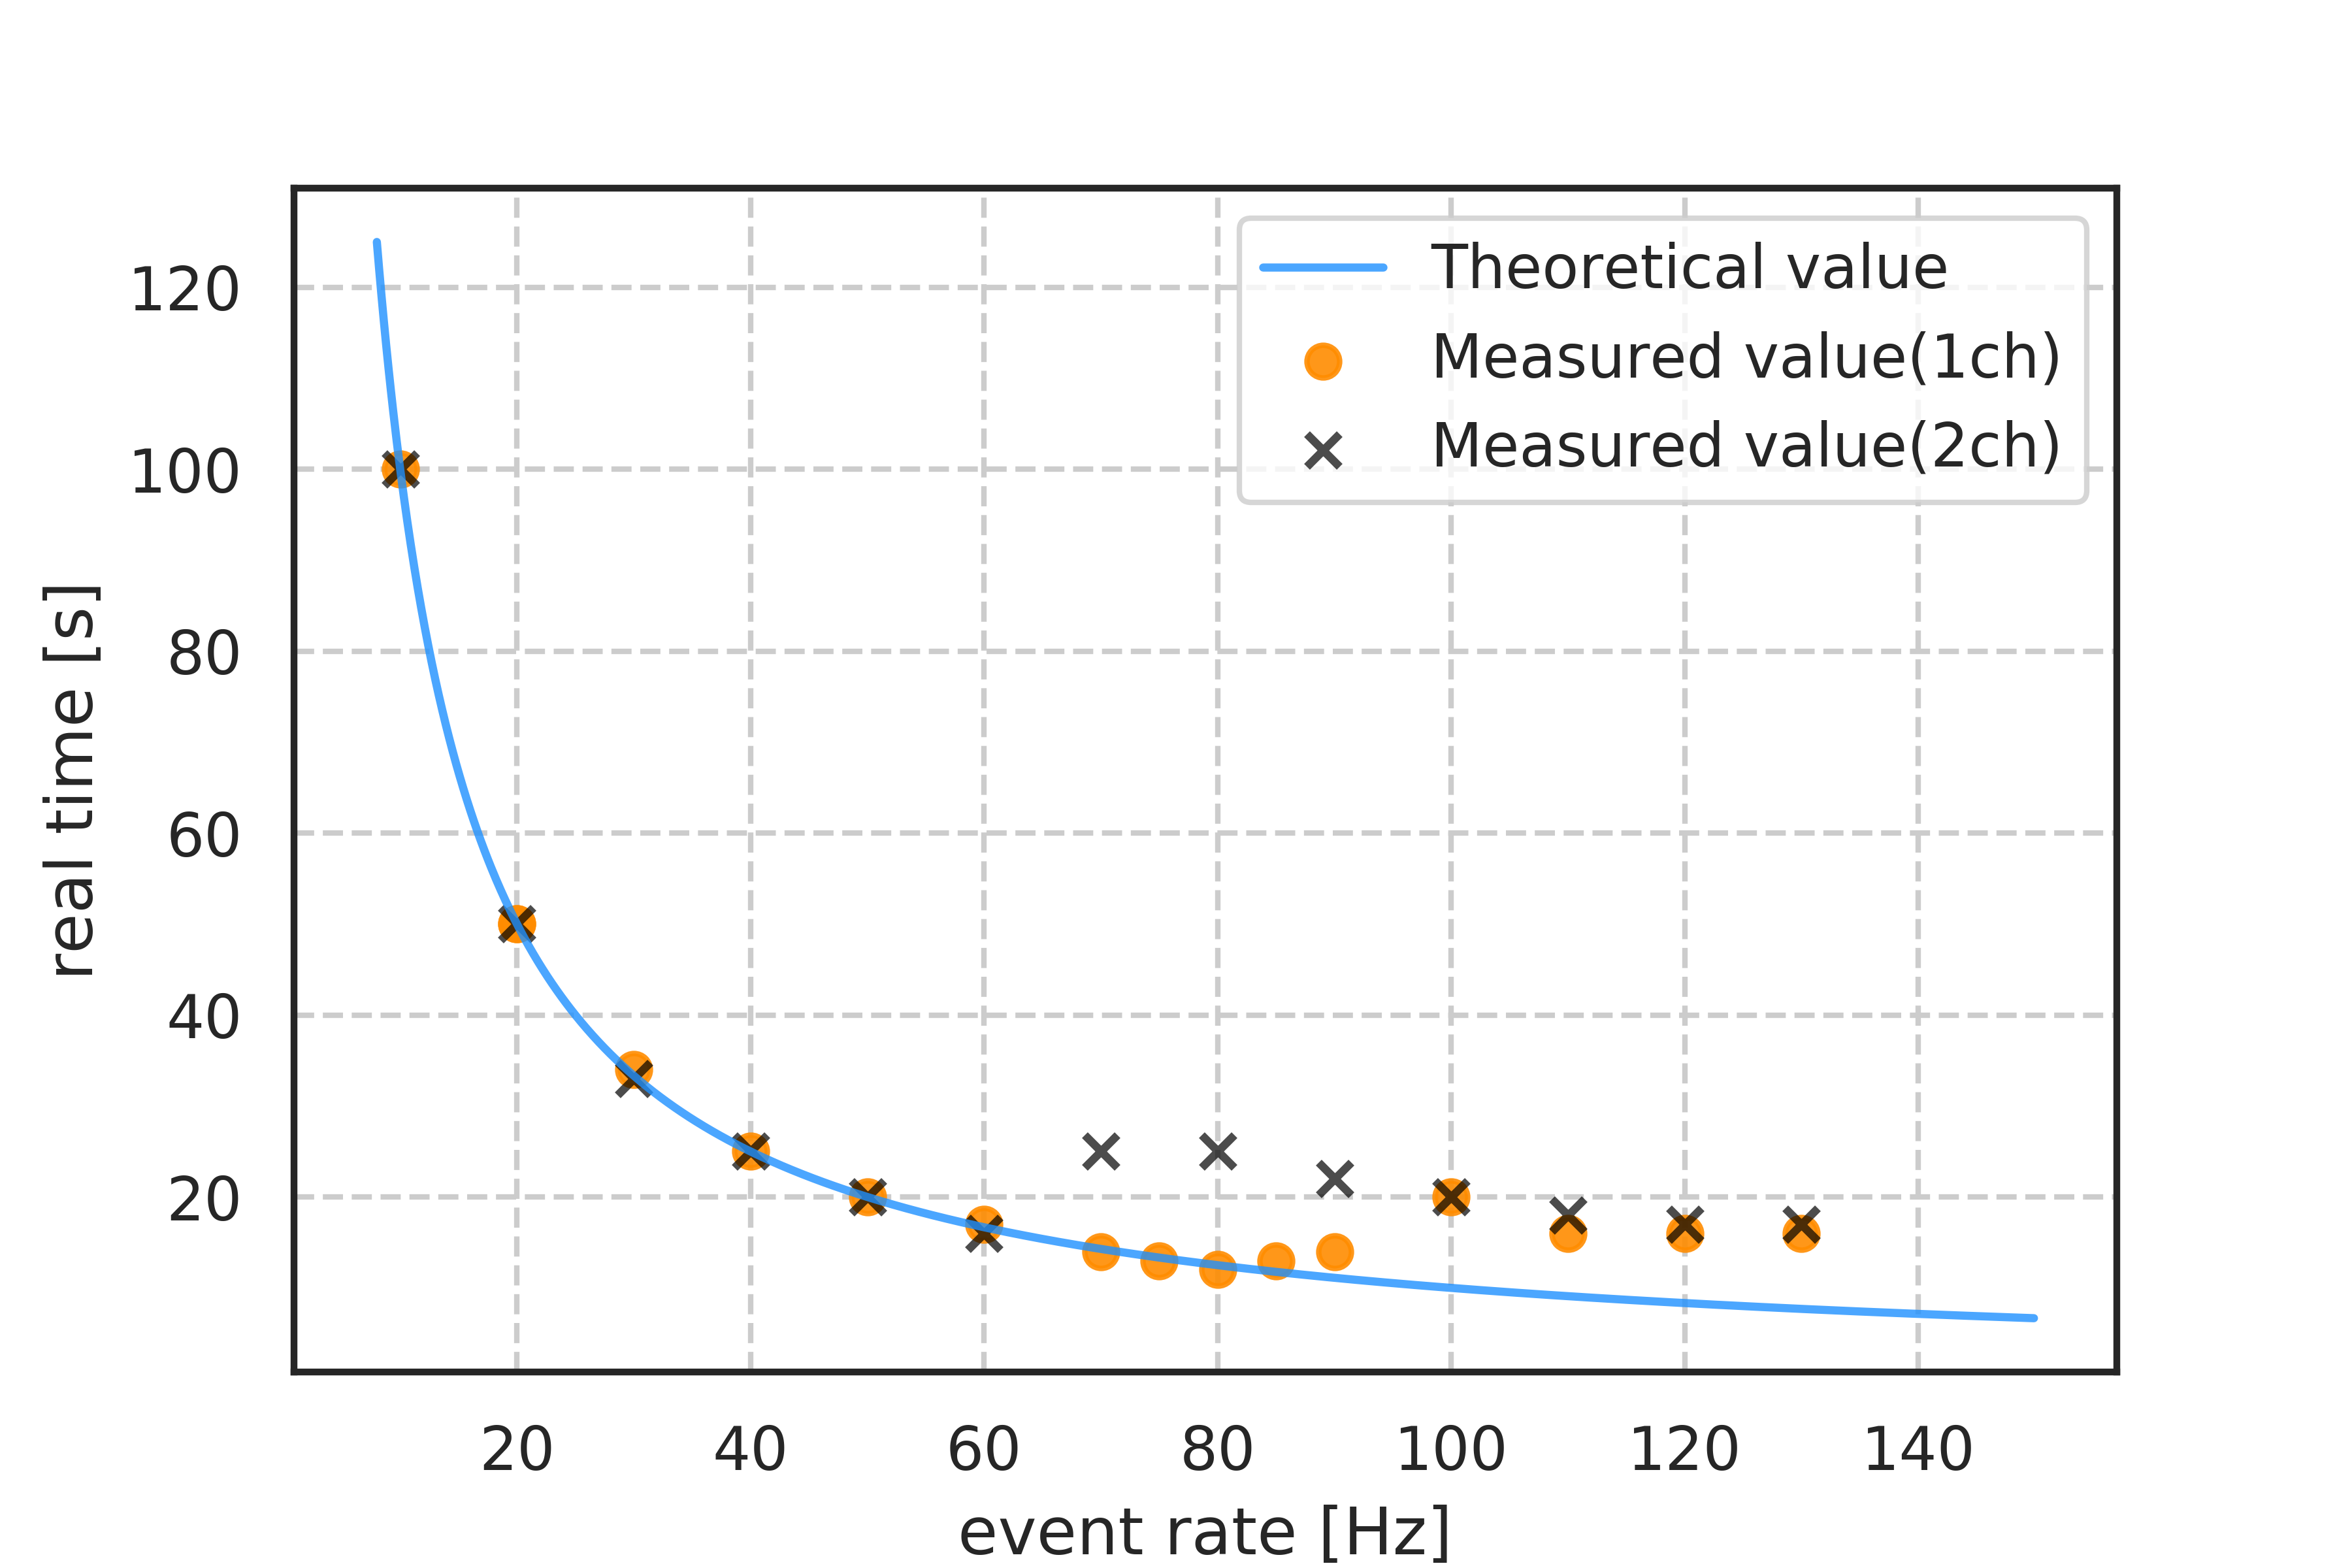
\includegraphics[width=120mm]{picture/daq/trigger_test.png}
\caption{トリガーレートの検証}
\label{trigger}
\end{figure}

\vspace*{5mm}
\noindent
炭素原子核を標的とした場合の、散乱角$40^\circ$における散乱陽子の検出器への入射レートを\eqref{eq:expcs}式を用いて求めた。[表\ref{Rate}]

\begin{table}[h]
   \caption{散乱陽子の予想入射レート}
   \centering
   
\begin{tabular}{cc} \hline
  電流値 [nA] &入射レート [Hz] \\ \hline
  
  \begin{tabular}{c}
    0.1  \\
    1 \\
    10 \\
    100 \\
   \end{tabular} &
   
     \begin{tabular}{c}
    42 \\
    4.2$\times$${10}^2$ \\
    4.2$\times$${10}^3$ \\
    4.2$\times$${10}^4$ \\
   \end{tabular} 
   \\ \hline
   \end{tabular}
   \label{Rate}
\end{table}

\vspace*{5mm}

以上から、電流値の設定や散乱角によっては100Hzを超えるレートでトリガーがかかると予想される。散乱断面積の値を求めるには散乱された粒子の数を正確に求める必要があること、コインシデンスを取る必要がないことから、散乱断面積を求めるための計測にはMCAを用いることとした。MCAはAMP TEK社のMCA8000D(最大トリガーレート:100 MHz)を使用した。

\vspace*{15mm}

\begin{figure}[H]
\centering
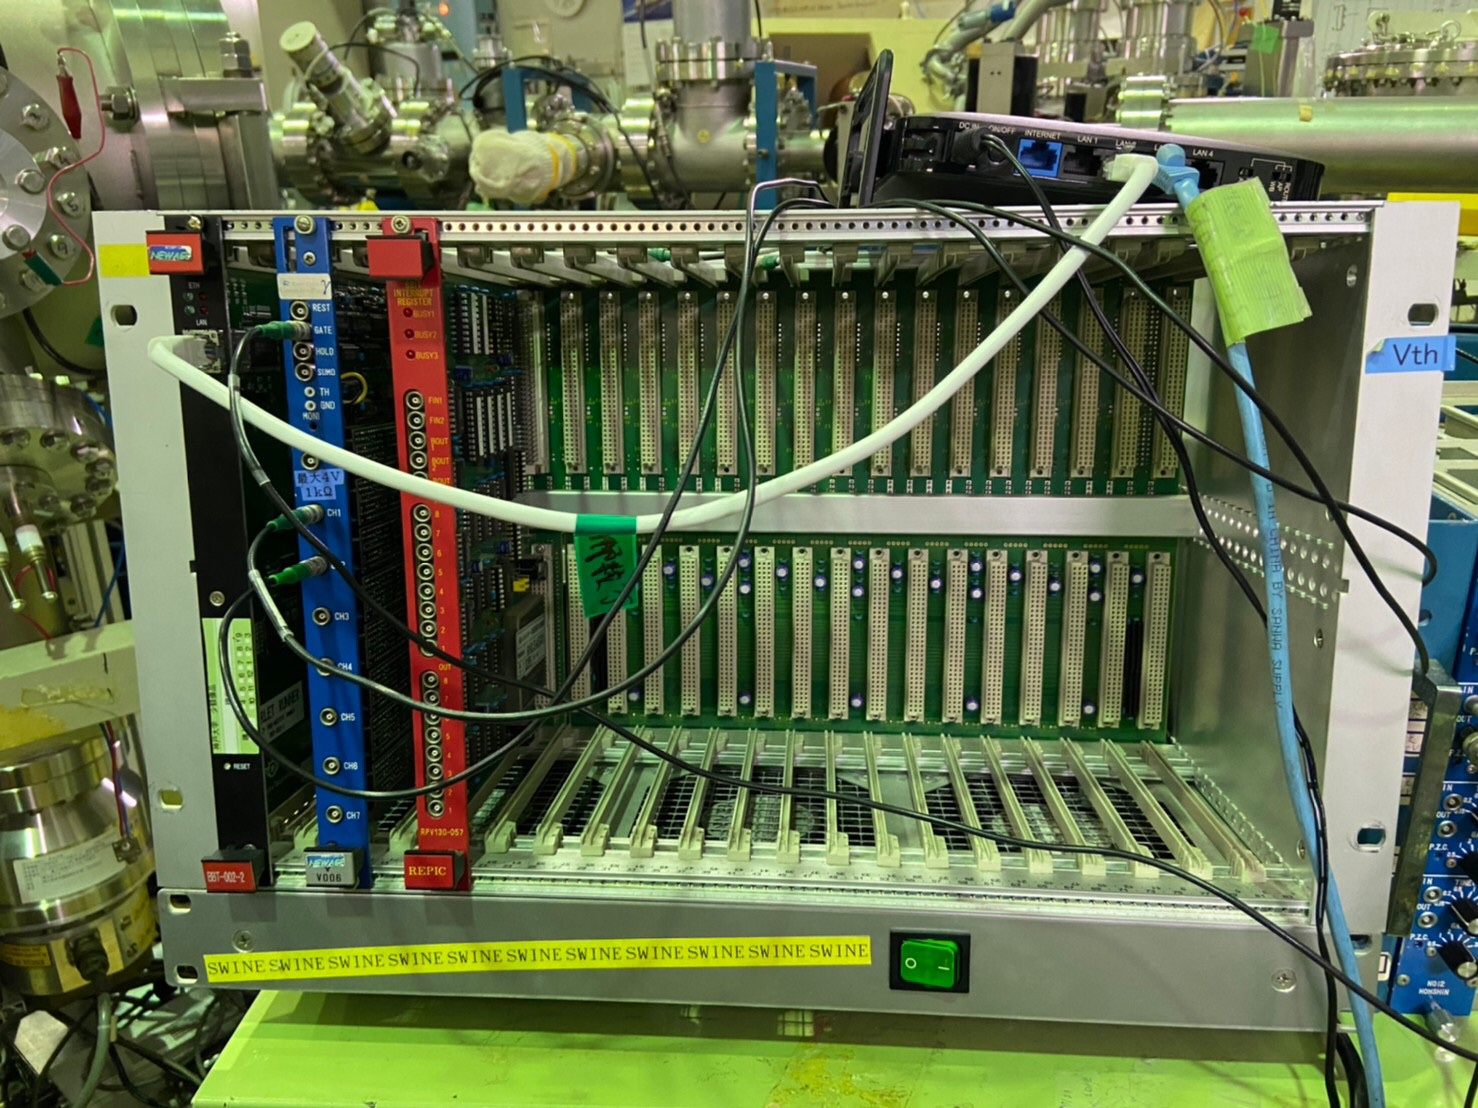
\includegraphics[width=120mm]{picture/daq/vme.JPG}
\caption{使用したVMEクレートとモジュール}
\label{vme}
\end{figure}

\newpage



\end{document}
\documentclass[a4paper,11pt,dvipdfmx]{jsarticle}

\usepackage{bm}
\usepackage[dvipdfmx]{graphicx}
\usepackage[dvipdfmx]{color}
\usepackage{ascmac}
\usepackage{siunitx}
\usepackage{otf}
\pagestyle{plain}
\usepackage{float}
\usepackage[dvipdfmx]{hyperref}
\usepackage{pxjahyper}
\usepackage{here}
\usepackage{titlesec}
\titleformat*{\section}{\LARGE\bfseries}
\titleformat*{\subsection}{\normalsize\bfseries}
\usepackage{url}
\usepackage{comment}
\usepackage[table,xcdraw]{xcolor}
\hypersetup{% hyperrefオプションリスト
setpagesize=false,
 bookmarksnumbered=true,%
 bookmarksopen=true,%
 colorlinks=true,%
 linkcolor=blue,
 citecolor=blue,
}

\begin{document}


\subsection{エネルギー較正}
本節は得られたデータからエネルギー校正を行うことを目的とする。また較正されたエネルギースペクトルの分析も行う。本研究でのデータ解析は主に、CERN(欧州原子核研究機関)が開発する解析フレームワークROOTを用いて行った。

\subsubsection{理論値の導出}
エネルギー較正に用いるため、各角度での散乱陽子のエネルギー理論値を求める。
散乱が弾性散乱であると仮定する。入射陽子がターゲット原子核のクーロンポテンシャルの働かない十分遠方から飛んでくるとすると、エネルギー保存則と運動量保存則より以下の式が求められる。


\begin{equation}
\centering
\large
  E = \left( \frac{\cos\theta+\sqrt{\cos\theta^2+A^2-1}}{A+1} \right)^2 E_0
  \label{scatter}
\end{equation}

\vspace*{2mm}

\begin{center}
\begin{small}
  $\it{E}$:散乱後の陽子のエネルギー $E_0$:入射陽子のエネルギー\\
  $\theta$:実験室系の散乱角度[$^\circ$] A:ターゲット原子の質量数
\end{small}
\end{center} 

\vspace*{5mm}
\noindent
式\ref{scatter}より得られた、各ターゲット原子核に散乱された陽子(入射エネルギー:3MeV)のエネルギーの角度依存性を図\ref{angleE}に示す。

\begin{figure}[H]
\centering
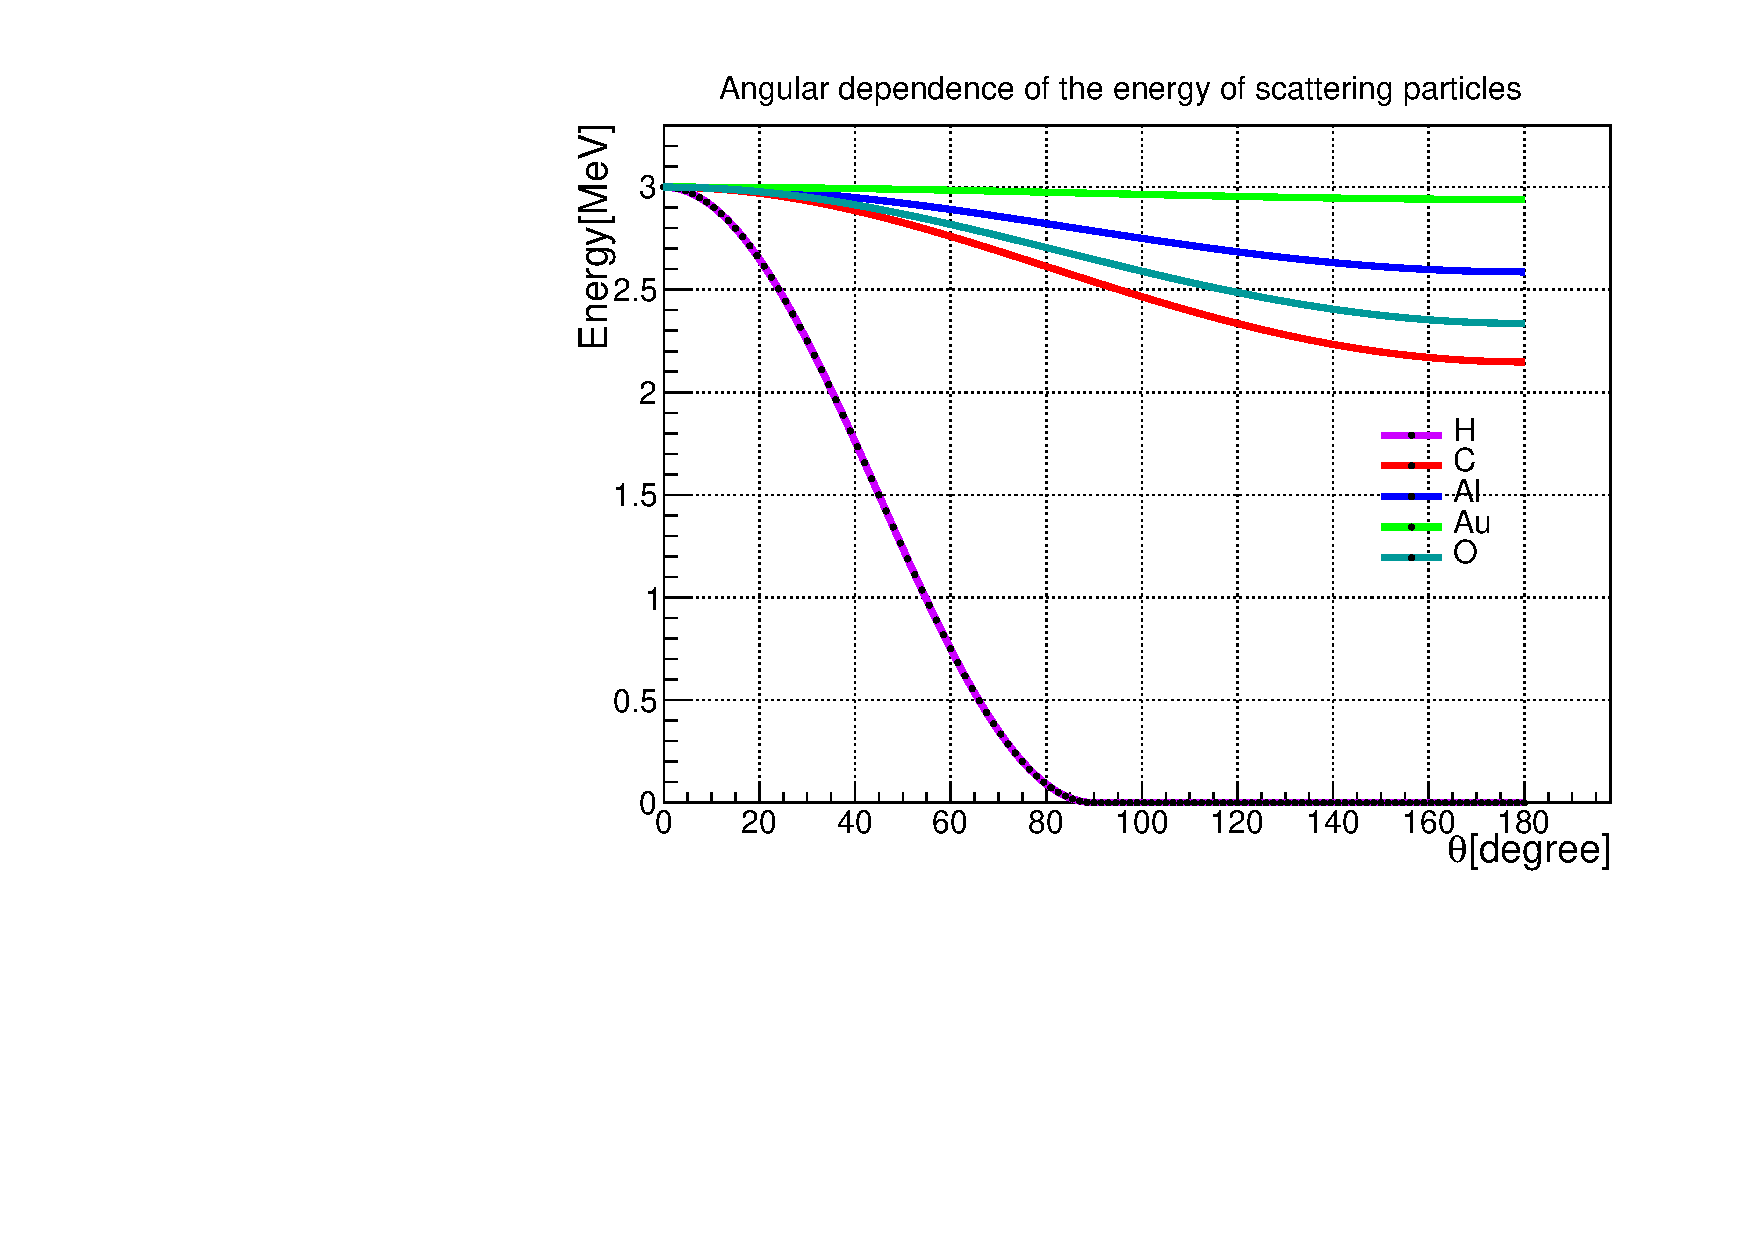
\includegraphics[width=120mm]{picture/cali/protonE.pdf}
\caption{散乱陽子のエネルギーの角度依存性}
\label{angleE}
\end{figure}

\newpage
またターゲットは厚さを持ち、入射粒子や反跳粒子は荷電粒子であることから、Bethe-Blochの式に従いエネルギー損失を起こす。陽子におけるBethe-Blochの式を以下に示す。

\vspace*{2mm}

\begin{equation}
\centering
\large
 -\frac{1}{\rho}\frac{dE}{dx} = \frac{4\pi{N_A}}{{m_e}c^2}{\left( \frac{e^2}{4\pi\varepsilon_0}\right)}^2\frac{Z}{A}\frac{1}{\beta^2}\left[\ln{\left(\frac{2m_ec^2\beta^2}{I(1-\beta^2)} \right)-\beta^2}\right]
  \label{BB}
\end{equation}

\vspace*{2mm}

\begin{center}
\begin{small}
 $\rho$:ターゲットの密度[kg/m$^3$] $N_A$:アボガドロ数[/mol] \\
 \vspace*{1mm}
  $m_e$:電子の質量[eV/c$^2$] c:光速[m/s] \\
  %\vspace*{0.5mm}
  e:電気素量[C] $\varepsilon_0$:真空の誘電率 \\
  \vspace*{0.5mm}
  Z:ターゲットの原子番号 $\beta=\frac{v}{c}:陽子の相対速度$ \\
 %\vspace*{0.3mm}
  $I\simeq16\cdot{Z^{0.9}}$:平均イオン化ポテンシャル[eV]
\end{small}
\end{center}

\noindent
以上の2つの式を用いてエネルギーの理論値を求めた。次節ではその値から予想されるエネルギースペクトルとの比較を行う。\\

\subsubsection{エネルギースペクトルの分析}
各角度でのエネルギースペクトルの分析を行なった。エネルギーの測定値は正規分布に従うと考えられるので、各ターゲット原子核に散乱された陽子はエネルギースペクトル上にピークとして現れる。各ピークとエネルギー理論値との対応を考えた。ここではいくつかの例を示す。\\

\begin{itemize}
  \item 標的が金箔のとき\mbox{}\\
  金原子核を標的としたときのエネルギースペクトルには、総じて1つのピークが見られた。図\ref{angleE}より、金原子核に散乱された陽子のエネルギーは角度による変化が小さいことが分かる。本研究でもその傾向が見られたので、散乱陽子のピークだと結論づけた。30$^{\circ}$と140$^{\circ}$におけるスペクトルをそれぞれ図\ref{Au30}、図\ref{Au140}に示す。
  
   \begin{figure}[H]
    \begin{tabular}{cc}
      \begin{minipage}[t]{0.45\hsize}
        \centering
        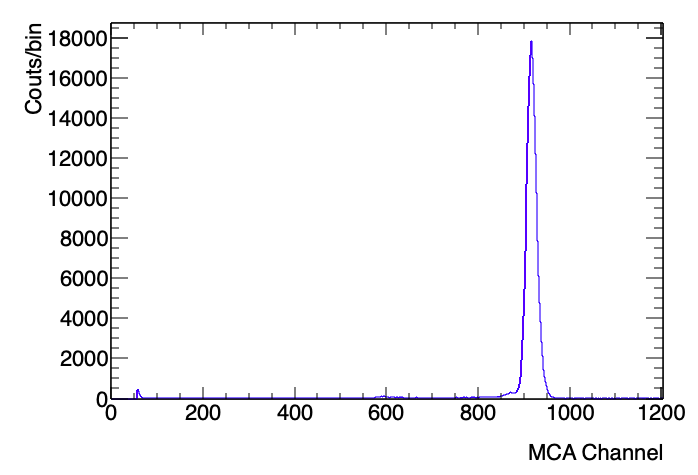
\includegraphics[width=60mm,height=42mm]{picture/cali/Au30.png}
        \caption{30$^{\circ}$におけるスペクトル(MCA)}
        \label{Au30}
      \end{minipage} &
      \begin{minipage}[t]{0.45\hsize}
        \centering
        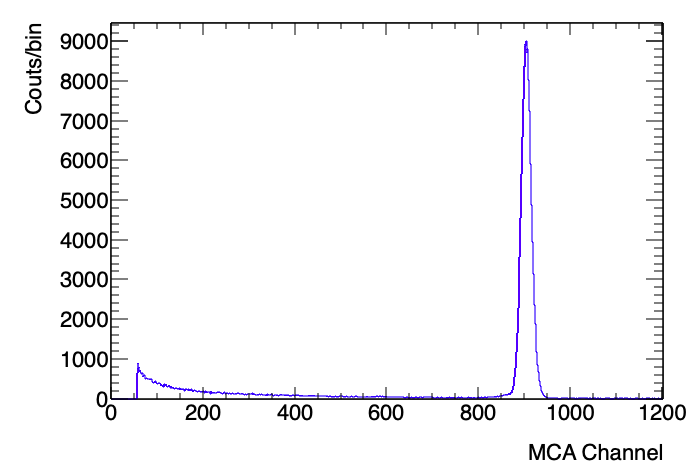
\includegraphics[width=60mm,height=42mm]{picture/cali/Au140.png}
        \caption{140$^{\circ}$におけるスペクトル(MCA)}
        \label{Au140}
      \end{minipage}
    \end{tabular}
  \end{figure}
  
  \item 標的がポリエチレンのとき(低角度)\mbox{}\\
  ポリエチレンの組成式は $(\text{CH}_2)_n$ で表される。図\ref{angleE}より、低角度($\theta\leq90^{\circ}$)では炭素原子核に散乱された陽子のエネルギーは水素原子核によるものよりも大きく、角度と共にその差は大きくなっていく。従って角度が大きくなるにつれて分離されたピークが見られると予想でき、そのような様子が見られた。[図\ref{PE30}] [図\ref{PE60}]\\
  
   \begin{figure}[H]
    \begin{tabular}{cc}
      \begin{minipage}[t]{0.45\hsize}
        \centering
        \includegraphics[width=60mm,height=42mm]{picture/cali/adc30.pdf}
        \caption{30$^{\circ}$におけるスペクトル(ADC)}
        \label{PE30}
      \end{minipage} &
      \begin{minipage}[t]{0.45\hsize}
        \centering
        \includegraphics[width=60mm,height=42mm]{picture/cali/PE60.png}
        \caption{60$^{\circ}$におけるスペクトル(MCA)}
        \label{PE60}
      \end{minipage}
    \end{tabular}
  \end{figure}
  
  60$^{\circ}$のエネルギースペクトルにおいて水素原子核由来のピークはガウス関数の低エネルギー側が潰れたような形をしている。これは粒子のエネルギーが低いためMCAのペデスタルにかかってしまっているからであると考えられる。\\
  
  
  \item 標的がポリエチレンのとき(大角度)\mbox{}\\
  エネルギー保存則と運動量保存則より、水素原子核に衝突した陽子と反跳水素原子核は、大角度($\theta>90^{\circ}$)には散乱されない。従って、炭素原子核に散乱された陽子のピークのみが見られると予想できる。
  
\begin{figure}[H]
\centering
\includegraphics[width=80mm]{picture/cali/PE140.png}
\caption{140$^{\circ}$におけるスペクトル(MCA)}
\label{PE140}
\end{figure}

図\ref{PE140}は140$^{\circ}$におけるエネルギースペクトルである。大角度においてはこのような、ガウシアンに比べてエネルギー分布が広がった形のピークが見られた。これは陽子が入射してから検出器に到達するまでの間の経路差によるものであると考えられる。大角度の散乱では、散乱イベントが発生したターゲット内の位置によってエネルギー損失量に大きな差が生じる。表\ref{Edepo}に30$^{\circ}と140^{\circ}$における、経路の差によって生じるエネルギーの差の最大値を示す。大きな角度で散乱された粒子はターゲット内を進む距離が大きく異なるものが観測されるので、エネルギー分布が図\ref{PE140}のようになると推測される。\\

\begin{table}[h]
\centering
\caption{経路の差によるエネルギーの差}
\begin{tabular}{cccc} \hline
  角度 [$^\circ$] & 最大エネルギー [MeV] & 最小エネルギー [MeV] & エネルギー差 [MeV] \\ \hline
  30 & 2.72 & 2.67 & 0.05 \\ 
  140 &  2.23 & 1.75 & 0.48 \\ \hline
  \label{Edepo}
  \end{tabular}
  \centering
\end{table}

%大きな角度で散乱された粒子はターゲット内を進む距離が大きく異なるものが観測されるので、エネルギー分布が図\ref{PE140}のようになると推測される。

\vspace*{8mm}

\begin{figure}[H]
\centering
\includegraphics[width=140mm]{picture/cali/d.png}
\caption{散乱角度による経路差 \protect \footnotemark}
\label{dis}
\end{figure}

\footnotetext{陽子イラストはひっぐすたんHPより\\ \url{https://higgstan.com}}

\end{itemize}

\newpage
\subsubsection{較正曲線}
本節では、前節で行ったエネルギースペクトルの分析の結果からエネルギー較正を行う。表\ref{ch1cali}、表\ref{ch2cali}、表\ref{mcacali}にエネルギー較正に用いたデータを示す。各ピークをガウシアンでフィッティングし、Mean値をエネルギー理論値と対応させた。

\begin{table}[h]
\centering
\caption{PHADCのchannel1のエネルギー較正}
\begin{tabular}{cccc} \hline
  ターゲット原子核 & 角度 [$^\circ$] & 理論値 [keV] & PHADC channel \\ \hline
  H & 50 & 1188 & 758.2 \\ 
  C & 50 & 2775 & 1814 \\ 
  C & 60 & 2569 & 1738.72 \\ \hline
  \label{ch1cali}
  \end{tabular}
  \centering
\end{table}
\begin{table}[h]
\centering
\caption{PHADCのchannel2のエネルギー較正}
\begin{tabular}{cccc} \hline
  ターゲット原子核 & 角度 [$^\circ$] & 理論値 [keV] & PHADC channel \\ \hline
  H & 30 & 2113.79 & 1426.89 \\ 
  H & 40 & 1598.55 & 1155 \\ 
  C & 30 & 2801.24 & 1743.61 \\ 
  C & 60 & 2569.32 & 1611 \\ \hline
  \label{ch2cali}
  \end{tabular}
  \centering
\end{table}

   \begin{figure}[H]
    \begin{tabular}{cc}
      \begin{minipage}[t]{0.47\hsize}
        \centering
        \includegraphics[width=70mm]{picture/cali/calich1.png}
        \caption{PHADC channel1の較正直線}
        \label{ch1line}
      \end{minipage} &
      \begin{minipage}[t]{0.45\hsize}
        \centering
        \includegraphics[width=70mm,height=49mm]{picture/cali/calich2.png}
        \caption{PHADC channel2の較正直線}
        \label{ch2line}
      \end{minipage}
    \end{tabular}
  \end{figure}

\vspace{2mm}

\noindent  
\begin{center}
channel1 : Energy [keV] = 1.45 $\times$ PHADC\_channel + 87.66 \\
channel2 : Energy [keV] = 2.08 $\times$ PHADC\_channel - 826.98
\end{center} 

\begin{table}[t]
\centering
\caption{MCAのエネルギー較正}
\begin{tabular}{cccc} \hline
  ターゲット原子核 & 角度 [$^\circ$] & 理論値 [keV] & MCA channel \\ \hline
  Au & 30 & 2981.71 & 916.86 \\ 
  Au & 80 & 2957.91 & 911.10 \\ 
  Au & 130 & 2935.97 & 905.39 \\ 
  C & 40 & 2739.97 & 831.72 \\ 
  H & 70 & 332.08 & 95.66 \\ \hline
  \label{mcacali}
  \end{tabular}
  \centering
\end{table}

\begin{figure}[H]
\centering
\includegraphics[width=90mm]{picture/cali/mca_cali.png}
\caption{MCAの較正直線}
\label{mca_cali}
Energy [keV] = 3.19 $\times$ MCA\_channel + 55.92
\end{figure}

以上のようにしてエネルギー較正を行った。以降の解析ではここで行った較正データを用いる。

\vspace*{5mm}

\subsubsection{バックグラウンドの考察}
本実験では、期待されていない事象による信号も観測された。本節ではその原因について考察する。以下の図\ref{PE40_BG}に散乱角度40$^\circ$におけるエネルギースペクトルを示す(標的はポリエチレン)。
p-p散乱によるガウスピークが見られなくなるほどのバックグラウンドが観測された。二次電子抑制管の40$^\circ$と50$^\circ$の間にある穴をなべ頭ネジで埋めたことによる影響であると昨年までは結論づけていたため、本年度は皿頭のものを用いてバックグラウンドの排除を試みたが有意な差は得られなかった。

   \begin{figure}[H]
    \begin{tabular}{cc}
      \begin{minipage}[t]{0.47\hsize}
        \centering
        \includegraphics[width=70mm]{picture/cali/PE40_BG.png}
        \caption{40$^\circ$におけるスペクトル(ADC)}
        \label{PE40_BG}
      \end{minipage} &
      \begin{minipage}[t]{0.45\hsize}
        \centering
        \includegraphics[width=70mm]{picture/cali/PE40_BG2.png}
        \caption{40$^\circ$におけるスペクトル(MCA)}
        \label{PE40_BG2}
      \end{minipage}
    \end{tabular}
  \end{figure}

   \begin{figure}[H]
    \begin{tabular}{cc}
      \begin{minipage}[t]{0.47\hsize}
        \centering
        \includegraphics[width=70mm]{picture/cali/AU110_BG.png}
        \caption{110$^\circ$におけるスペクトル(MCA)}
        \label{AU110_BG}
      \end{minipage} &
      \begin{minipage}[t]{0.45\hsize}
        \centering
        \includegraphics[width=70mm,height=49mm]{picture/cali/AU130_BG.png}
        \caption{130$^\circ$におけるスペクトル(MCA)}
        \label{AU130_BG}
      \end{minipage}
    \end{tabular}
  \end{figure}

\noindent
また100$^\circ\sim120^\circ$の散乱において図\ref{AU110_BG}のような分布も見られた。これはビームストッパーの位置が悪く、陽子を反射してしまったものだと考えられる。130$^\circ$度以上では大幅にバックグラウンドが減少したが、これは検出器がターゲットホルダーの影に隠れたことが原因であると推測される。[図\ref{AU130_BG}]\\

最後に、低角度で見られた期待されなかったピークについて説明する。図\ref{AU20_nazo}のようなピークが金を標的としたときの20$^\circ$、30$^\circ$、ポリエチレンを用いたときの20$^\circ$に見られた。ただし40$^\circ$やポリエチレンのときの30$^\circ$は他の信号に埋れてしまって見えていないと考えられる。
これらのピークの候補としては、反跳された金や炭素の原子核が挙げられる。しかし反跳粒子の散乱断面積は重心系での角度を$\varphi$とすると$\frac{1}{(\cos {\varphi)^3}}$に比例するため\cite{ion}、90度に近づくにつれてより明確にピークが見られるはずである。これらより、反跳原子核によるものではないと結論づけた。

   \begin{figure}[H]
    \begin{tabular}{cc}
      \begin{minipage}[t]{0.47\hsize}
        \centering
        \includegraphics[width=70mm]{picture/cali/AU20_nazo.png}
        \caption{20$^\circ$におけるスペクトル(MCA)}
        \label{AU20_nazo}
      \end{minipage} &
      \begin{minipage}[t]{0.45\hsize}
        \centering
        \includegraphics[width=70mm]{picture/cali/AU20_nazo2.png}
        \caption{図\ref{AU20_nazo}を拡大したもの}
        \label{AU20_nazo2}
      \end{minipage}
    \end{tabular}
  \end{figure}
  
\begin{figure}[H]
\centering
\includegraphics[width=110mm]{picture/cali/recoilcs.png}
\caption{微分反跳断面積の角度依存性}
\label{recoilcs}
\end{figure}
%図\ref{fig:recoil}から分かるように、反跳された原子核のエネルギーは炭素や金がターゲットのときは$E < 1  {\rm MeV}$となる。
%しかし、ピークはそれぞれの角度において1.7 MeV$\sim$1.9 MeVの間に見られた。一般に比電離は阻止能に比例するため、PINフォトダイオードの中で同じエネルギーの陽子に対してより多くの電子を電離させた可能性がある。

\vspace*{7mm}
以上のようにバックグラウンドの考察を行ったがいずれも根本的な解決には至っていない。散乱由来のものであるのか確認するために、ターゲットをなくした状態で計測を行うなどの工夫を行うことが改善点として挙げられる。

 %\vspace*{20mm}



\end{document}
\documentclass[a4paper,11pt,dvipdfmx]{jsarticle}

\usepackage{bm}
\usepackage[dvipdfmx]{graphicx}
\usepackage[dvipdfmx]{color}
\usepackage{ascmac}
\usepackage{siunitx}
\usepackage{otf}
\pagestyle{plain}
\usepackage{float}
\usepackage[dvipdfmx]{hyperref}
\usepackage{pxjahyper}
\usepackage{here}
\usepackage{titlesec}
\usepackage{amsmath,amssymb} %北野加筆
\renewcommand{\bibname}{参考文献} %北野加筆
\titleformat*{\section}{\LARGE\bfseries}
\titleformat*{\subsection}{\normalsize\bfseries}
\usepackage[subrefformat=parens]{subcaption}
\usepackage{url}
\usepackage{comment}
\usepackage{docmute}
\setcounter{page}{0}
\usepackage[table,xcdraw]{xcolor}
\hypersetup{% hyperrefオプションリスト
setpagesize=false,
 bookmarksnumbered=true,%
 bookmarksopen=true,%
 colorlinks=true,%
 linkcolor=blue,
 citecolor=blue,
}


\begin{document}

\newpage

\subsection{微分散乱断面積}
ここでは実験で得られたデータから微分散乱断面積を求めるための理論式を導出する。また解析を行う際に行った補正式についても触れる。

\subsubsection{微分散乱断面積の算出}
ここでは物理量を次のように定義する。
\begin{table}[h]
\small
\it
\centering
\begin{tabular}{ll} 

  $d\Omega$:微小立体角 {\rm [sr]} & n:ターゲット原子核の面密度 {\rm [/cm$^2$]}\\
  N:d$\Omega$に散乱された粒子数 & $N_{all}$:全粒子数 \\ 
  d:ターゲットの密度 {\rm[g/cm$^3$]} & t:ターゲットの厚み {\rm[cm]} \\ 
  N$_A$:アボガドロ数 {\rm[/mol]} & r:二次電子抑制管の穴の半径 {\rm[cm]} \\ 
  l:散乱点から検出器までの距離 {\rm[cm]} & I:陽子ビームの電流値 {\rm[A]} \\ 
  T:計測時間 {\rm[s]} & e:素電荷 {\rm[C]}\\
  A:ターゲット原子の質量数 {\rm[g/mol]}
  \label{def1}
\end{tabular}
\end{table}

\noindent
    面密度{\it n}のターゲットに陽子ビームを照射し、{\it d$\Omega$}の範囲で観測することを考える。単位立体角あたりに陽子が散乱される確率は微分散乱断面積と面密度の積で与えられるから、

\begin{equation}
    \centering
    \frac{d\sigma}{d\Omega} \times n \times d\Omega = \frac{N}{N_{all}} 
\end{equation}
と表される。またそれぞれの値は
\begin{eqnarray}
    \centering
    &n = \frac{d \times t \times N_A}{A}&\\
    &d\Omega = \frac{\pi{r^2}}{l^2}&\\
    &N_{all} = \frac{IT}{e}&
\end{eqnarray}

の3式で求められる。これらから、微小立体角$d\Omega$における微分散乱断面積$\frac{d\sigma}{d\Omega}$は\eqref{eq:expcs}式で表すことができる。

\begin{equation}
    \frac{d\sigma}{d\Omega} = \frac{l^2 \times N \times e \times A}{\pi{r^2} \times I \times T \times d \times t \times N_A}
    \label{eq:expcs}
\end{equation}


\newpage
\subsubsection{各パラメーターの決定}
\eqref{eq:expcs}式をもとに、各角度における微分散乱断面積を求める際のパラメーターを決定する。ここではパラメーター決定の方法とそれぞれの誤差について説明する。

\begin{description}
   \item[● 散乱粒子数 ${\it N}$]\mbox{}\\
   エネルギースペクトルの対応するピークを積分することで求めた。スペクトル上にガウスピークが見られる場合はMean値から$\pm3\sigma$の範囲を積分した。3$\sigma$の範囲で積分することで、理論的に99.7\%の粒子数をカウントすることができる。また図\ref{PE140}のような分布に関しては、複数のガウシアンでフィッティングを行うことで$3\sigma$の値を決定し、積分を行った。 
   
   \vspace*{5mm}
   
    \begin{figure}[H]
     \begin{tabular}{cc}
       \begin{minipage}[t]{0.45\hsize}
        \centering
        \includegraphics[width=60mm,height=42mm]{picture/CS/3sigma.png}
        \caption{ガウシアンにおける3$\sigma$}
        \label{3sigma}
       \end{minipage} &
       \begin{minipage}[t]{0.45\hsize}
        \centering
        \includegraphics[width=60mm,height=42mm]{picture/CS/PE120_140_1.pdf}
        \caption{複数のガウシアンによるfitting}
        \label{triplegauss}
       \end{minipage}
     \end{tabular}
   \end{figure}
  また誤差${\it \sigma_N}$ = $\sqrt{N}$ とした。\\
   
  \item[● 電流値 ${\it I}$]\mbox{}\\
   ビームの強度を表す電流値{\it I}は、ビームストッパーと導通している二次電子抑制管に流れる電流値を測定することで決定した。計測は5秒ごとに行い、ビームタイムの中での平均値を実験値とした。計測にはT\&D社のデータロガーを用いた。誤差${\it \sigma_I}$には平均値を最確値とした標準誤差を使用した。\\
  
  \item[● 計測時間{\it T}]\mbox{}\\
   MCAでの計測におけるLive timeを${\it T}$とし、本研究では${\it T}$ = 100 [s]で計測を行った。\\
\end{description}

\newpage
\subsubsection{誤差の算出}
$n$個の変数からなる関数$f(x_1,x_2,\cdots,x_n)$を考える。変数${ x_i}$の誤差$\sigma_{x_i}$が互いに独立であるなら、その関数の誤差$\sigma_f$は\eqref{eq:err1}式のように表される。

\begin{equation}
\centering
\sigma_f = \sqrt{\sum_{i=1}^{n} \left(\frac{\partial f}{\partial x_i} {\sigma_{x_i}}\right)^2}
\label{eq:err1}
\end{equation}

\noindent
本研究では\eqref{eq:expcs}式における誤差を含むパラメーターを $N$、$I$、$d$、$t$と設定した。$g = \frac{d\sigma}{d\Omega}$とし、
それぞれの誤差を伝播させて\eqref{eq:err2}式で算出を行った。

\begin{equation}
\centering
\sigma_g = \sqrt{ \left(\frac{\partial g}{\partial N} {\sigma_N }\right)^2 + \left(\frac{\partial g}{\partial I} {\sigma_I }\right)^2 + \left(\frac{\partial g}{\partial d} {\sigma_d }\right)^2 + \left(\frac{\partial g}{\partial t} {\sigma_t }\right)^2}
\label{eq:err2}
\end{equation}


\subsubsection{角度の補正}
Rutherfordの散乱公式\eqref{eq:Rutherford}における角度$\theta$は重心系である。本実験での計測は実験室系の角度を用いていたため、補正を行う必要がある。変換公式は以下のように与えられる。
\begin{equation}
    \tan \theta_{lab} = \frac{\sin \theta_{cm}}{M_1/M_2 + \cos {\theta_{cm}}}
\end{equation}

\begin{table}[h]
\small
\centering
\begin{tabular}{ll} 
    $\theta_{lab}$:散乱角度(実験室系)[$^\circ$] & $\theta_{cm}$:散乱角度(重心系)[$^\circ$] \\
    $M_1$:入射粒子の質量数 & $M_2$:標的原子の質量数
    \label{def2}
\end{tabular}
\end{table}

\noindent
入射粒子は陽子(水素原子核)であるため、$M_1 = 1$である。標的が金のとき$1/M_2$は十分に小さいため$\theta_{lab} \simeq \theta_{cm}$となるが、炭素原子核や水素原子核がターゲットのときには大きなずれが生じるので補正を行った。水素原子核がターゲットのときは、$\theta_{cm} = 2      \theta_{lab}$で表される。

\subsubsection{散乱公式の補正}\label{kakuhosei}
\eqref{eq:Rutherford}式は入射粒子の質量がターゲット原子核の質量より十分小さいことを条件とするものである。炭素原子核を標的とするとき、その質量比は無視できないので換算質量への補正を行う必要がある。換算質量を$\mu$とすると、
\begin{equation}
\frac{1}{\mu} = \frac{1}{M_1} + \frac{1}{M_2}
\end{equation}
で表される。

\newpage
\subsubsection{核力による散乱の補正}
\ref{NF}節において、核力による散乱における微分散乱断面積を導出した。しかしこれは古典的な導出であるので、ここでは入射粒子を平面波として扱って導出する。物理量を以下のように定義する。
\begin{table}[h]
\small
\it
\centering
\begin{tabular}{ll} 
    R:ターゲット原子核の半径 & $\lambda$:陽子の{\rm de Broglie}波長\\
    h:プランク定数 & k:波数\\
    l:軌道角運動量 & $\delta$:位相差\\
    $\mu$:換算質量 & $\sigma$:全散乱断面積\\
    $m_{p}$:陽子の質量 & p:{\rm3 MeV}の陽子の運動量\\
    $f(\theta)$:散乱角$\theta$における散乱振幅
    
\label{def3}
\end{tabular}
\end{table}

運動する物体は波の性質を持っており、そのde Brogrie波長は(\ref{dB})式のように表される。今回用いたのは3 MeVの陽子であるので、その波長は$\lambda \simeq 16.53$ fmである。\\
\begin{equation}
    \lambda = \frac{h}{p} = \frac{h}{m_{p}v}
    \label{dB}
\end{equation}\\
ここでは入射平面波と反射球面波を部分波展開することで、散乱球面波の位相の変化から散乱断面積を導出する。
%入射平面波と反射平面波の振幅の絶対値は等しくなるはずなので、
%\begin{equation}
 %   |1 + 2ikf_l(\theta)| = 1
%\end{equation}
散乱ポテンシャルV(r)が球対称な場合、散乱振幅はルジャンドル多項式を用いて級数展開することができ、\\
\begin{equation}
    f(\theta) = \sum_{l=0}^{\infty} (2l+1) \: f_l \: P_l (cos\theta) 
\end{equation}\\
のように書ける。ここで$f_l$は部分波振幅である。散乱の前後で粒子の湧き出しや吸い込みはないので、入射波と反射波の振幅は等しくなければならない。$\delta_l$を剛体球がない場合の散乱波とある場合の位相の差とすると、\\
\begin{equation}
    e^{2i\delta_l} = 1 + 2ikf_l
    \label{sinpuku}
\end{equation}\\
と定義される。波動関数の動径方向に関するSchr\"{o}dinger方程式(\ref{sch})を解き、剛体球がない場合の位相と比較を行うと、部分波振幅$f_l$は(\ref{sinpuku})式の結果より(\ref{bubun})式のように与えられる。\\
\begin{equation}\\
    \left[-\frac{\hbar^2}{2\mu}\left\{\frac{d}{dr}-\frac{l(l+1)}{r^2}\right\} + V(r)\right]\psi_l(r) = \frac{\hbar^2k^2}{2\mu}\psi_l(r)
    \label{sch}
\end{equation}
\begin{equation}
    f_l = \frac{e^{i\delta_l}\sin \delta_l}{k}
    \label{bubun}
\end{equation}
以上より、全散乱断面積$\sigma$は(\ref{zendan})式のように表される。
\begin{eqnarray}
    \sigma &=& \int |f(\theta)|^2 d\Omega\\
    &=& \frac{4\pi}{k^2}\sum_{l}(2l+1)\sin^2 \delta_l
    \label{zendan}
\end{eqnarray}

\noindent
核力による散乱を剛体球による散乱と仮定すると、その散乱ポテンシャル$V(r)$は剛体球の中心を原点とした座標rを用いて\\
\begin{equation}
    V(r) = \begin{cases}
    \infty & (r < R)\\
    0 & (r > R)
    \end{cases}
\end{equation}\\
のように表される。剛体球の中には入射平面波は侵入できないので、$r=R$で$\psi=0$となる。したがって位相差$\delta_l$は、
\begin{eqnarray}
    kR + 2\delta_l &=& -( kR - \pi l)\\
   \delta_l &=& \frac{\pi l}{2} - kR 
\end{eqnarray}
のように表される。$k=\frac{2\pi}{\lambda}$より、入射平面波の波長$\lambda$とポテンシャルの及ぶ範囲$R$の相対的な関係により位相差$\delta_l$が変化することがわかる。ここで、$\lambda$が$R$に対して十分に大きい場合を考えると、$l=0$の成分(S波)のみを考えればよく、$\delta_l=-kR$となる。したがって全断面積$\sigma$は(\ref{sigma})式で表される。またS波は等方的に散乱されるため、核力による微分散乱断面積は、(\ref{kakubibun})式で与えられる。\\
\begin{equation}
    \sigma = \frac{4\pi}{k^2}\sin^2 {\delta_l}
    \label{sigma}
\end{equation}
\begin{equation}
   \frac{d\sigma}{d\Omega} = \left(\frac{\sin \delta_l}{k}\right)^2
   \label{kakubibun}
\end{equation}\\
ここで$\delta_l \ll 1$とすると、$\sin \delta_l \simeq \delta_l$と近似できるので\eqref{eq:NFcs}式のように表され、幾何学的に求めた古典的な散乱断面積(\ref{eq:nfcr2})の4倍となることが分かる。\\
\begin{equation}
    \frac{d\sigma}{d\Omega} \simeq R^2
    \label{eq:NFcs}
\end{equation}

\end{document}
\documentclass[a4paper,11pt,dvipdfmx]{jsarticle}

\usepackage{bm}
\usepackage[dvipdfmx]{graphicx}
\usepackage[dvipdfmx]{color}
\usepackage{ascmac}
\usepackage{siunitx}
\usepackage{otf}
\pagestyle{plain}
%\usepackage[subrefformat=parens]{subcaption}
\usepackage{float}
\usepackage[dvipdfmx]{hyperref}
\usepackage{pxjahyper}
\usepackage{here}
\usepackage{titlesec}
\titleformat*{\section}{\LARGE\bfseries}
\titleformat*{\subsection}{\normalsize\bfseries}
\usepackage{url}
\usepackage[table,xcdraw]{xcolor}
\hypersetup{% hyperrefオプションリスト
setpagesize=false,
 bookmarksnumbered=true,%
 bookmarksopen=true,%
 colorlinks=true,%
 linkcolor=blue,
 citecolor=blue,
}


\begin{document}
\newpage
\section{\LARGE{議論と考察(担当:木村)}}

\subsection{目的}
本章ではこれまでの解析から得られた微分散乱断面積の評価を行う。炭素においては核力による微分散乱断面積から原子核半径の推定を行う。また2つの検出を用いた2チャンネル同時計測により、p-p散乱の観測を試みる。

\subsection{微分散乱断面積の評価}
\subsubsection{文献値との比較}
本実験では金とポリエチレン(水素と炭素)をターゲットとして用い、それらの微分散乱断面積を導出した。微分散乱断面積の文献値はRutherfordの公式より
\begin{equation}
    \frac{d\sigma}{d\Omega} = \left(\frac{Z_1Z_2e^2}{16\pi\epsilon_0E}\right)^2\frac{1}{\sin^4{\frac{\theta}{2}}}
    \label{siki1}
\end{equation}
で表される。この文献値はクーロン力のみを考慮しているため、金に対して考察を行う。その際に、測定値に fit 線を引くことにより文献値との比較を行う。具体的には
\begin{equation}
    (fit線) = [p_0] \times \left(\frac{Z_1Z_2e^2}{16\pi\epsilon_0E}\right)^2\frac{1}{\sin^4{\frac{\theta}{2}}}
    \label{crosssection}
\end{equation}
という式をfittingに用いる。この式は式(\ref{siki1}) に定数 p0 をかけており、p0をパラメーターとして動かし、測定値に最小二乗法を用いてfitさせる。この線を引くことで、fit 線に測定値が乗っているかどうかを評価する。また p0 が1に近いほど文献値と一致していると言えるので、その点も評価対象とする。
\subsubsection{金の微分散乱断面積}
まずは核力の影響しないターゲットである金の微分散乱断面積から考察していく。図\ref{aucs}に微分散乱断面積の測定値、文献値、fit線を示す。パラメータ p0 はほとんど 1 に近く、測定点は fit 線によく乗っている。ただし、110$^{\circ}$の点については除外している。その理由については次節で記述する。また100$^\circ$と120$^\circ$の点についてもノイズが少しはいっていたが、110$^\circ$の点に比べ、ノイズが小さかったので残した。
\begin{figure}[H]
\centering
\includegraphics[width=100mm]{picture/jan/Au_CM.pdf}
\caption{金の微分散乱断面積}
\label{aucs}
\end{figure}

図\ref{sp110}は測定角度110$^\circ$のスペクトルである。ノイズがはいっており、散乱陽子数を精度良く求められない。測定角度70$^\circ$のスペクトル(図\ref{sp70})と比較するとノイズがはいってきているのは明らかである。このノイズはターゲットにより散乱されたものではなく、ターゲットホルダーなどの別の物質によって散乱された陽子が観測されているものと考えられる。微分散乱断面積は以下の式で算出する。\\\\
\begin{equation}
    \frac{d\sigma}{d\Omega} = \frac{N\times e \times A}{d\Omega \times I \times T \times d \times t \times N_A}
    \label{expcross}
\end{equation}\\
微分散乱断面積は散乱陽子数に依り、110$^\circ$の点を含めると正確な算出が困難になるため、今回は除外した。\\\\
\begin{figure}[H]
\begin{minipage}{0.5\hsize}
\begin{center}
\includegraphics[width=70mm]{picture/jan/110hist.png}
\end{center}
\caption{110$^\circ$におけるスペクトル}
\label{sp110}
\end{minipage}
\begin{minipage}{0.5\hsize}
\begin{center}
\includegraphics[width=70mm]{picture/jan/70hist.png}
\end{center}
\caption{70$^\circ$におけるスペクトル}
\label{sp70}
\end{minipage}
\end{figure}
\subsubsection{炭素の微分散乱断面積}\label{C1}
炭素の微分散乱断面積の導出にはポリエチレンをターゲットとして用いている。また炭素の場合は陽子が原子核に達することがあるので、クーロン力だけでなく核力による散乱も考慮する必要がある。この時の文献値は\ref{NF}より、
\begin{equation}
    \frac{d\sigma}{d\Omega} = \left(\frac{Z_1Z_2e^2}{16\pi\epsilon_0E}\right)^2\frac{1}{\sin^4{\frac{\theta}{2}}} + \frac{R^2}{4}
\end{equation}
となる。したがって、炭素の微分散乱断面積のfittingはこの式を用いて行う。この核力による微分散乱断面積を用いて原子核半径の推定も行う。図\ref{tanso1}に炭素の微分散乱断面積の測定値、文献値、fit線を書いている。理論値とのズレが大きく、ポリエチレンの炭化によって厚さ・密度が変化している可能性が考えられる。次節において炭化による厚さと密度の変化量を見積もる。
\begin{figure}[H]
\centering
\includegraphics[width=100mm]{picture/jan/C1.png}
\caption{炭素の微分散乱断面積}
\label{tanso1}
\end{figure}
\subsubsection{炭化の考慮}
先行研究\cite{2019}よりポリエチレンは無酸素状態で熱することで炭化し、炭化した場合の密度はしない場合の約2倍であることがわかっていた。ポリエチレンが炭化したことにより(\ref{expcross})式の $d \times t$ の値が変化し、微分散乱断面積にズレが生じていので厚さ・密度の再測定を行った。$\alpha$線のエネルギーを、ターゲットに当てた場合とターゲットなしの場合で比較し、Bethe-Blochの式を用いてエネルギー損失から$d \times t$の推定を行った。その結果、以下の値が得られた。
\begin{equation}
d\times t = (1.61\pm 0.02)\times 10^{-3} \:\: \text{(g/cm$^2$)}
\end{equation}
この値は炭化を考慮する前と比較すると2倍程度ずれていることが分かる。図\ref{tanka1}に炭化を考慮した炭素の微分散乱断面積の測定値、文献値、fit線を示す。
\begin{figure}[H]
\centering
\includegraphics[width=110mm]{picture/jan/C2.png}
\caption{炭素の微分散乱断面積(炭化を考慮)}
\label{tanka1}
\end{figure}

\label{C2}
炭素の原子核半径の推定には炭化を考慮した図\ref{tanka1}を用いる。グラフより
\begin{equation}
\frac{R^2}{4} = (6.54\pm 1.92)\times 10^{-26} \text{cm}^2
\end{equation}
これより
\begin{equation}
R = 5.12\pm 0.75\ \text{fm}
\end{equation}
この時、$R$は原子核半径と陽子半径の和であるから、陽子半径 0.87 fm を引いて
\begin{equation}
r_c = 4.25\pm 0.75\ \text{fm}
\label{tankasiki}
\end{equation}

\newpage
\subsubsection{核力の補正と考察}
\ref{C1}、\ref{C2}節で行った解析は核力による散乱断面積を古典的に導出したものを使用していた。ここで\ref{kakuhosei}節で述べたように量子論を考慮した散乱断面積を導入する。炭素の原子核半径は表\ref{table:gensi}より、$r_c=2.97 $ fmであることを用いて補正を行った。[図\ref{c_cs_hosei}]
\begin{figure}[H]
    \centering
        \includegraphics[width=110mm]{picture/jan/C5.png}
    \caption{炭素の微分散乱断面積(核力の補正あり)}
    \label{c_cs_hosei}
\end{figure}
図\ref{tanka1}と比較してfitting関数がより実験値に近づいていることが分かる。ここで、fittingパラメータp0 $= 0.76 \pm 0.04$であった。またfittingによって得られた核力による微分散乱断面積は、
\begin{equation}
    \frac{d\sigma}{d\Omega} = \left( 1.081 \pm 0.109 \right) \times 10^{-25} \:cm^2/sr
\end{equation}
であった。\ref{kakuhosei}節より$\frac{d\sigma}{d\Omega}=R^2$と近似できるのでこれを用いて原子核半径を求めると
\begin{equation}
    R = 3.29 \pm 0.05 \: fm
\end{equation}
と算出され、\ref{tankasiki}式より理論値2.97 fmに近づいたものの、誤差の範囲内には収まらなかった。これは\ref{kakuhosei}節における近似によるものであると考えられる。まず、S波のみが散乱断面積に寄与するのは$\lambda \gg R$の条件下である。今回入射波長は$\lambda=16.52\:$fmであるため、$\lambda \gg R$とは言い難い。そのため正確な断面積の導出には、$l\geq1$における散乱振幅を考えなければならない。また$\frac{d\sigma}{d\Omega}=R^2$の関係式も同様の条件のもとでの近似式であるので、厳密には異なる。

\newpage
\subsubsection{水素の微分散乱断面積}
続いて、水素の散乱断面積を求めた。図\ref{expmott}に水素を標的とした際の散乱断面積とfitting曲線、そして理論値を示す。
\begin{figure}[H]
\centering
\includegraphics[width=100mm]{picture/jan/H2.png}
\caption{水素の微分散乱断面積}
\label{expmott}
\end{figure}
図\ref{expmott}より、散乱断面積の実測値は理論値と比較してオーダー1つ大きいような結果となった(fittingパラメータ p0$=47.28$)。原因として考えられるのは、Mottの散乱公式(\ref{eq:Mott})に対して、核力による散乱が本研究で考慮している理論値より多くはたらいていることが挙げられる。\ref{kakuhosei}の核力は異種粒子間の散乱を前提としていること、反跳水素原子核についても散乱断面積を導出していないことが原因として考えられる。それらの考慮を行うことでMott散乱のより正確な測定や、水素原子核(陽子)の半径を求めることができると考えた。


\newpage
\subsection{p-p散乱}
\subsubsection{p-p散乱の観測}
\ref{opening}節よりp-p散乱の opening angle は非相対論では90$^{\circ}$であるから、その観測においてp-p散乱が見られるかどうかを考えていく。角度のとり方を図\ref{kakudo}に示す。図\ref{4050}は40$^{\circ}$と50$^{\circ}$における2つの検出器でのエネルギーの相関を表した二次元ヒストグラムである。図\ref{fig:scaene}と図\ref{fig:recoil}よりそれぞれのエネルギーを対応させると、この二次元ヒストグラムからコインシデンスが上手くとれていることが分かるので、40$^{\circ}$と50$^{\circ}$の同時計測ではp-p散乱が見ることができたと結論づけた。
\begin{figure}[H]
    \begin{tabular}{cc}
      \begin{minipage}[t]{0.45\hsize}
        \centering
        \includegraphics[width=70mm]{picture/jan/kakudo.png}
        \caption{角度のとり方}
        \label{kakudo}
      \end{minipage} &
      \begin{minipage}[t]{0.45\hsize}
        \centering
        \includegraphics[width=70mm]{picture/jan/4050.png}
        \caption{40$^{\circ}$と50$^{\circ}$の同時計測(CH1が50$^\circ$、CH2が40$^\circ$)}
        \label{4050}
      \end{minipage}
    \end{tabular}
\end{figure}
また図\ref{hist3060}、図\ref{hist2070}はそれぞれ30$^{\circ}$と60$^{\circ}$、20$^{\circ}$と70$^{\circ}$の2つの検出器でのエネルギーの相関を表した二次元ヒストグラムである。表\ref{rironchi}より、予想されるエネルギー帯においてコインシデンスがとれておらず、p-p散乱を観測できていないということが分かる。60$^{\circ}$や70$^{\circ}$のような大角度はp-p散乱が見られなかった。また理論値と異なるだけでなく、観測されたイベントレートも非常に小さかったため、これらの信号は偶発的なものである可能性が高い。

\vspace*{7mm}

\begin{table}[h]
   \caption{p-p散乱におけるエネルギー理論値(標的中でのエネルギー損失は考慮していない)}
   \centering
 \begin{tabular}{cc} \hline
  散乱角度のペア [$^\circ$] & エネルギー理論値 [MeV] \\ \hline \hline
  
  \begin{tabular}{c}
    40 - 50  \\
    30 - 60 \\
    20 - 70 \\
   \end{tabular} &
   
  \begin{tabular}{c}
    1.76 - 1.24 \\
    2.25 - 0.75 \\
    2.65 - 0.35 \\
  \end{tabular} 
   \\ \hline
   \end{tabular}
   \label{rironchi}
\end{table}

\begin{figure}[H]
    \begin{tabular}{cc}
      \begin{minipage}[t]{0.45\hsize}
        \centering
        \includegraphics[width=70mm]{picture/jan/3060.png}
        \caption{30$^{\circ}$と60$^{\circ}$の同時計測(CH1が60$^\circ$、CH2が30$^\circ$)}
        \label{hist3060}
      \end{minipage} &
      \begin{minipage}[t]{0.45\hsize}
        \centering
        \includegraphics[width=70mm]{picture/jan/2070.png}
        \caption{20$^{\circ}$と70$^{\circ}$の同時計測(CH1が70$^\circ$、CH2が20$^\circ$)}
        \label{hist2070}
      \end{minipage}
    \end{tabular}
\end{figure}


大角度においてp-p散乱が見られなかった原因として、60,70$^\circ$における信号がディスクリミネーターのthresholdよりも小さく、パルスが出力されていなかった可能性が挙げられる。そこでパルスジェネレーターを用いて、PHADCの値を電圧に換算することでthreshold電圧と比較した。図\ref{PHADC_V}はPHADCの値と電圧の換算直線、60$^{\circ}$と70$^{\circ}$におけるPHADCの理論値、ディスクリミネーターのthreshold電圧を示したグラフである。thresholdはおよそ100mVであり、グラフより60$^{\circ}$および70$^{\circ}$のPHADCの値は電圧に換算するとthresholdよりも低いことが分かる。したがって、このことが原因でp-p散乱が見られなかったと言える。\\
 20-70$^\circ$、30-60$^\circ$の計測においてp-p散乱を観測するにはthreshold電圧を下げる必要がある。ノイズ落としを行う、より低エネルギーでも分解能のある検出器を利用する、などで改善が見込まれる。
 \begin{figure}[H]
 \centering
 \includegraphics[width=95mm]{picture/jan/parujene.png}
 \caption{PHADCの値と電圧の換算直線}
 \label{PHADC_V}
 \end{figure}
 \begin{figure}[H]
 \centering
 \includegraphics[width=90mm]{picture/jan/Ratio_09run6.pdf}
 \caption{30$^\circ$と60$^\circ$の同時計測(ANY1)}
 \label{any1}
 \end{figure}
 図\ref{any1}は30$^\circ$と60$^\circ$をコインシデンスモジュールのANY1機能を用いて観測を行ったものである。ANY1機能については\ref{logic}節において説明している。ANY1での観測において理論値の近傍に点の集合が見られた。これはコインシデンスがとれていなかったという仮説と矛盾せず、threshold電圧より小さい信号が出ていたという仮説を裏付ける。
 
 \subsubsection{その他の候補}
大角度になるほど散乱陽子と反跳養子にエネルギー、すなわち速度の差が生じ、検出器に届くまでの時間がずれてコインシデンスが上手くとれないという原因も考えうる。
散乱してから検出器に届くまでの時間は30$^{\circ}$では5.70 ns、60$^{\circ}$では3.32 nsであるから、その差は約2.38 nsである。
%散乱してから検出器に届くまでの時間は、20$^{\circ}$では2.97 ns,60$^{\circ}$で8.17  nsであるから、その差は約5 nsである。
ディスクリミネーターの最小出力幅は10nsであり、今研究での設定値はおよそ100nsであるからこの可能性は考えにくい。20-70$^\circ$に関してもその差は約2.5 nsという結果であり、コインシデンスをとるには十分な時間差であると結論づけた。

 \subsection{まとめ}
本実験では原子核散乱による陽子のエネルギースペクトル、角度、散乱陽子数などを解析し、微分散乱断面積の評価、炭素の原子核半径の推定、また2つの検出器を用いてp-p散乱の観測を行った。Mott散乱においては異種粒子の散乱であること、反跳粒子についても微分散乱断面積を導出する等の配慮を行うことで、より正確な測定ができると考えられる。原子核半径については理論値に近い値は得られたが、誤差の範囲には収まらなかった。電流値や散乱陽子数などの誤差も原因として挙げられるが、核力による散乱断面積のより正確な算出が求められる。40-50$^\circ$ではp-p散乱を見ることができたが、30-60$^\circ$、20-70$^\circ$では観測できなかった。観測のためにはバックグラウンドの削減を行い、増幅器などを用いて信号を大きくすることでディスクリミネーターのthreshold電圧を越える信号を計測することが求められる。


\end{document}




\documentclass[a4paper,11pt,dvipdfmx]{jsarticle}

\usepackage{bm}
\usepackage[dvipdfmx]{graphicx}
\usepackage[dvipdfmx]{color}
\usepackage{ascmac}
\usepackage{siunitx}
\usepackage{otf}
\pagestyle{plain}
\usepackage{float}
\usepackage[dvipdfmx]{hyperref}
\usepackage{pxjahyper}
\usepackage{here}
\usepackage{titlesec}
\titleformat*{\section}{\LARGE\bfseries}
\titleformat*{\subsection}{\normalsize\bfseries}
\usepackage{url}
\hypersetup{% hyperrefオプションリスト
setpagesize=false,
 bookmarksnumbered=true,%
 bookmarksopen=true,%
 colorlinks=true,%
 linkcolor=blue,
 citecolor=blue,
}


\begin{document}

\newpage
\phantomsection
\begin{thebibliography}{99}
\addcontentsline{toc}{section}{参考文献}

  \bibitem{2017} 石飛由介、岡田健、桑野将大、杉本太郎、吉田登志輝 \\
『平成28年度 卒業論文 ラザフォード散乱』, 2017年
  \\
  \bibitem{ion} 工藤博『イオンビーム工学入門:論文を読むための基礎知識』, 2018年
  \\
  \bibitem{kyodai} 加須屋春樹、坂口雄一、鈴木一輝、中脇稔貴、藤井涼平 \\
『2015年前期課題演習A5報告書』, 2015年
  \\
  \bibitem{introto} Alessandro Bettini, \textit{Introduction to Elementary Particle Physics}, \\ 
CAMBRIDGE UNIVERSITY PRESS, 2012
  \\
  \bibitem{eneloss} 岡村勇介『荷電粒子の物質中でのエネルギー損失と飛程』, 2009年
  \\ %北野ここまで、以下大谷
  
    \bibitem{tandemu}[タンデム加速器とは]タンデム加速器・タンデムブースタ\\
  \url{https://ttandem.jaea.go.jp/koumoku-02/kasokuki.html}\\
  
  \bibitem{beam}荷電粒子ビーム実験\\
  \url{http://www2.kobe-u.ac.jp/~taniikea/particlebeam.pdf}\\
  
  \bibitem{kasokukishiyou}
  \url{http://www.research.kobe-u.ac.jp/fmsc-pbe/www/5sdh2/5sdh2.html}\\
  
  \bibitem{syousen}
  神戸商船大学紀要,第ニ類,商船・理工学篇 第46号(神戸商船大学出版 1998年7月出版)\\
  
  \bibitem{pin}フォトダイオード(PD)の構造や原理とは | ファイバーラボ株式\\
  \url{https://www.fiberlabs.co.jp/tech-explan/about-pd/}\\

  %大谷ここまで
  \bibitem{2019} タンデム静電加速器を用いたラザフォード散乱実験, 2020年\\
  \url{https://ppwww.phys.sci.kobe-u.ac.jp/seminar/pdf/Rutherford_2019.pdf}\\
  
  \bibitem{vme}
  \url{http://www-cr.scphys.kyoto-u.ac.jp/research/cangaroo/OLDWEB/design2.html}\\
  
  \bibitem{BBT} SiTCP VME-Master module Mode2 BBT-002-2 取扱説明書\\
  \url{https://www.bbtech.co.jp/download-files/vmegbe/SiTCP-VME-Master(Rev26).pdf}\\
  
  \bibitem{hoshin} 豊伸電子HP 製品情報\\
  \url{https://www.kagaku.com/hoshin/index.html}\\
  
  \bibitem{repic} ハヤシレピックHP 製品情報(RPN-110)\\
  \url{https://www.h-repic.co.jp/products/module/module_nim/rpn_110}\\
  
  \bibitem{braggpeak} Bragg peak - Wikipedia \\
  \url{https://en.wikipedia.org/wiki/Bragg_peak}\\
  
  \bibitem{wave} \url{http://qo.phys.gakushuin.ac.jp/~torii/Dthesis/pdf/付録D.pdf}
\end{thebibliography}

\end{document}
\documentclass[a4paper,11pt,dvipdfmx]{jsarticle}

\usepackage{bm}
\usepackage[dvipdfmx]{graphicx}
\usepackage[dvipdfmx]{color}
\usepackage{ascmac}
\usepackage{siunitx}
\usepackage{otf}
\pagestyle{plain}
\usepackage{float}
\usepackage[dvipdfmx]{hyperref}
\usepackage{pxjahyper}
\usepackage{here}
\usepackage{titlesec}
\titleformat*{\section}{\LARGE\bfseries}
\titleformat*{\subsection}{\normalsize\bfseries}
\usepackage{url}
\hypersetup{% hyperrefオプションリスト
setpagesize=false,
 bookmarksnumbered=true,%
 bookmarksopen=true,%
 colorlinks=true,%
 linkcolor=blue,
 citecolor=blue,
}


\begin{document}
\newpage
\phantomsection
{\LARGE 謝辞}\\
\addcontentsline{toc}{section}{謝辞}

本論文は私たちが四年次に行った卒業研究の成果をまとめたものです。研究の計画及び遂行、論文の執筆にあたりご指導及びご協力いただきました多くの方々に対し心より感謝申し上げます。

越智敦彦准教授には本研究の担当教員として大変お世話になりました。普段のミーティングでは先生のお持ちの幅広い知識から様々なアドバイスをいただき、一を聞けば十七ほど知ることができました。海事科学部での本実験では、加速器をはじめとする実験装置の扱いから指導していただき、実験がうまくいかない時は夜遅くまで我々の実験に付き合っていただきました。本当にありがとうございました。また某びっくり系ハンバーグレストランでマーメイドサラダのみをおかずに白米を食されており、食に対しても新たな可能性を探られる姿勢には大変感銘を受けました。

その他の神戸大学粒子物理学研究室の皆様にもお礼申し上げます。藏重久弥教授、竹内康雄教授、山崎祐司教授、身内賢太朗准教授、前田順平講師、鈴木州助教、中野佑樹特命助教、東野聡研究員、吉田和美秘書 には実験のための快適な環境を用意していただいたり、ゼミで指導していただいたり、発表の際にはその都度適切な助言をいただきました。一つ発表すれば二十八ほどご指摘をいただき、おかげさまでこの卒業論文もなんとか形にすることができました。ありがとうございました。また身内准教授をはじめとするダークマターグループの皆様や前田講師には、実験に使用する機器を快く貸していただきました。D2の水越彗太さん、M2の島田拓弥さんにはVMEモジュールを用いたDAQの構築の際、お世話になりました。その他の修士・博士課程の先輩方や、同期の皆さんにも日頃から仲良くさせていただきました。これからの皆さんのご多幸をお祈りいたします。

最後に大学生活を支えていただいた全ての方々と、何より健気に原子核に衝突してくれた陽子ちゃんたちに感謝の意を示し謝辞と致します。

\end{document}
\end{document}